\chapter{The Monophoton Analysis}
\label{chap:analysis}

In this chapter, we discuss the search for dark matter produced in association with a single high-\pt photon.
Our benchmark signal models are the vector and axial dark matter mediators discussed previously. 
However, many Standard Model (SM) processes are also capable of producing events with a single high-\pt\ photon and large \met, whether with real photons, other particles misidentified as photons, or unphysical photon signatures from various  machine and detector processes.

%%% maybe thrown in comparison diagrams here

The most significant are the irreducible backgrounds, where the underlying physics process produces the exact same signature as the signal with only real and properly identified physics objects.
In this case, the irreducible backgrounds are the associated production of a high-energy \Pgg\ with either a \PZ\ boson that subsequently decays to a pair of neutrinos or a \PW\ boson that decays to a charged lepton and a neutrino, with the charged lepton outside of the detector acceptance.
These two processes are denoted as \zinvg\ and \wlng, respectively, and together they account for approximately 70\% of the SM background, with 50\% from the former and 20\% from the latter.
The modeling of the irreducible backgrounds is explained in Section~\ref{sec:irreducible}.
% The total irreducible background rate is estimated using simultaneous fits to the signal and control regions defined in Section~\ref{sec:event_selection} and 

Additional backgrounds arise from events where the candidate photon object is a misidentified electron (Section~\ref{sec:efake}) or an electromagnetic shower caused by hadrons (Section~\ref{sec:hfake}). 
The background events from electron misidentification are mostly \PW\ boson production ($\PW\rightarrow \Pe\Pgn$), whereas those from hadron misidentification are due to multiple sources such as $\PZ(\rightarrow\Pgn\Pgn)+\text{jets}$ and QCD multijets with grossly mismeasured jet energy. 
Misidentification itself is rare, but because these processes have high cross sections, the amount of background is substantial, approximately 15\% and 5\% respectively.
Since object misidentification rates depend on subtle details of the detector, the MC simulation often fails to accurately describe them.
Therefore, the contributions from these background processes are estimated by employing data-driven techniques, where the misidentification rates are measured in data and applied to proxy samples with well-identified electrons or hadrons.

Finally, apparent large energy deposits in ECAL from non-collision processes mimic \gmet\ events and therefore need to be controlled. 
Known sources of such background include bremsstrahlung of beam halo or cosmic ray muons and anomalous ECAL energy deposits resulting from the interaction of particles in the ECAL photodetectors referred to as ``ECAL spikes''. 
These methods used to estimate contributes from these processes are described in detail in Sections~\ref{sec:halo_estimate} and~\ref{sec:spike_estimate}, respectively.

The estimates of the contributions from \zinvg, \wlng, and beam halo processes are allowed to float in the fits to data performed to extract the potential signal contribution and set limits on new physics models. %  described in Section~\ref{sec:interpretation}.
Meanwhile, for all other background processes, the yields in the fits are fixed to the estimates from data-driven methods or MC cross section calculation. 
\section{Dataset}
\label{sec:dataset}

The data sample was collected with a single-photon trigger: \texttt{HLT\_Photon165\_HE10}.
This high-level trigger algorithm is relatively simple, only requiring at least one photon candidate with $\ET > 165\GeV$ reconstructed with a corresponding L1 seed.
The photon candidate must also have $H/E < 0.1$ to discriminate against jets, where $H/E$ is the ratio of HCAL to ECAL energy deposits in the central calorimeter tower corresponding to the candidate.
The photon energy reconstructed at the HLT is less precise relative to that derived later in the offline reconstruction. 
Therefore, the online thresholds in the trigger on both $H/E$ and \ETg are less restrictive than their offline counterparts.

The trigger efficiency is measured to be about 98\% for events passing the analysis selection with $\ETg > 175\GeV$ and the integrated luminosity of the analyzed data sample is $(35.9\pm0.9)$\fbinv~\cite{CMS:2017sdi}.

\subsection{Trigger Efficiency}
\label{sec:triggereff}

We measure the trigger efficiency by looking for trigger objects that match the candidate photon object in an appropriate data set because the trigger decisions are based on the existence of a single photon object in the event.
A trigger object is the four-momenta of an object reconstructed at the trigger level that is used for making trigger decisions. 
A trigger object is matched to the candidate when their angular separation  $\dR = \sqrt{\deta^2 + \dphi^2}$ is less than a certain threshold. 
For the photon candidate object, a line that connects the detector origin and the cluster position was used to define its direction because photons leave no tracks and do not bend in the magnetic field.

The trigger efficiency measurement is performed on the SingleMuon data set, exploiting events mostly from leptonic \ttbar\ (\Pe\Pgm) topology. 
Events with a candidate-quality photon without the pixel seed veto requirement and a muon object that passes the ``tight'' identifictaion requirement and matches the trigger object of the \texttt{HLT\_IsoMu24} or \texttt{HLT\_IsoTkMu24} triggers are used. 
The matching rate of the photon object and the trigger object is the trigger efficiency. 
Figure~\ref{fig:hlt_eff} shows the L1+HLT combined efficiency as a function of the photon \ET. 
It can be seen that the trigger is fully efficient for $\ET > 175\GeV$.

\begin{figure}[htbp]
  \centering
  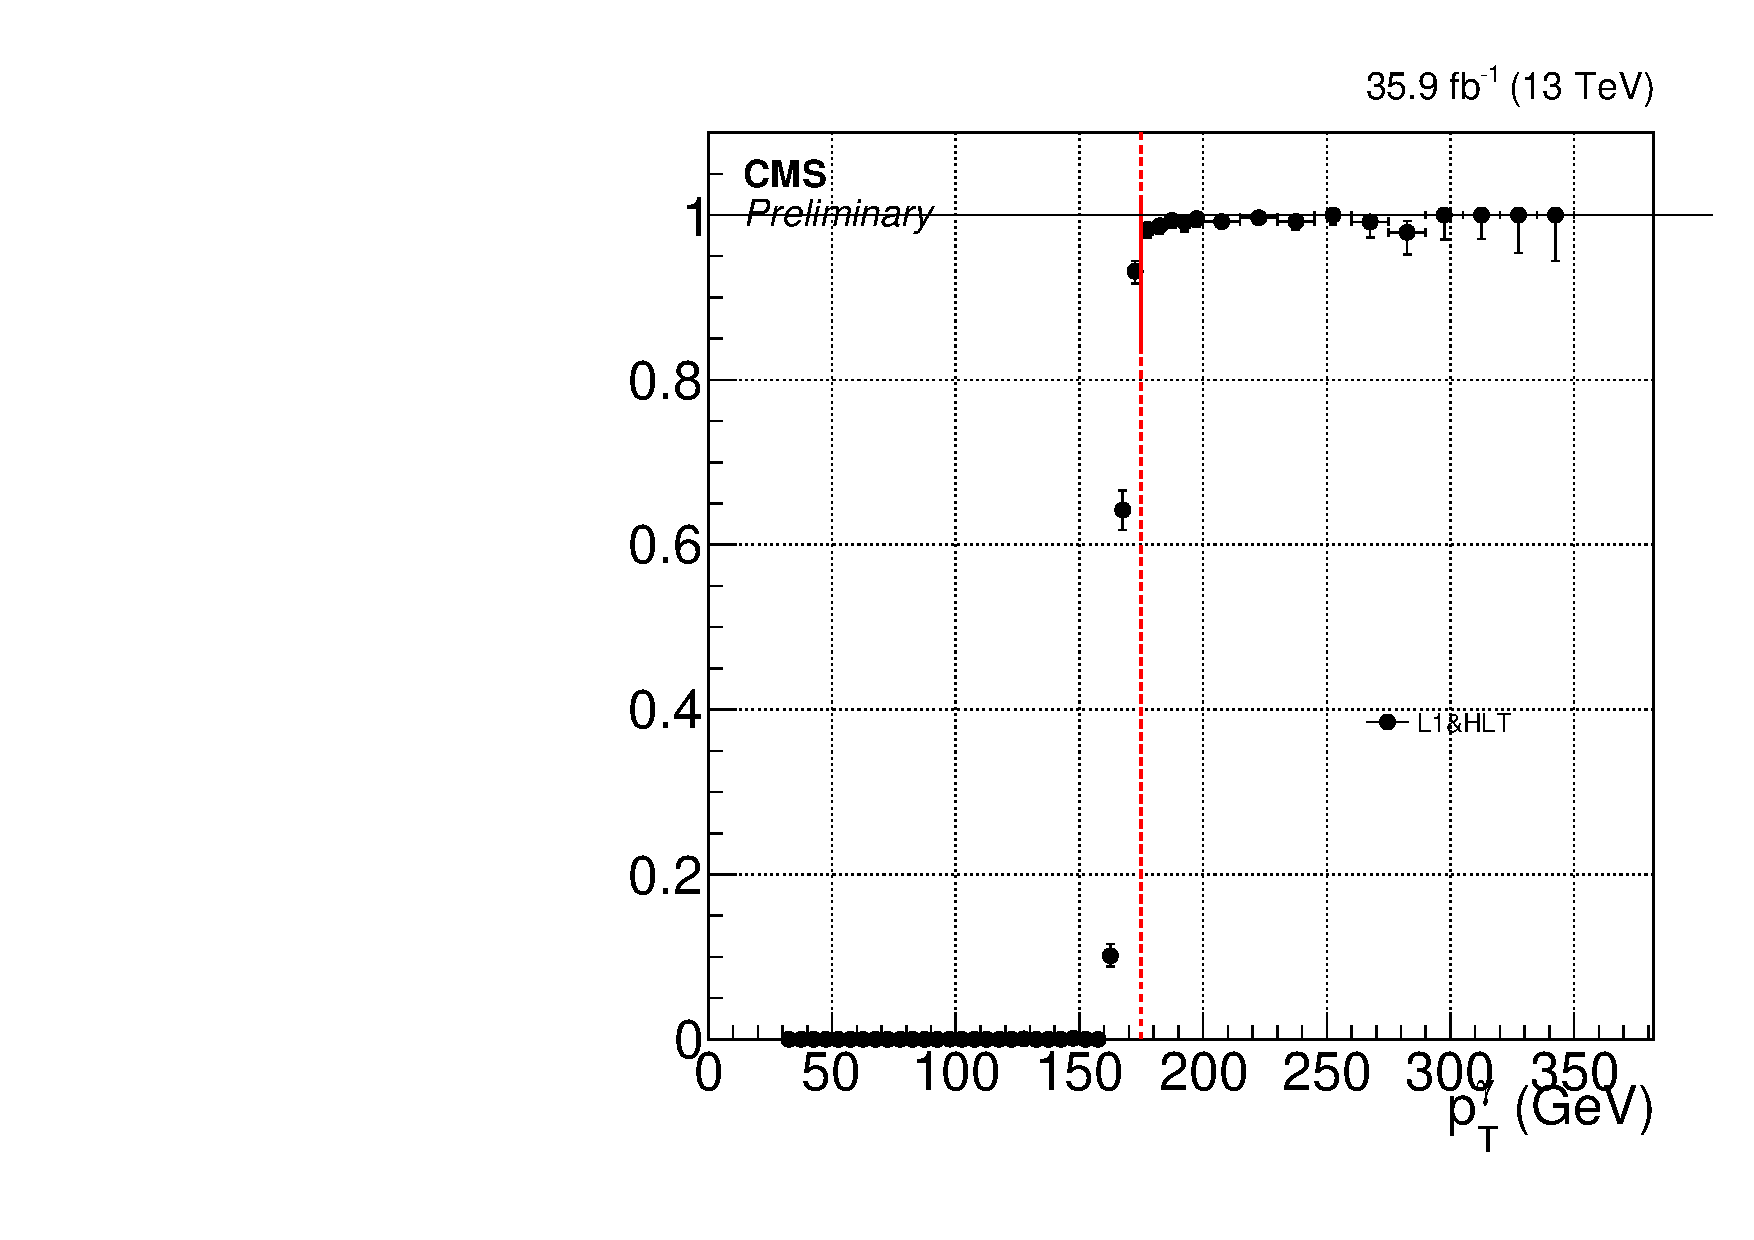
\includegraphics[width=0.48\linewidth]{Calibration/Figures/photon_elmu_sph165abs_ptzoom.pdf}
  \caption{
    The efficiency turn-on of the \texttt{HLT\_Photon165\_HE10} trigger for photons passing the candidate selection, measured using \Pgm\ + \egamma\ events from the SingleMuon data set. 
    Red vertical line corresponds to $\ET = 175\GeV.$
  }
  \label{fig:hlt_eff}
\end{figure}

For the first period of data taking, the \texttt{HLT\_Photon165\_HE10} trigger was seeded only by an isolated \egamma\ L1 trigger. 
This L1 seed becomes inefficient at high \ET\ due to a misconfiguration in the $H/E$ computation algorithm as indicated by the drop in efficiency at high-\ET\ shown in the left side of Figure~\ref{fig:l1_eff}. 
To mitigate the effect, in the later periods, the trigger was seeded by the logical \textbf{OR} of \texttt{SingleEG40} and \texttt{SingleJet} L1 triggers, combining multiple with various \pt\ thresholds.

Even with this addition, the measured trigger efficiency is not 100\% at the plateau, but it is flat with respect to \ET\ as shown on the right of Figure~\ref{fig:l1_eff}. 
In principle, the efficiency should be applied to all simulation-based background estimates whose normalization is fixed by theoretical calculation of the cross section.
However, the only simulation-based background processes with absolute normalization are those that contribute at $\mathcal{O}(1)$\%, with large systematic uncertainties. 
Therefore we deem the slight discrepancy of the trigger efficiency from unity as irrelevant.

\begin{figure}[htbp]
  \centering
  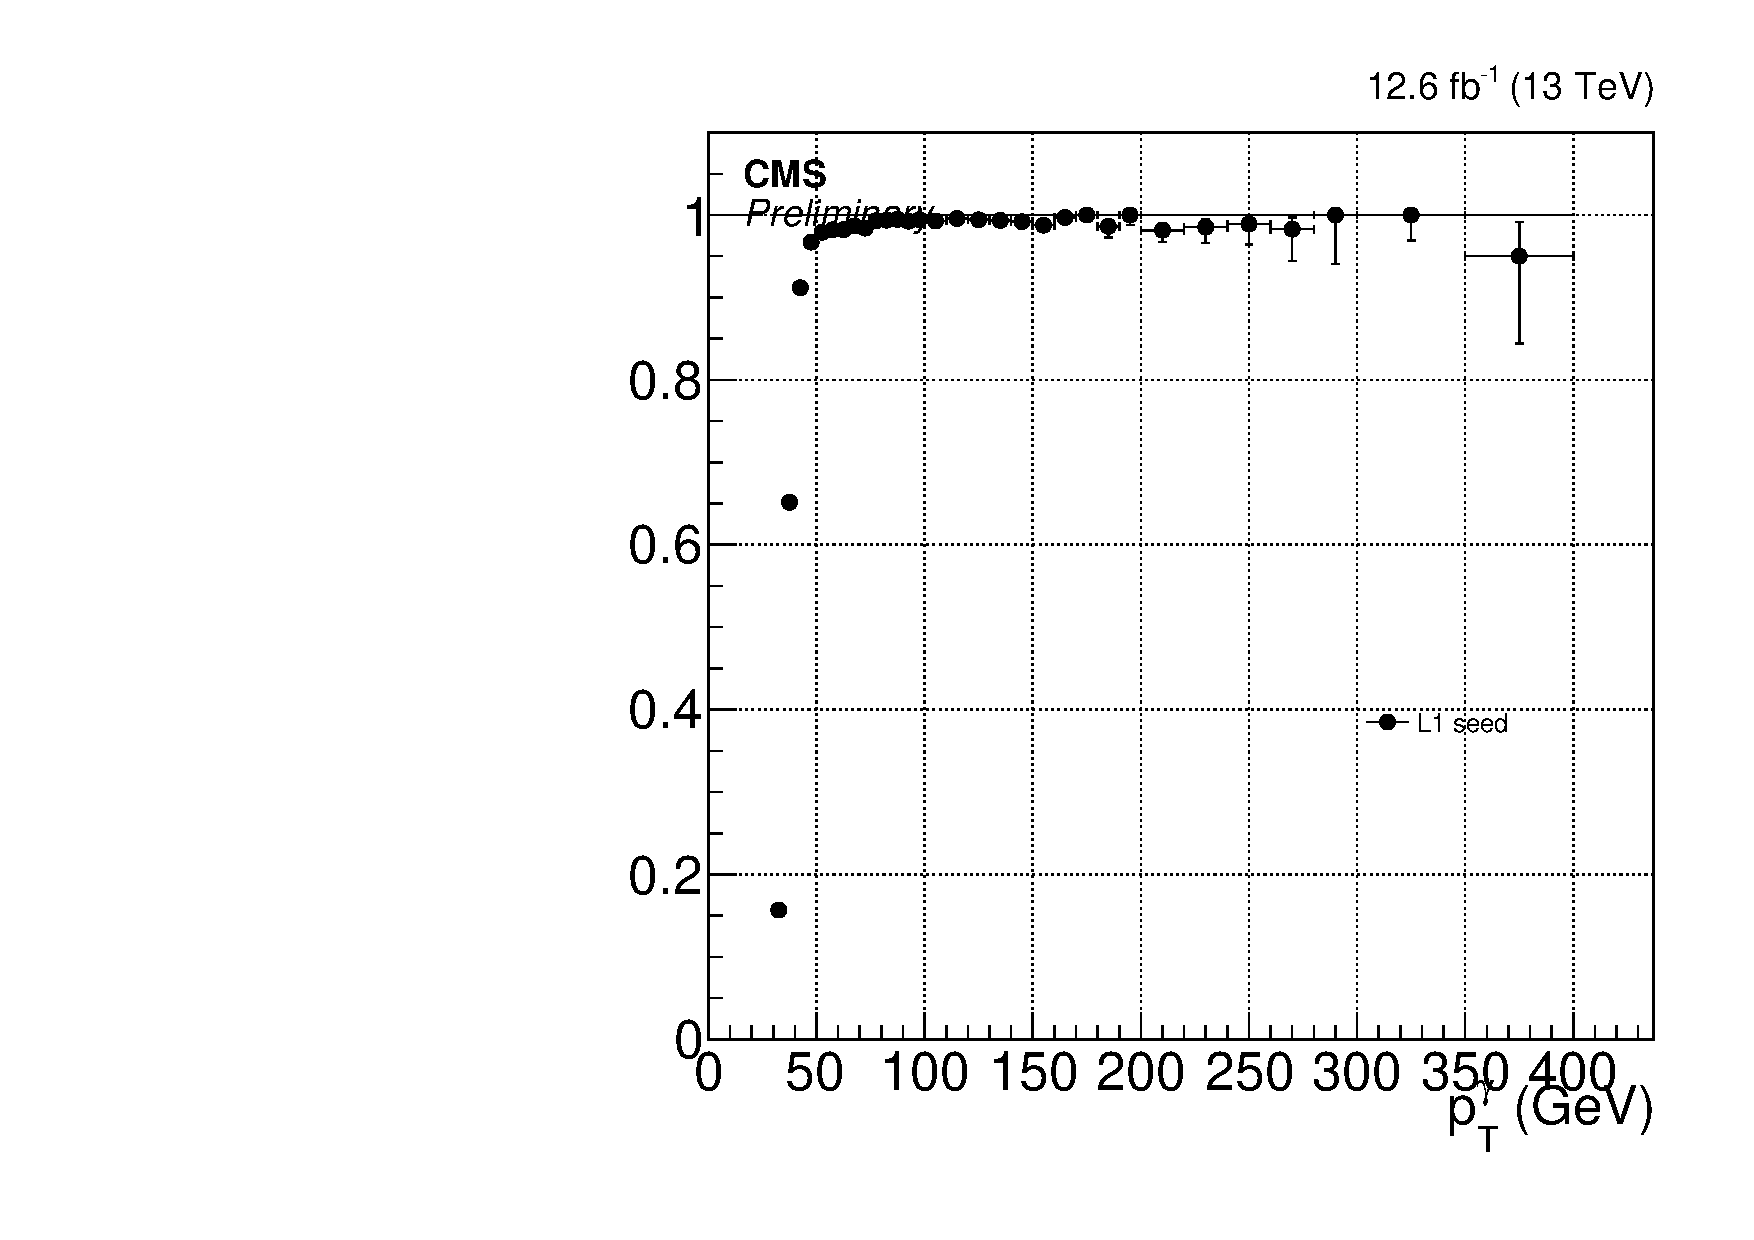
\includegraphics[width=0.48\linewidth]{Calibration/Figures/photon_elmuBCD_l1eg40_ptwide.pdf}
  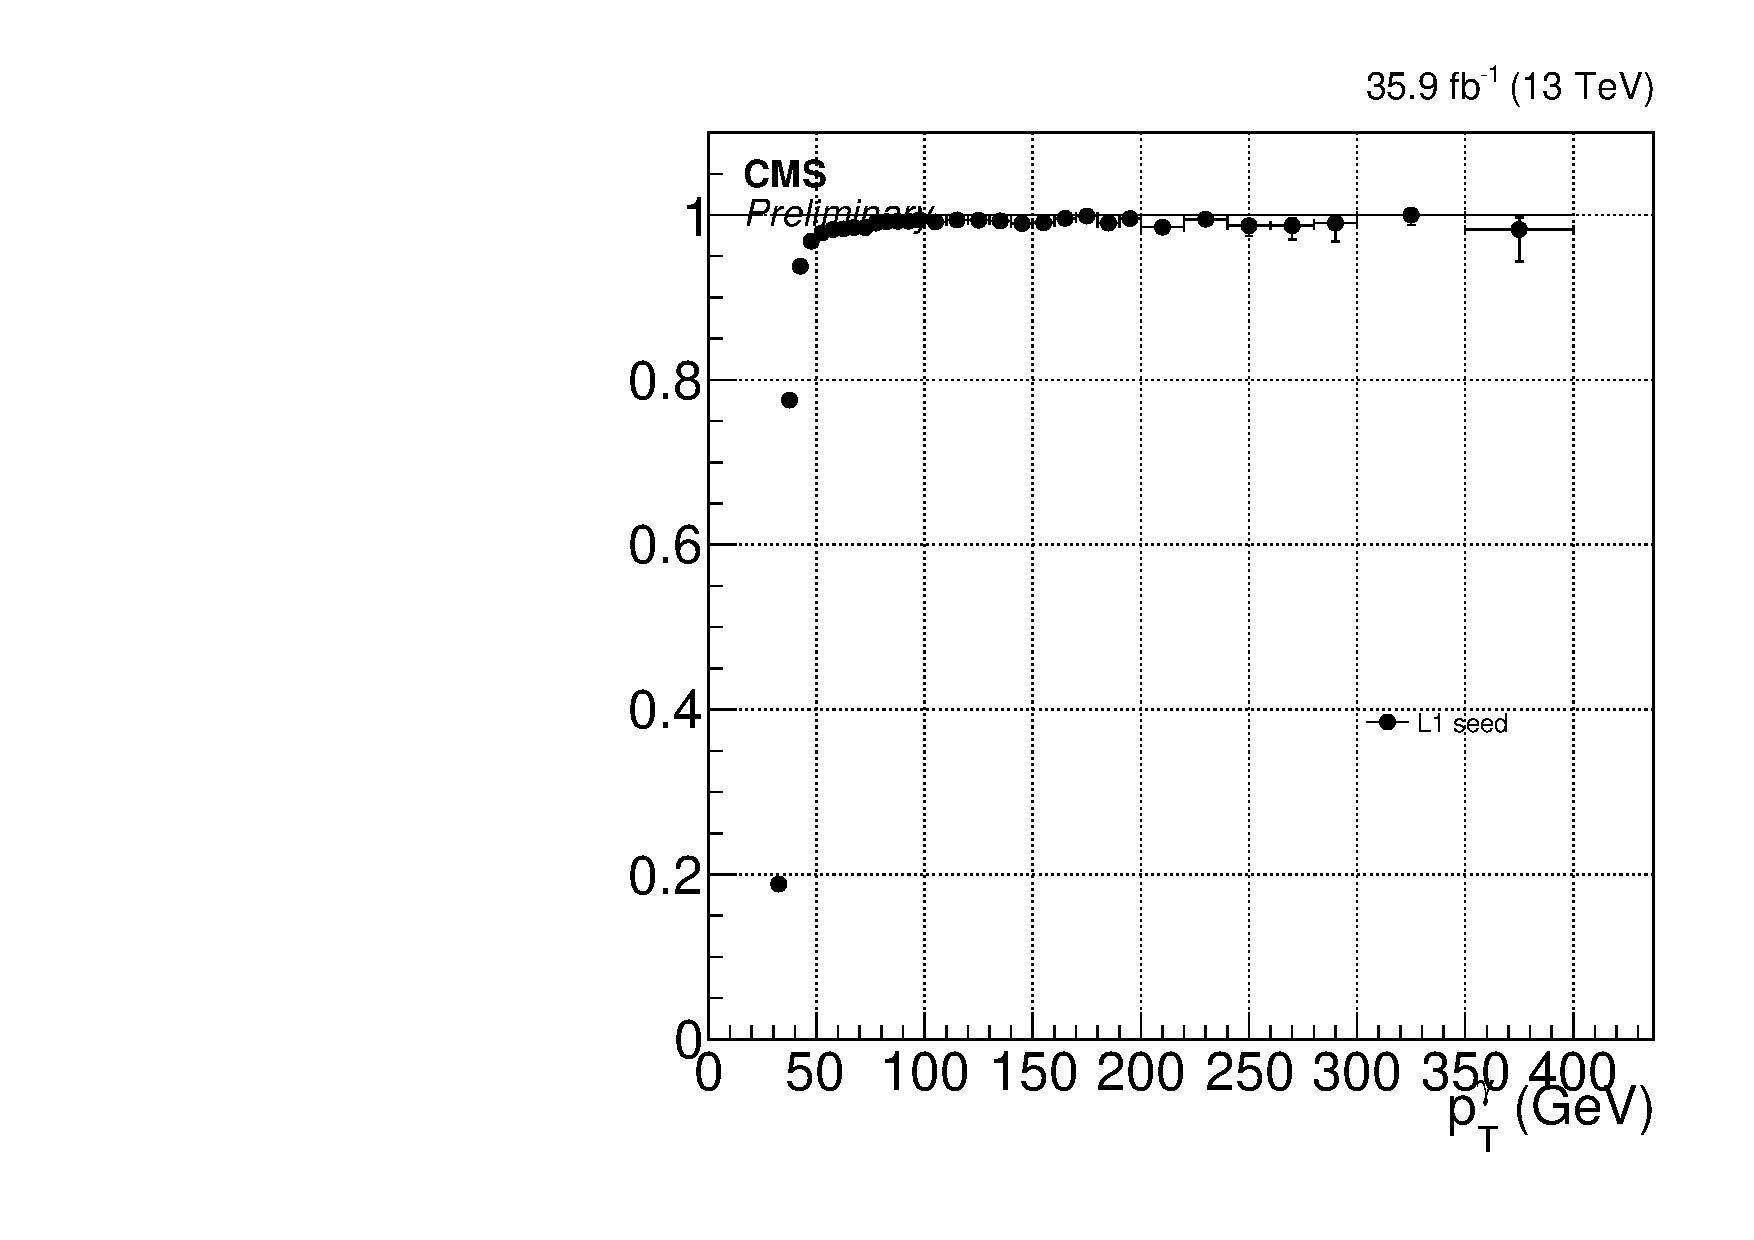
\includegraphics[width=0.48\linewidth]{Calibration/Figures/photon_elmu_l1all_ptwide.pdf}
  \caption{
    The efficiency of the L1 seed for the signal trigger in periods B and C (left) and the full data set (right). The drop in efficiency at high-\ET\ in the earlier period is fixed by the addition of \texttt{SingleJet} L1 seeds during the remainder of data-taking. 
  }
  \label{fig:l1_eff}
\end{figure}

\section{Event Selection}
\label{sec:event_selection}

%%% need to make a second pass to change language from paper version

From the recorded data, events are selected by requiring $\met > 170\GeV$ and at least one photon with $\ETg > 175\GeV$ in the fiducial region of the ECAL barrel ($\abs{\eta} < 1.44$) passing the selected presented in Section~\ref{sec:pf_photons}. 

Events with a high-\pt\ photon and large \met\ are subjected to further requirements to suppress SM background processes that feature a genuine high-energy photon, but not a significant amount of \met.
One such SM process is \gj, where an apparent large \met\ is often the result of a mismeasured jet energy.
In contrast to signal processes, \met is typically smaller than \ETg\ in these events, so requiring the ratio of \ETg\ to \met to be less than 1.4 rejects this background effectively with little effect on signal efficiency. 
Events are also rejected if the minimum opening angle between \ptvecmiss\ and the directions of the four highest \pt\ jets, \mindphijmet, is less than 0.5. 
Only jets with $\pt > 30\GeV$ and $\abs{\eta} < 5$ are considered in the \mindphijmet\ calculation. 
In the \gj\ process, rare pathological mismeasurement of \ETg\ can also lead to large \met. 
For this reason, the candidate photon \ptvec\ and \ptvecmiss\ must be separated by more than 0.5 radians. 
Another SM process to be rejected is \wlng, for which events are vetoed if they contain an electron or a muon with $\pt > 10\GeV$ that is separated from the photon by $\dR > 0.5$.
Furthermore, using features described in Section~\ref{sec:halo_estimate}, the signal region is split into two parts according to $\phi$ to constrain the beam halo normalization. 
The region defined by $\abs{\sin(\phi)} < \sin(0.5)$ is called the horizontal region, and its complement in $\phi$ is called the vertical region.

The residual contributions from the \wlng\ process, where the lepton could not be identified or was out of the detector acceptance, are modeled by fitting to observed data, as described in Section~\ref{sec:irreducible}. 
The same method is employed to model the contribution from the \zinvg\ process to the signal region. 
This method utilizes control regions where one or two leptons (electrons or muons) are identified in addition to the photon, as defined in the following.

The single-electron (single-muon) control region is defined by a requirement of exactly one electron (muon) with $\pt > 30\GeV$ and $\abs{\eta} < 2.5\,(2.4)$ in addition to a photon requirement that is identical to the one for the signal region. 
To suppress the contributions from large-\met\ processes other than \wlng, the transverse mass $\mt = \sqrt{\smash[b]{2\met\pt^{\ell}[1-\cos\Delta\phi(\ptvecmiss,\ptvec^{\ell})]}}$ must be less than $160\GeV$.
Additionally, for the single-electron control region, \met\ must be greater than 50\GeV\ to limit the contribution from the \gj\ process, where a jet is misidentified as an electron. 
Finally, the recoil vector $\vec{U} = \ptvecmiss + \ptvec^{\ell}$, which serves as this region's analogue for \ptvecmiss\ in the signal region, must satisfy identical requirements to those for the \ptvecmiss\ in the signal region.

The dielectron (dimuon) control region is defined by exactly two electrons (muons) in addition to the photon, with $60 < m_{\ell\ell} < 120\GeV$, where $m_{\ell\ell}$ is the invariant mass of the dilepton system. 
The recoil vector of this region is $\vec{U} = \ptvecmiss + \sum\ptvec^{\ell}$ and must satisfy identical requirements to those for the \ptvecmiss\ in the signal region.

\section{Irreducible backgrounds}
\label{sec:irreducible}

\subsection{Simulation of \vg\ Processes}
\label{sec:vgmc}

The \zinvg\ and \wlng\ background contributions are modeled using MC simulations.
Samples generated at the leading order (LO) in QCD by \MADGRAPH5 with up to two additional partons and a generator-level requirement of $\ETg > 130\GeV$ are employed for this purpose.

A study using a privately generated aMC@NLO sample with high \ETg\ threshold confirms that the predicted kinematic distributions would not change drastically by using the NLO sample. 
Figures~\ref{fig:zg_nlo_lo} and \ref{fig:wg_nlo_lo} show the comparisons of the private aMC@NLO samples and the \MADGRAPH5 samples used for the background estimation in the key kinematic distributions.

\begin{figure}[htbp]
  \centering
  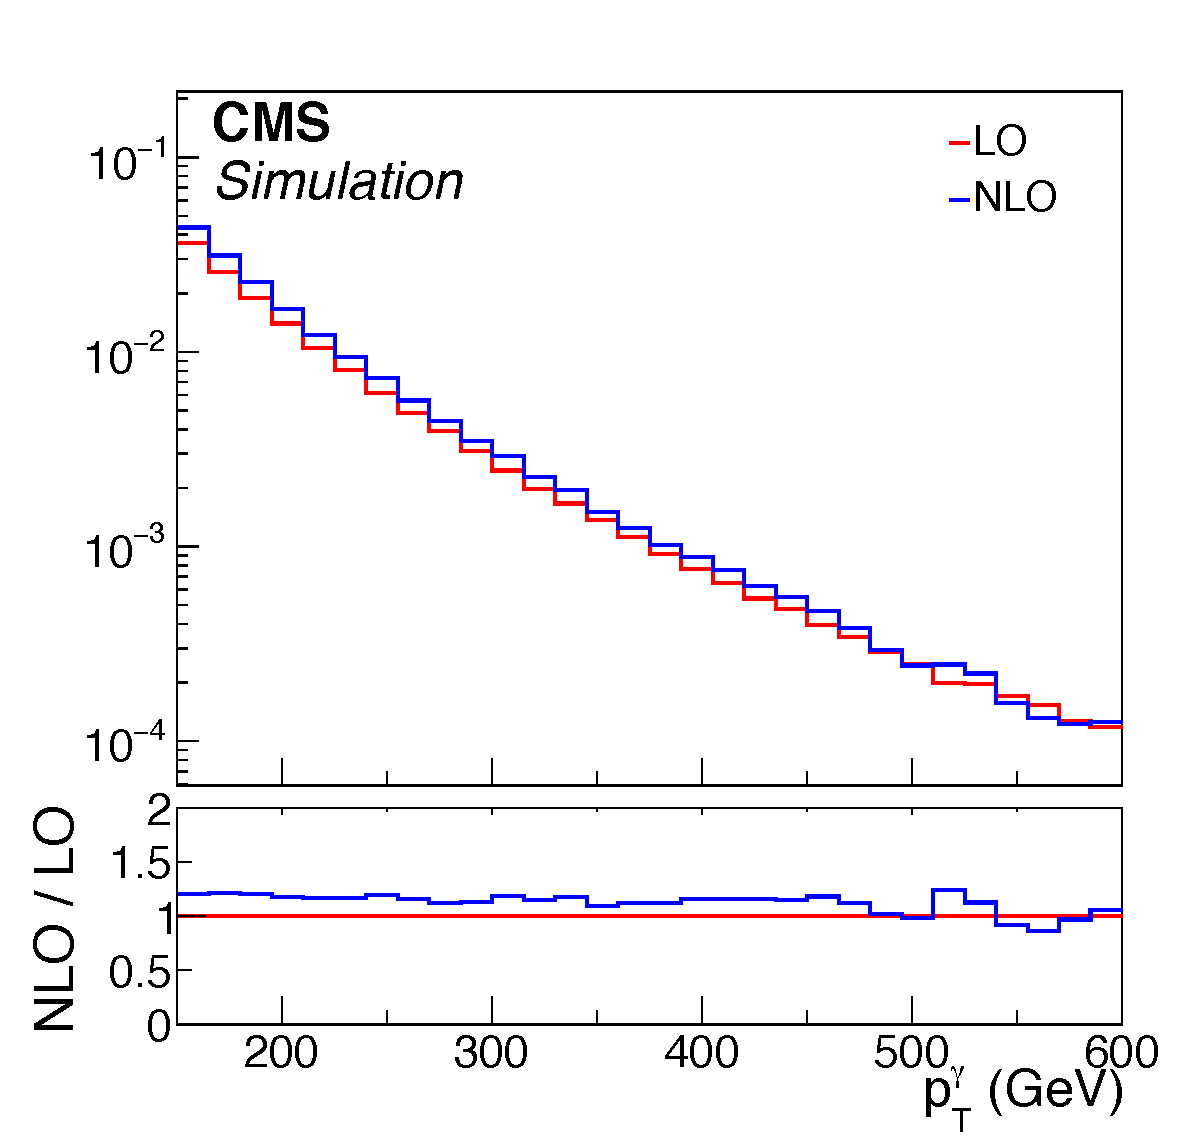
\includegraphics[width=0.32\textwidth]{Analysis/Figures/kfactor/ZG_ptg.pdf}
  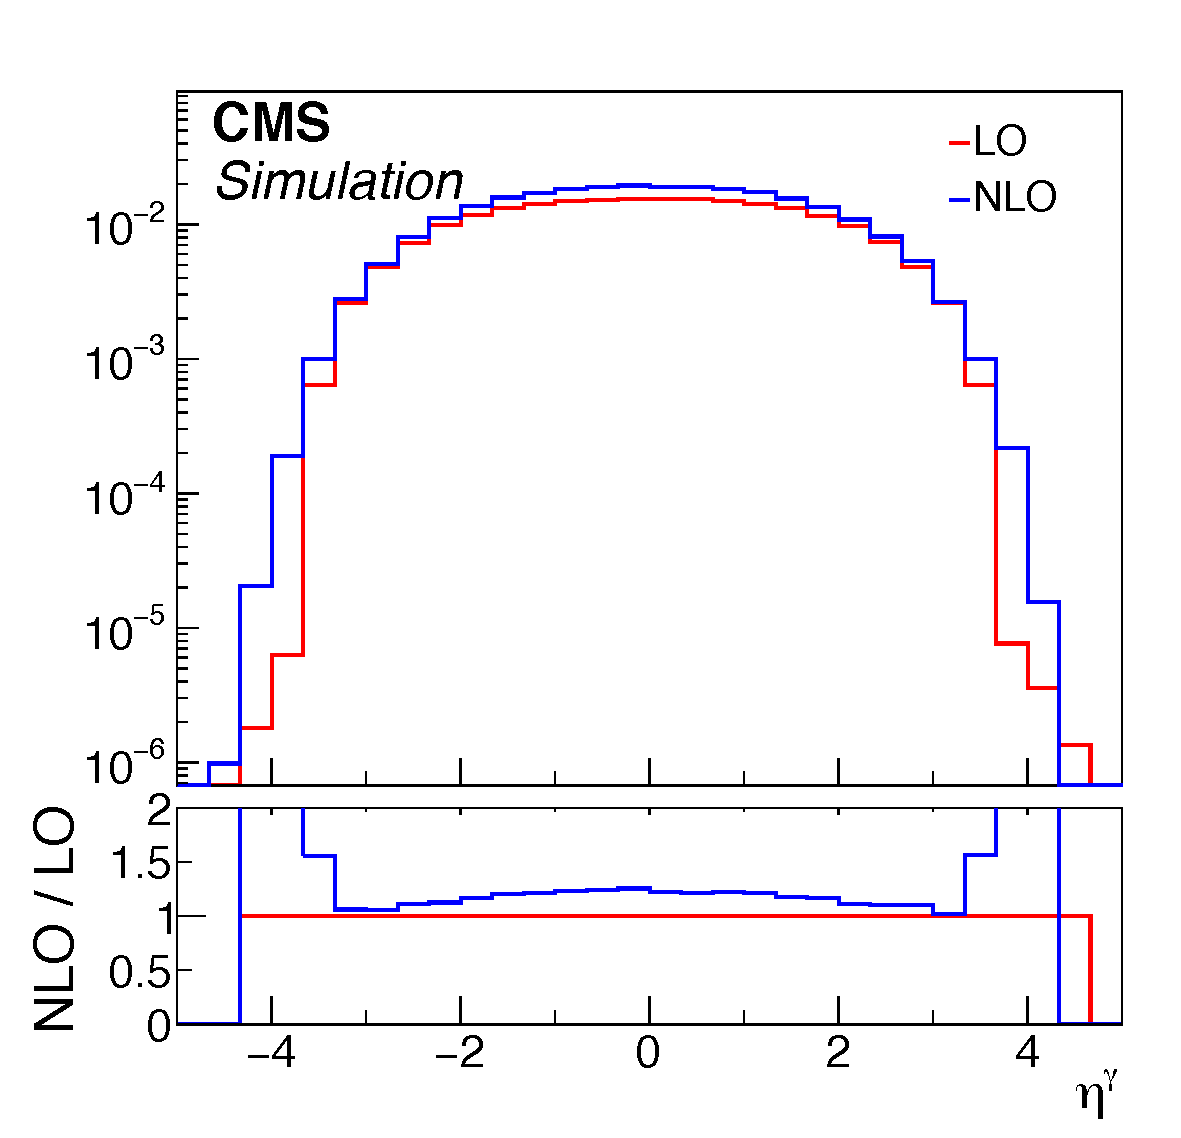
\includegraphics[width=0.32\textwidth]{Analysis/Figures/kfactor/ZG_etag.pdf}
  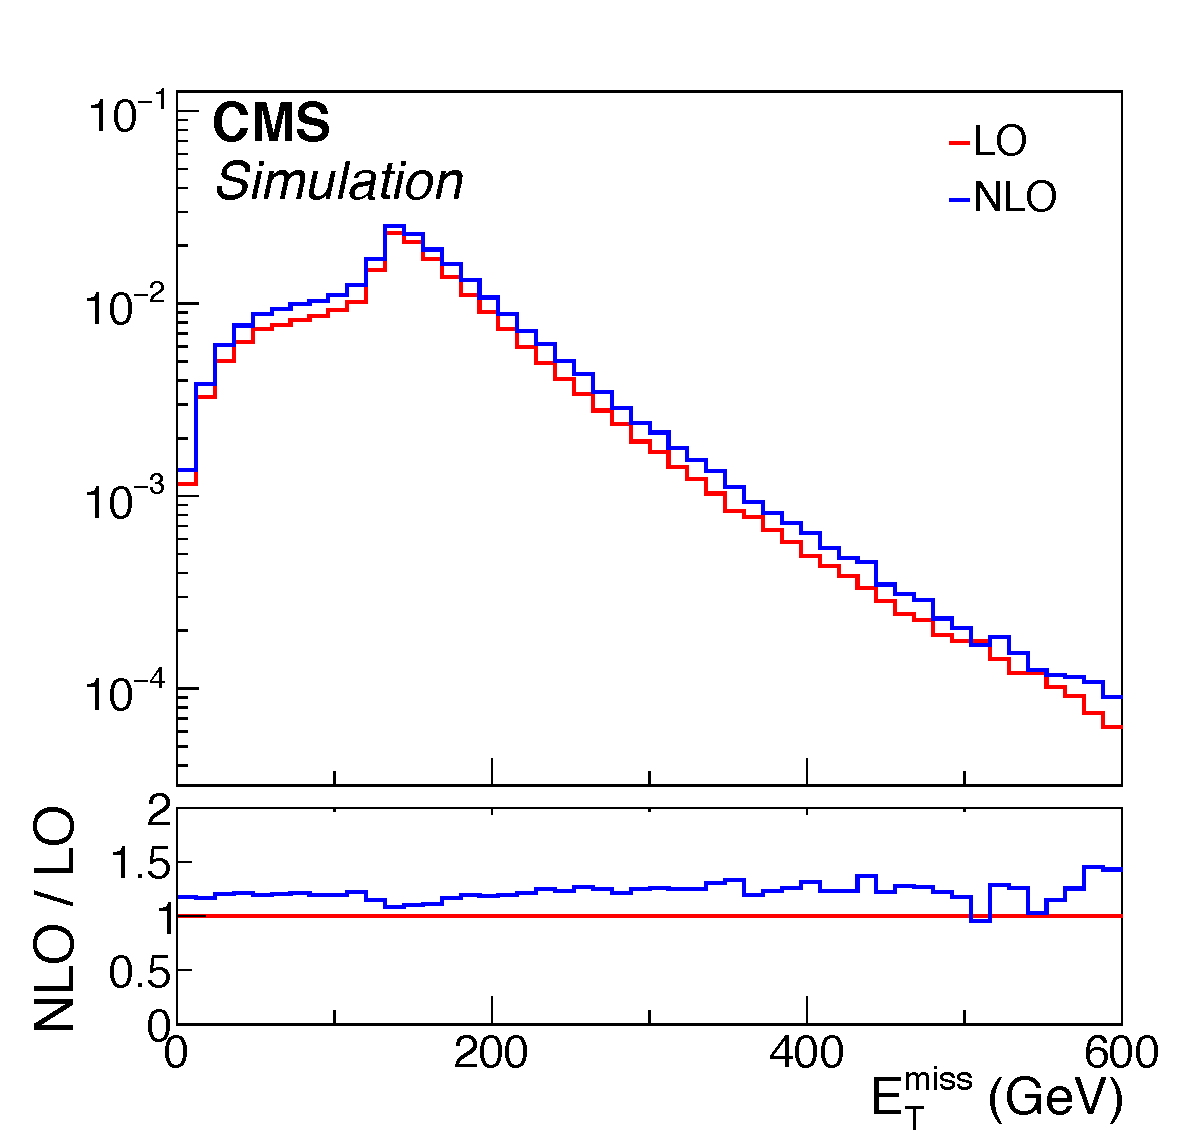
\includegraphics[width=0.32\textwidth]{Analysis/Figures/kfactor/ZG_met.pdf}
  \caption{
    Distributions of \ETg\ (left), $\eta^{\Pgg}$ (middle), and $\pt^{\PZ}$ (right) in \zinvg\ process from the private aMC@NLO sample (blue) and the LO sample used for background prediction (red) along with the NLO / LO ratios.
  }
  \label{fig:zg_nlo_lo}
\end{figure}
\begin{figure}[htbp]
  \centering
  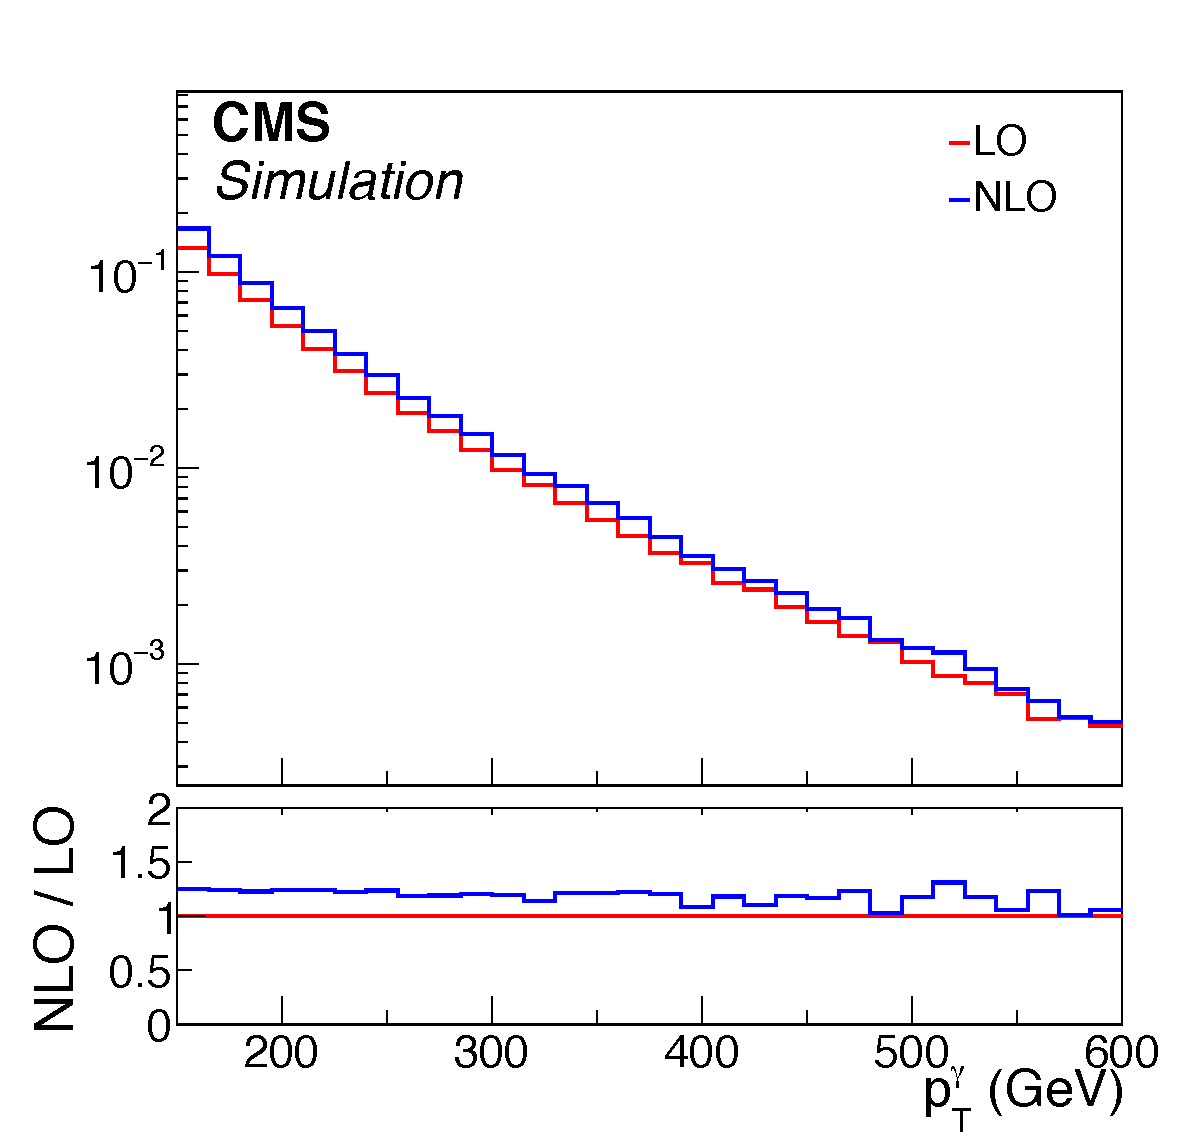
\includegraphics[width=0.32\textwidth]{Analysis/Figures/kfactor/WG_ptg.pdf}
  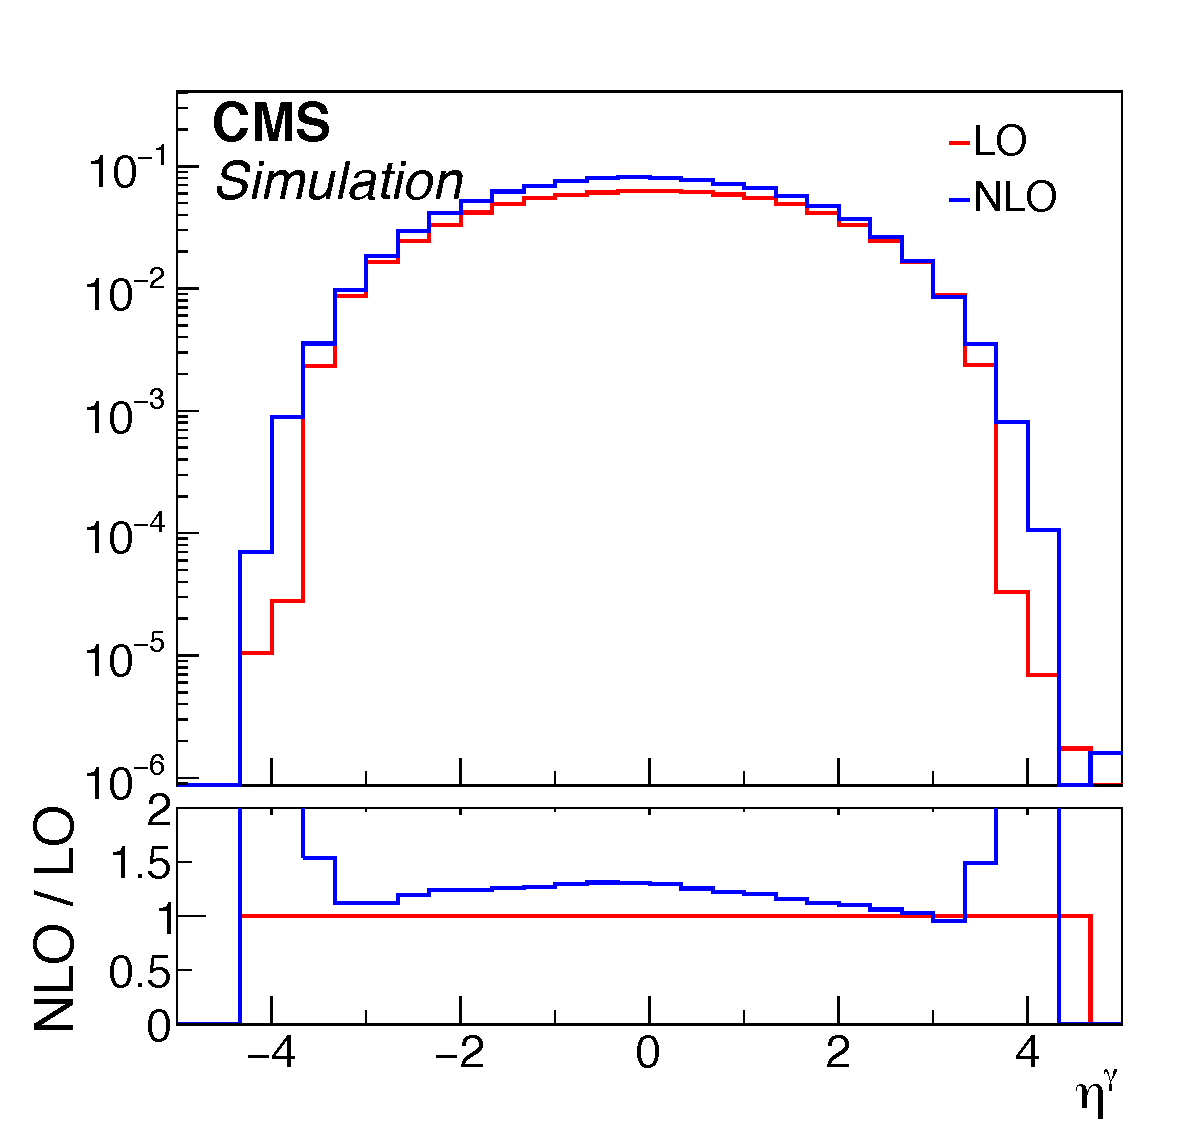
\includegraphics[width=0.32\textwidth]{Analysis/Figures/kfactor/WG_etag.pdf}
  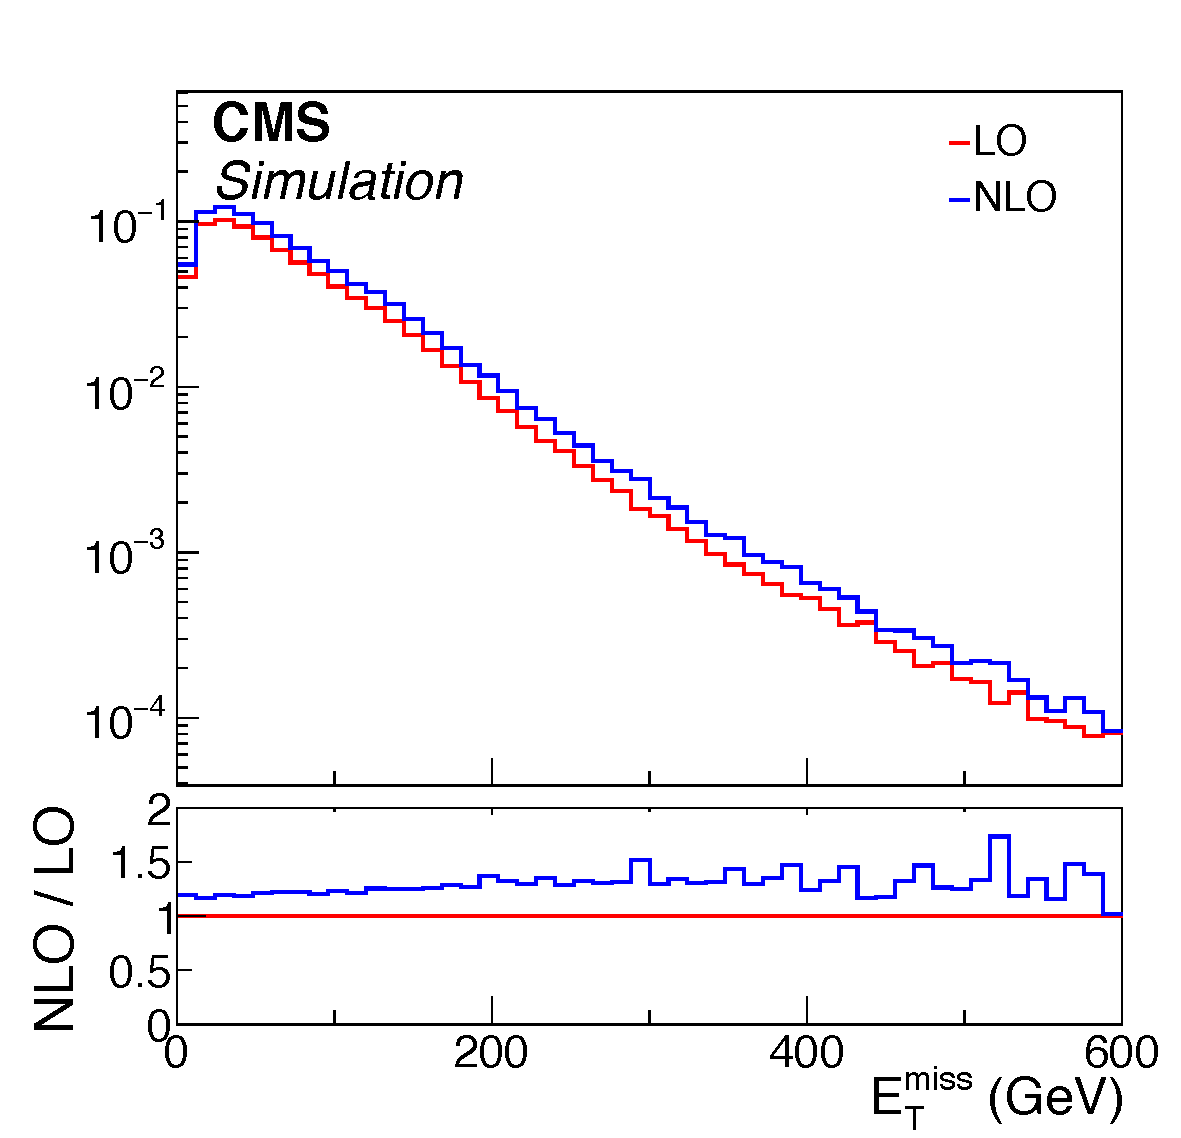
\includegraphics[width=0.32\textwidth]{Analysis/Figures/kfactor/WG_met.pdf}
  \caption{
    Distributions of \ETg\ (top left), $\eta^{\Pgg}$ (top right), and $\pt^{\PW}$ (bottom left) in \wlng\ process from the private aMC@NLO sample (blue) and the LO sample used for background prediction (red) along with the NLO / LO ratios.
  }
  \label{fig:wg_nlo_lo}
\end{figure}

To approximate the QCD higher-order effects, \zinvg\ and \wlng\ events are reweighted with \ETg\ by the factors given in Tab.~\ref{tab:zg_kfactors}. 
These factors are the ratios of QCD next-to-next-to leading order (NNLO) differential cross sections calculated by Grazzini et al.~\cite{Bozzi:2010xn} to the LO cross sections given in the centrally produced samples. 
(Note that the denominator cross section includes contributions from processes with up to two additional partons, and is therefore not a LO cross section in the strict sense of the word. V\Pgg\ k-factors found in literature can be $\gg 1$ at high \ETg, if the denominator only accounts for the cross section of $\Pq\Paq\rightarrow\mathrm{V}\Pgg$ process.)

\begin{table}
  \begin{center}
    \begin{tabular}{ l | r | r }
      \ETg range (GeV) & \zinvg & \wlng \\
      \hline
      $[175, 190]$ & 1.44 & 1.40 \\
      $[190, 250]$ & 1.41 & 1.37 \\
      $[250, 400]$ & 1.35 & 1.31 \\
      $[400, 700]$ & 1.29 & 1.26 \\
      $[700, \infty)$ & 1.15 & 1.15 \\
    \end{tabular}
    \caption{NNLO / LO correction factors for \zinvg\ and \wlng\ samples.}
    \label{tab:zg_kfactors}
  \end{center}
\end{table}

Additionally, higher-order electroweak correction factors are also applied as a function of \ETg. 
Out of various electroweak higher-order effects, ones that can give sizeable
($\gg\mathcal{O}(\alpha)$) corrections to the cross section are Sudakov suppression at high boson \pt\ and potentially the addition of photon-induced scattering processes~\cite{Denner:2014bna,Denner:2015fca}. 
We apply the correction factors shown in Figure~\ref{fig:ewk_correction}, which are combinations of Sudakov suppression factors and photon-induced enhancements, and are provided by the authors of Ref.~\cite{Denner:2015fca} in addition to the NNLO QCD correction.

\begin{figure}[htbp]
  \centering
  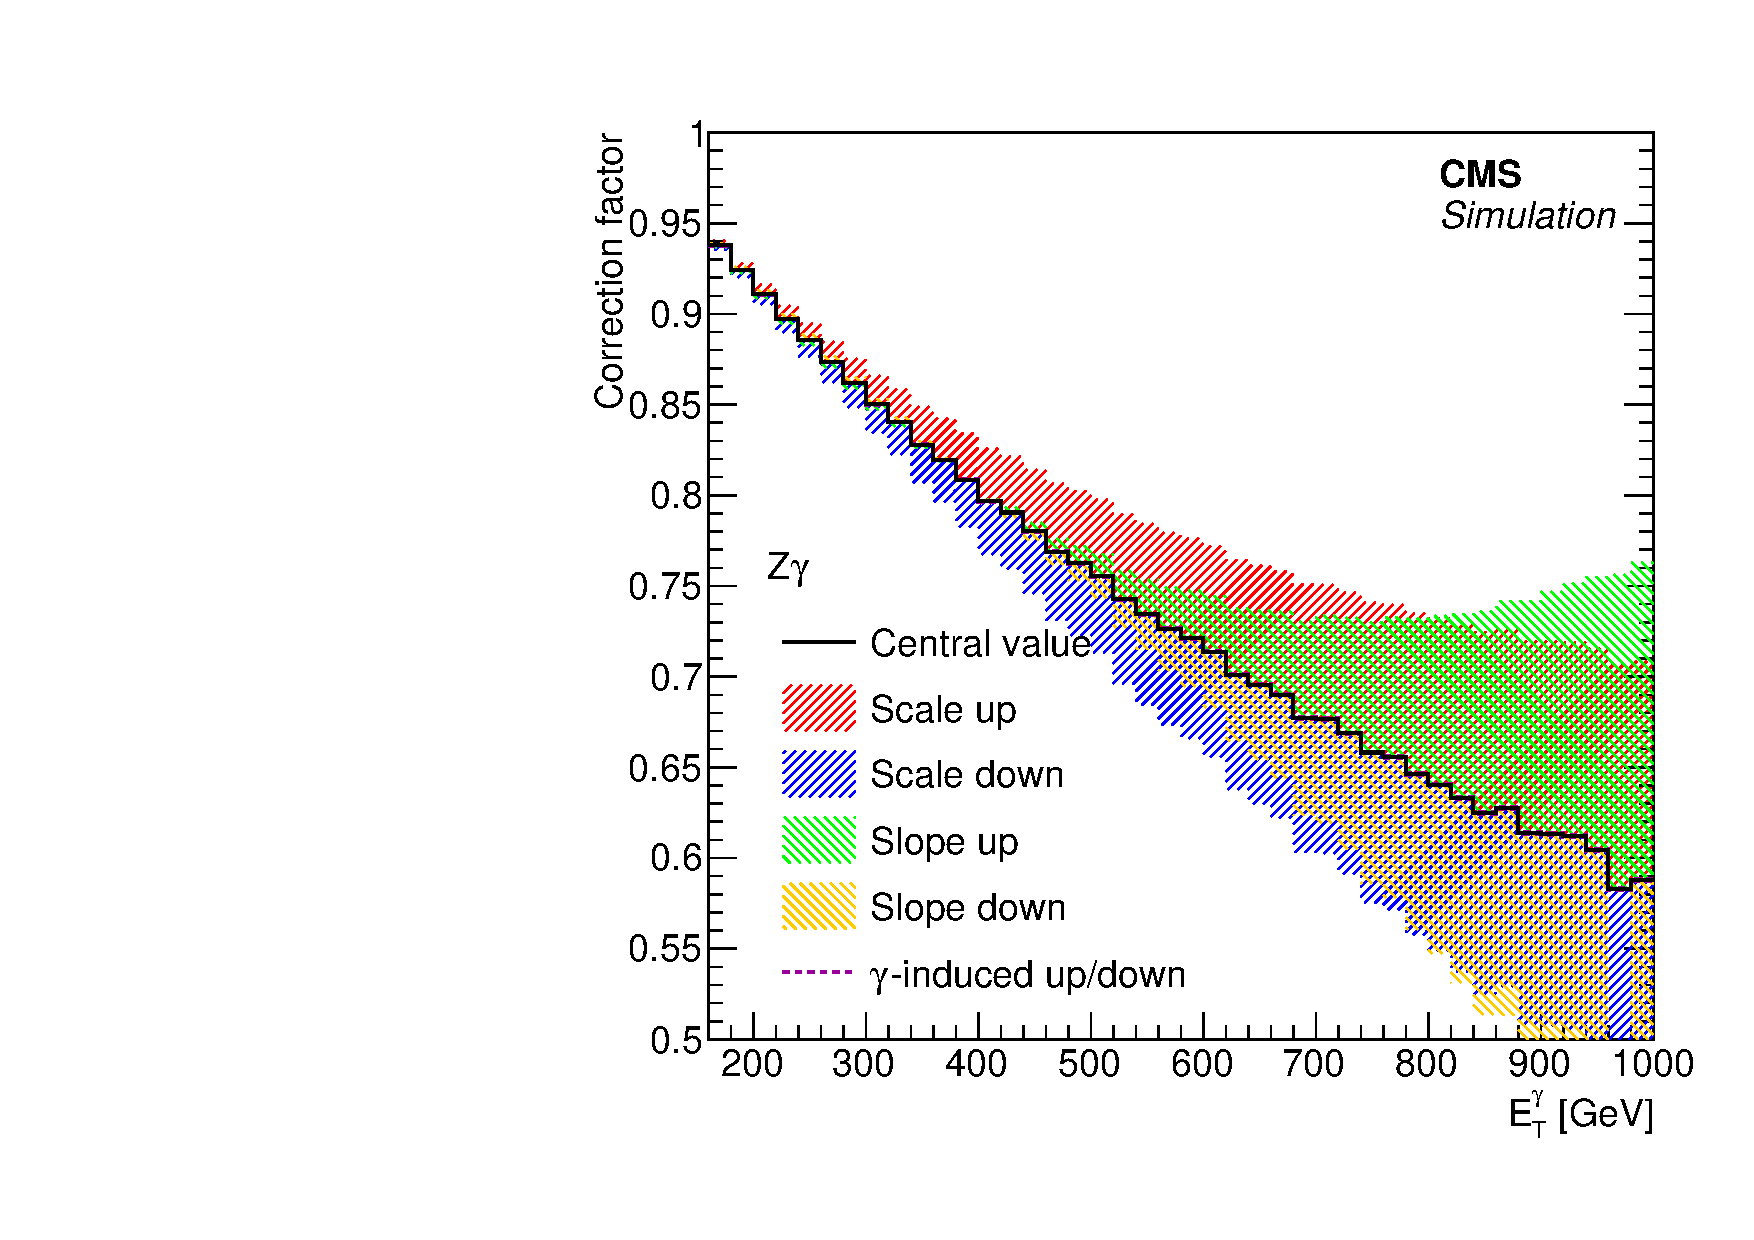
\includegraphics[width=0.32\textwidth]{Analysis/Figures/ewkcorr/zg.pdf}
  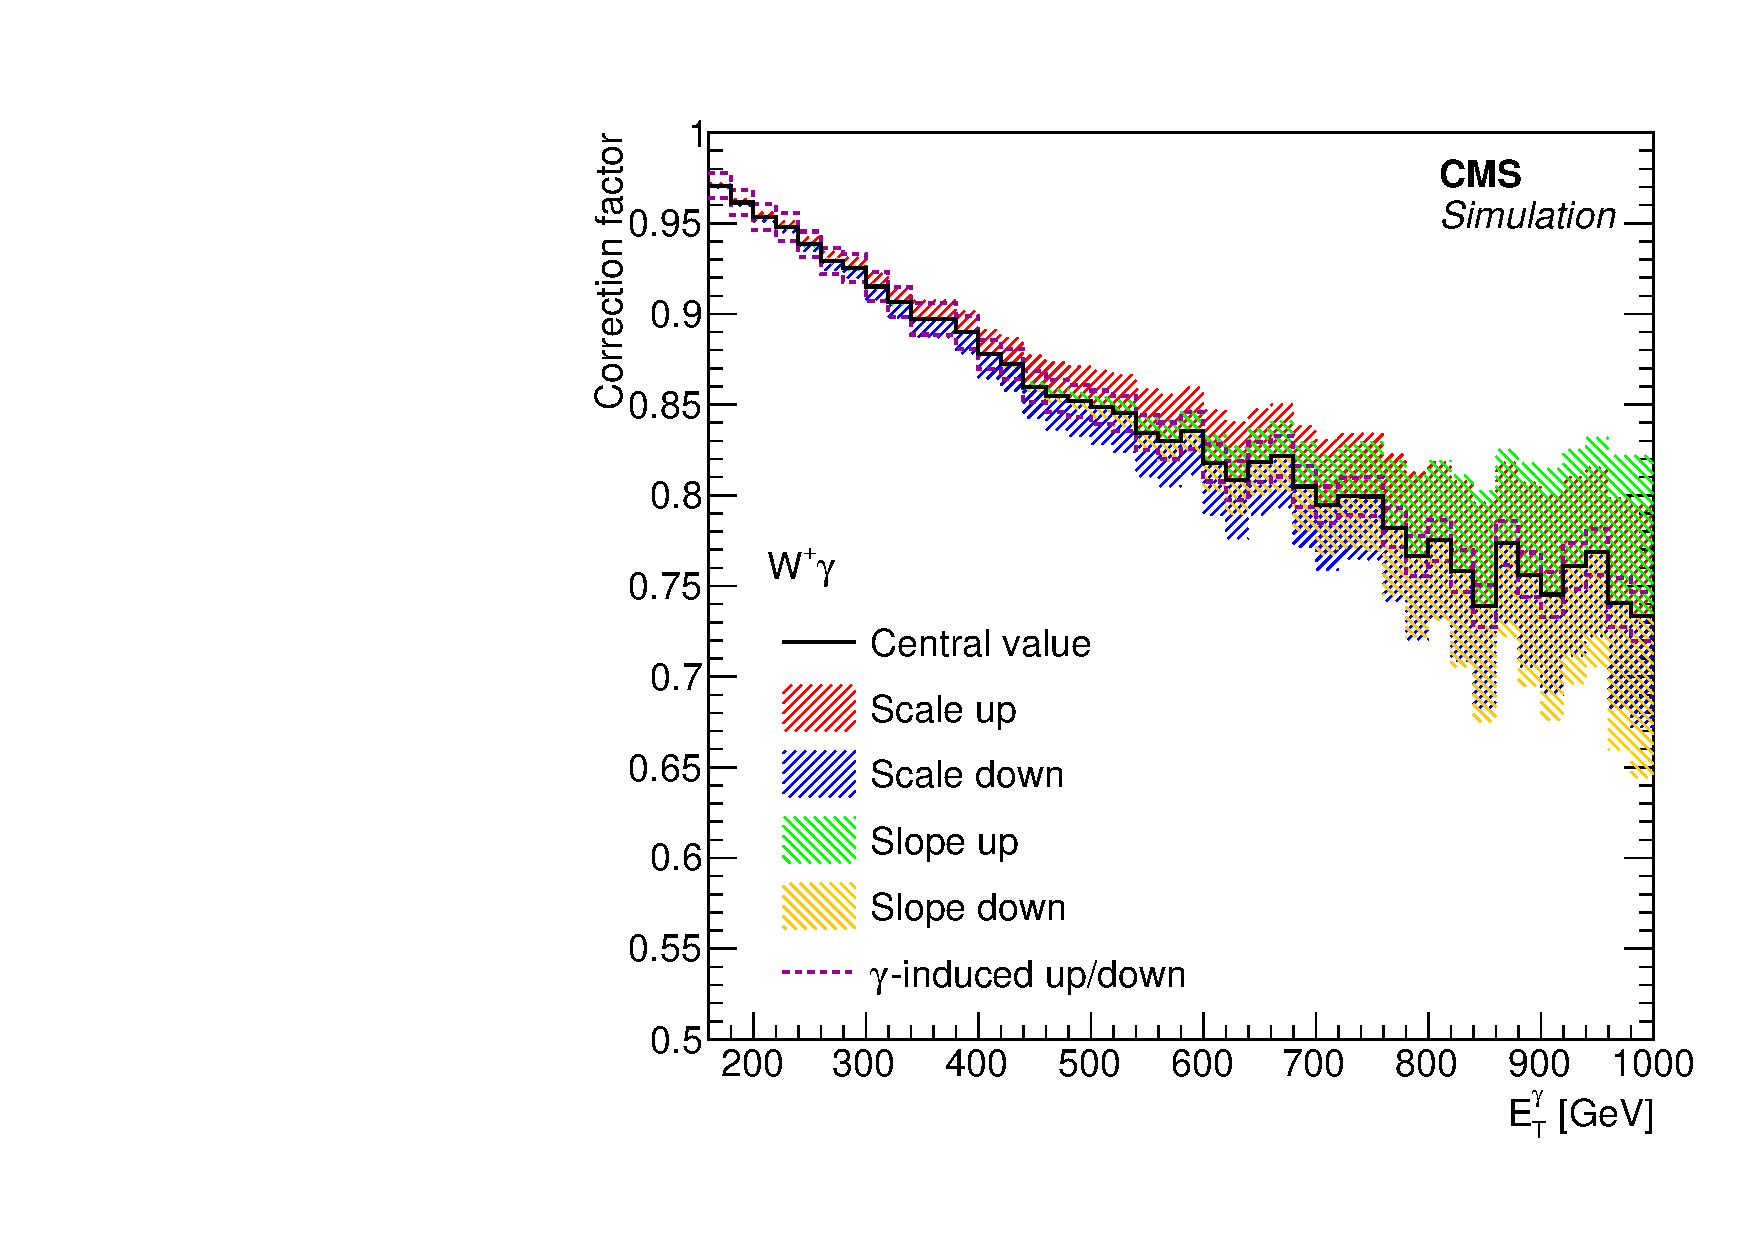
\includegraphics[width=0.32\textwidth]{Analysis/Figures/ewkcorr/wgplus.pdf}
  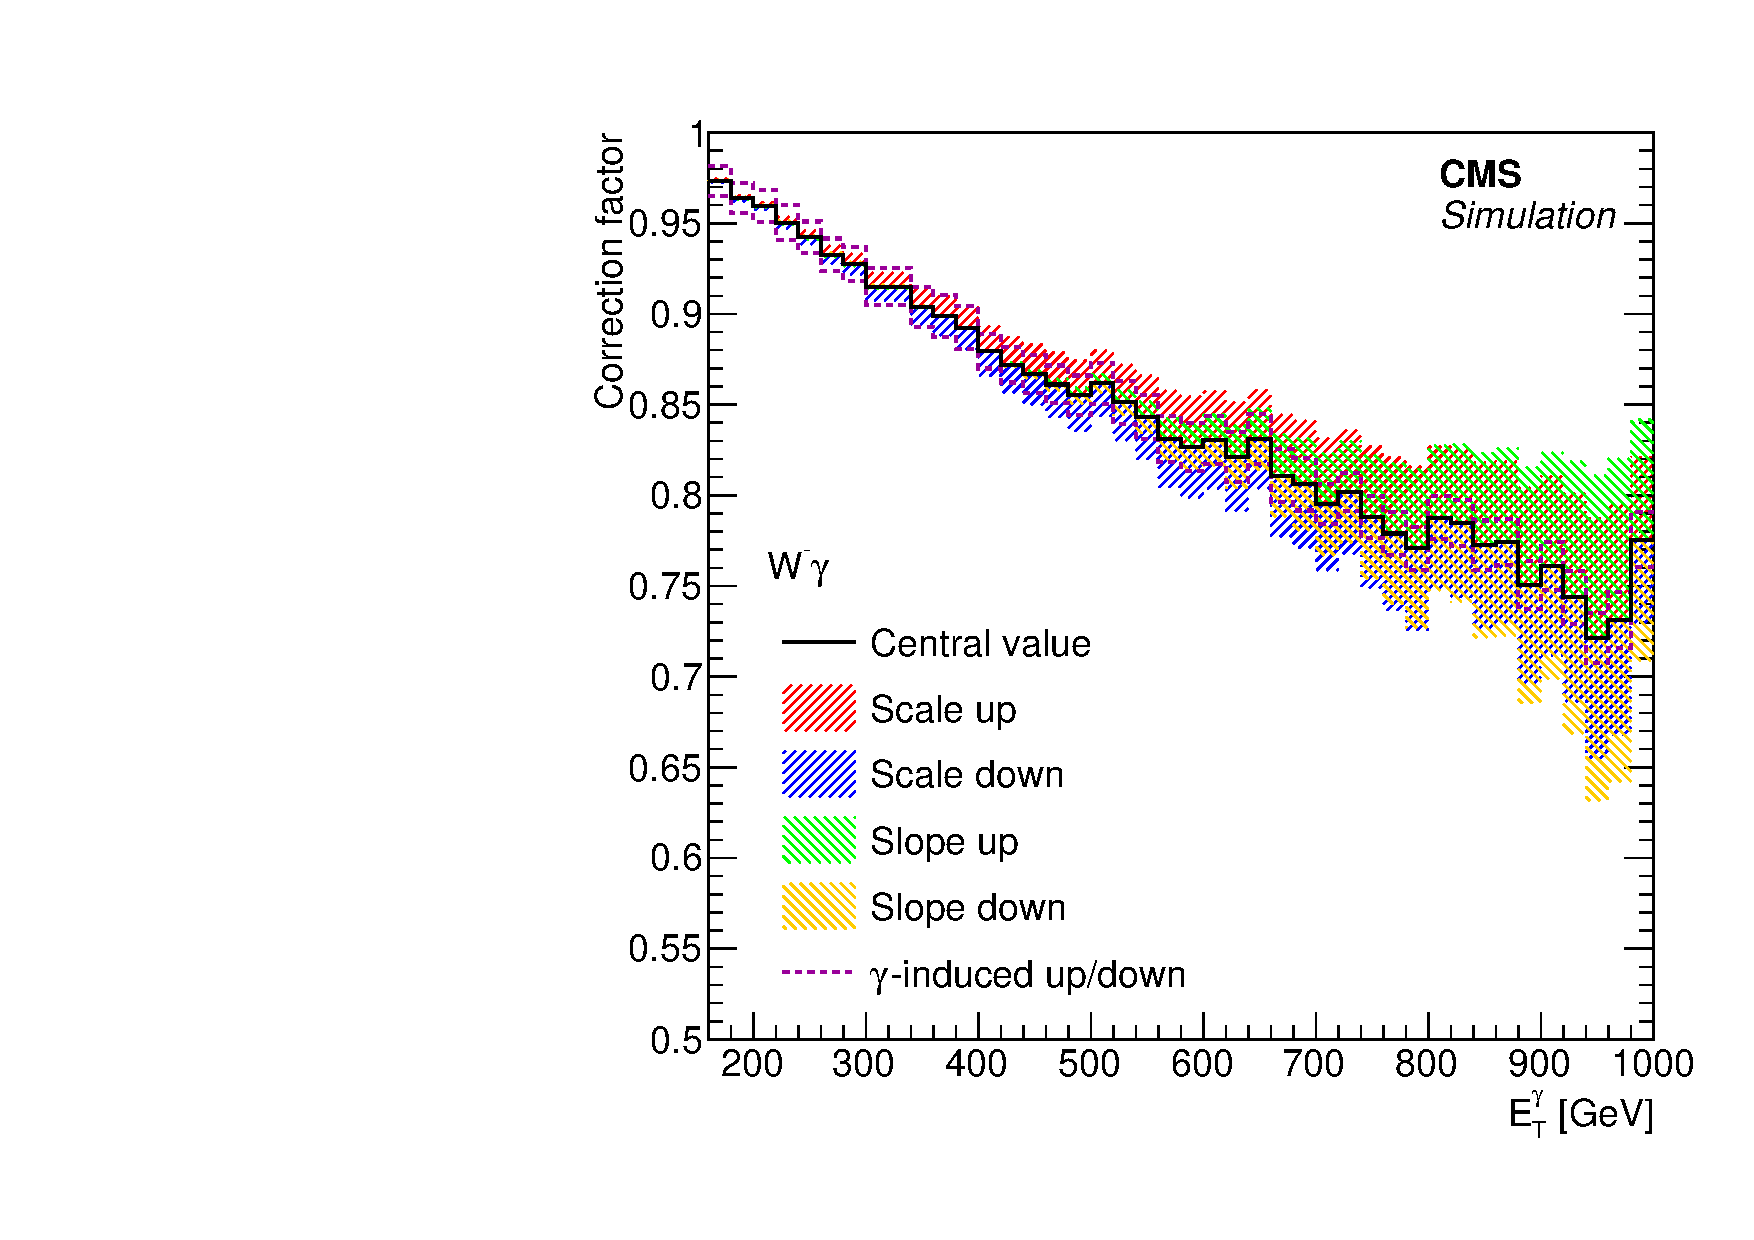
\includegraphics[width=0.32\textwidth]{Analysis/Figures/ewkcorr/wgminus.pdf}
  \caption{
    Electroweak NLO cross section corrections as a function of photon \pt\ for \zinvg\ (left), $\PW^{+}+\Pgg$ (middle), and $\PW^{-}+\Pgg$ (right) processes, overlaid with uncertainty bands. 
    See text for descriptions of the individual components of the uncertainty.
    The uncertainty due to \Pgg-induced production is negligible in \zinvg\ production.
  }
  \label{fig:ewk_correction}
\end{figure}

The differential cross section after the full higher-order corrections is therefore denoted as
\begin{equation}
  d\sigma^{\text{NNLO QCD}+\text{NLO EW}} = d\sigma^{\text{LO}} k^{\text{NNLO QCD}} (1 + \kappa^{\text{EW Sudakov}} + \kappa^{\text{EW} \Pq\Pgg}),
\end{equation}
where $k^{\text{NNLO QCD}} = d\sigma^{\text{NNLO QCD}} / d\sigma^{\text{LO}}$, and the two $\kappa$ terms are the Sudakov suppression and photon-induced enhancement components of the electroweak
correction, respectively.

Furthermore, subtle differences between simulation and observation in the reconstruction and identification efficiencies for various particle candidates are accounted for with the set of selection efficiency correction factors $\rho$. 
The value of an individual $\rho$ typically lies within a few percent of unity. 
Further details on the measurement and values of various $\rho$ are found in Chapter~\ref{chap:calibration}.

Four sources of systematic uncertainties considered for \ETg\ distribution ratios of the \vg\ processes are higher-order QCD corrections, higher-order EWK corrections, choice of PDF set, and data-to-simulation correction factors $\rho$. 
The four uncertainties are all considered as correlated between the \ETg\ bins.

The higher-order QCD renormalization and factorization scale uncertainties on the NNLO cross sections are assessed by varying the respective scales by factor 2 and 0.5 during the cross section computation. 
These uncertainties are between 7-8\%, varying bin by bin, and are considered uncorrelated in the ratio between the \zinvg\ and \wlng\ processes.

Theoretical uncertainties on the electroweak corrections are not well understood to date.  
We estimate the magnitude of the uncertainty on $\kappa^{\text{EW Sudakov}}$ and $\kappa^{\text{EW} \Pq\Pgg}$ to be $(\kappa^{\text{EW Sudakov}})^2$ and $\kappa^{\text{EW} \Pq\Pgg}$, \ie, square of the correction for Sudakov suppression and the 100\% of the correction itself for the photon-induced enhancement. 
The choice of using the square of $\kappa^{\text{EW Sudakov}}$ is motivated by the fact that fully resummed leading-log Sudakov suppression is an exponential of $\kappa^{\text{EW Sudakov}}$.

For the Sudakov suppression, which is the dominant term in the electroweak correction, we further consider two types of systematic variations, inspired by ref.~\cite{Lindert:2017olm}, which provides a prescription for electroweak correction uncertainties for $\mathrm{V}+\text{jets}$ processes. 
In this paper, electroweak correction as a function of the boson \pt\ is varied in overall scale and in slope. 
The slope variation is realized by selecting a point in the boson \pt\ spectrum and letting the shift in correction cross over at the point (see Figure~\ref{fig:ewk_correction_cartoon}). 
Following this prescription, we let the Sudakov suppression vary in overall scale and in slope, where we choose our crossover point for the slope variation to be at $\ETg=590\GeV$.

\begin{figure}[htbp]
  \centering
  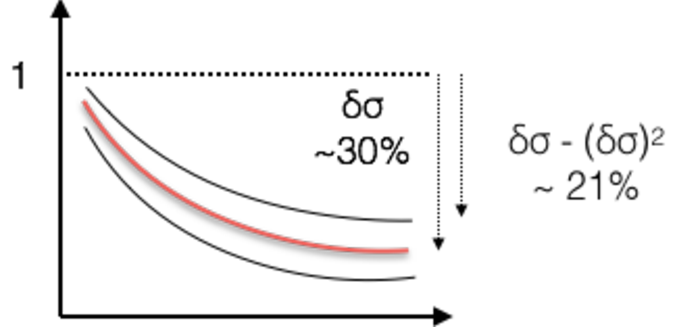
\includegraphics[height=0.3\textwidth]{Analysis/Figures/ewkcorr/scale.pdf}
  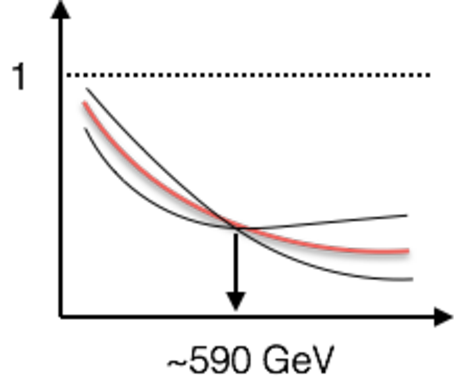
\includegraphics[height=0.3\textwidth]{Analysis/Figures/ewkcorr/shape.pdf}
  \caption{
    Electroweak correction variation scheme to cover the scale (left) and shape (right) uncertainties.
  }
  \label{fig:ewk_correction_cartoon}
\end{figure}

The PDF uncertainty is evaluated by varying the weight of each event using the weights provided in the NNPDF set, and taking the standard deviation of the resulting \ETg\ distributions. 
This uncertainty is considered fully correlated in the ratio between the \zinvg\ and \wlng\ processes, \ie, the variation of the ratio is bounded by the ratios of the upward and downward variations.

Finally, data-to-simulation correction factors $\rho$ for the lepton identification efficiencies have associated uncertainties that do not cancel when taking ratios between regions defined by different lepton selection requirements.

\subsection{Data-driven Control Regions}
\label{sec:control_regions}

Contributions from the \zinvg\ and \wlng\ processes are estimated using observed data in four mutually exclusive single-electron, single-muon, dielectron, and dimuon control regions defined in Section~\ref{sec:event_selection}. 
The ratios between the expected yields of these processes are constrained by MC simulations of \vg\ processes. This background estimation method exploits cancellation of some of the systematic uncertainties, both experimental and theoretical, in the ratios of the photon \ETg\ distributions of \vg\ processes, from here on referred to as ``transfer factors''.
 
For example, in the transfer factor between the \zinvg\ and \zllg\ processes, denoted \RZll, the uncertainties due to photon energy calibration, jet energy resolution, and higher-order QCD effects are significantly reduced compared to when such effects are considered for individual processes. 
The only uncertainties in the transfer factor \RZll\ that do not largely cancel are those on lepton identification efficiency and the statistical uncertainty due to the limited MC sample size. 
Figure~\ref{fig:tf_z} shows the transfer factor \RZee\ (\RZmm) between the dielectron (dimuon) control region and the combined signal regions, for which the numerator is the expected \zinvg\ yield in the combined signal regions and the denominator is the expected \zllg\ yield in the relevant control region.

\begin{figure}[htbp]
  \centering
    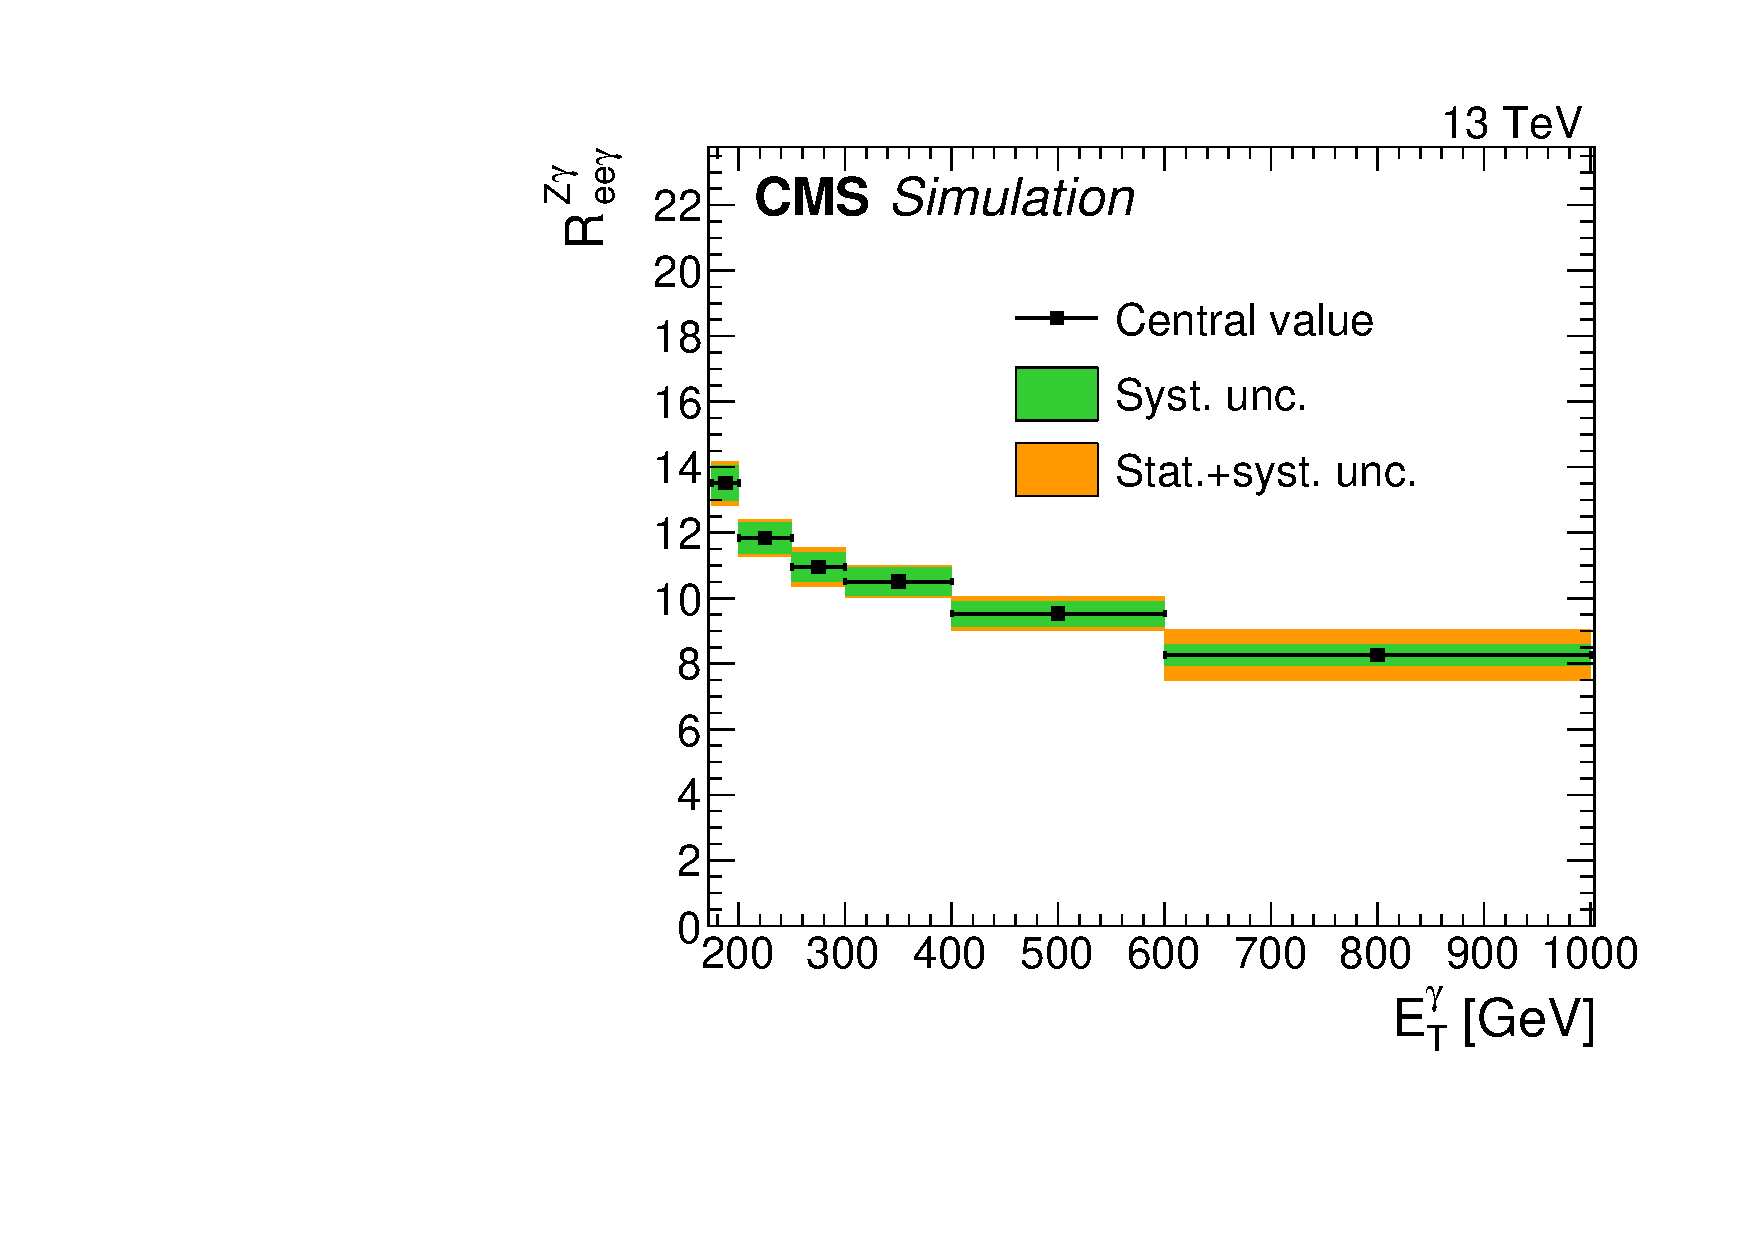
\includegraphics[width=0.49\textwidth]{Analysis/Figures/RZee.pdf}
    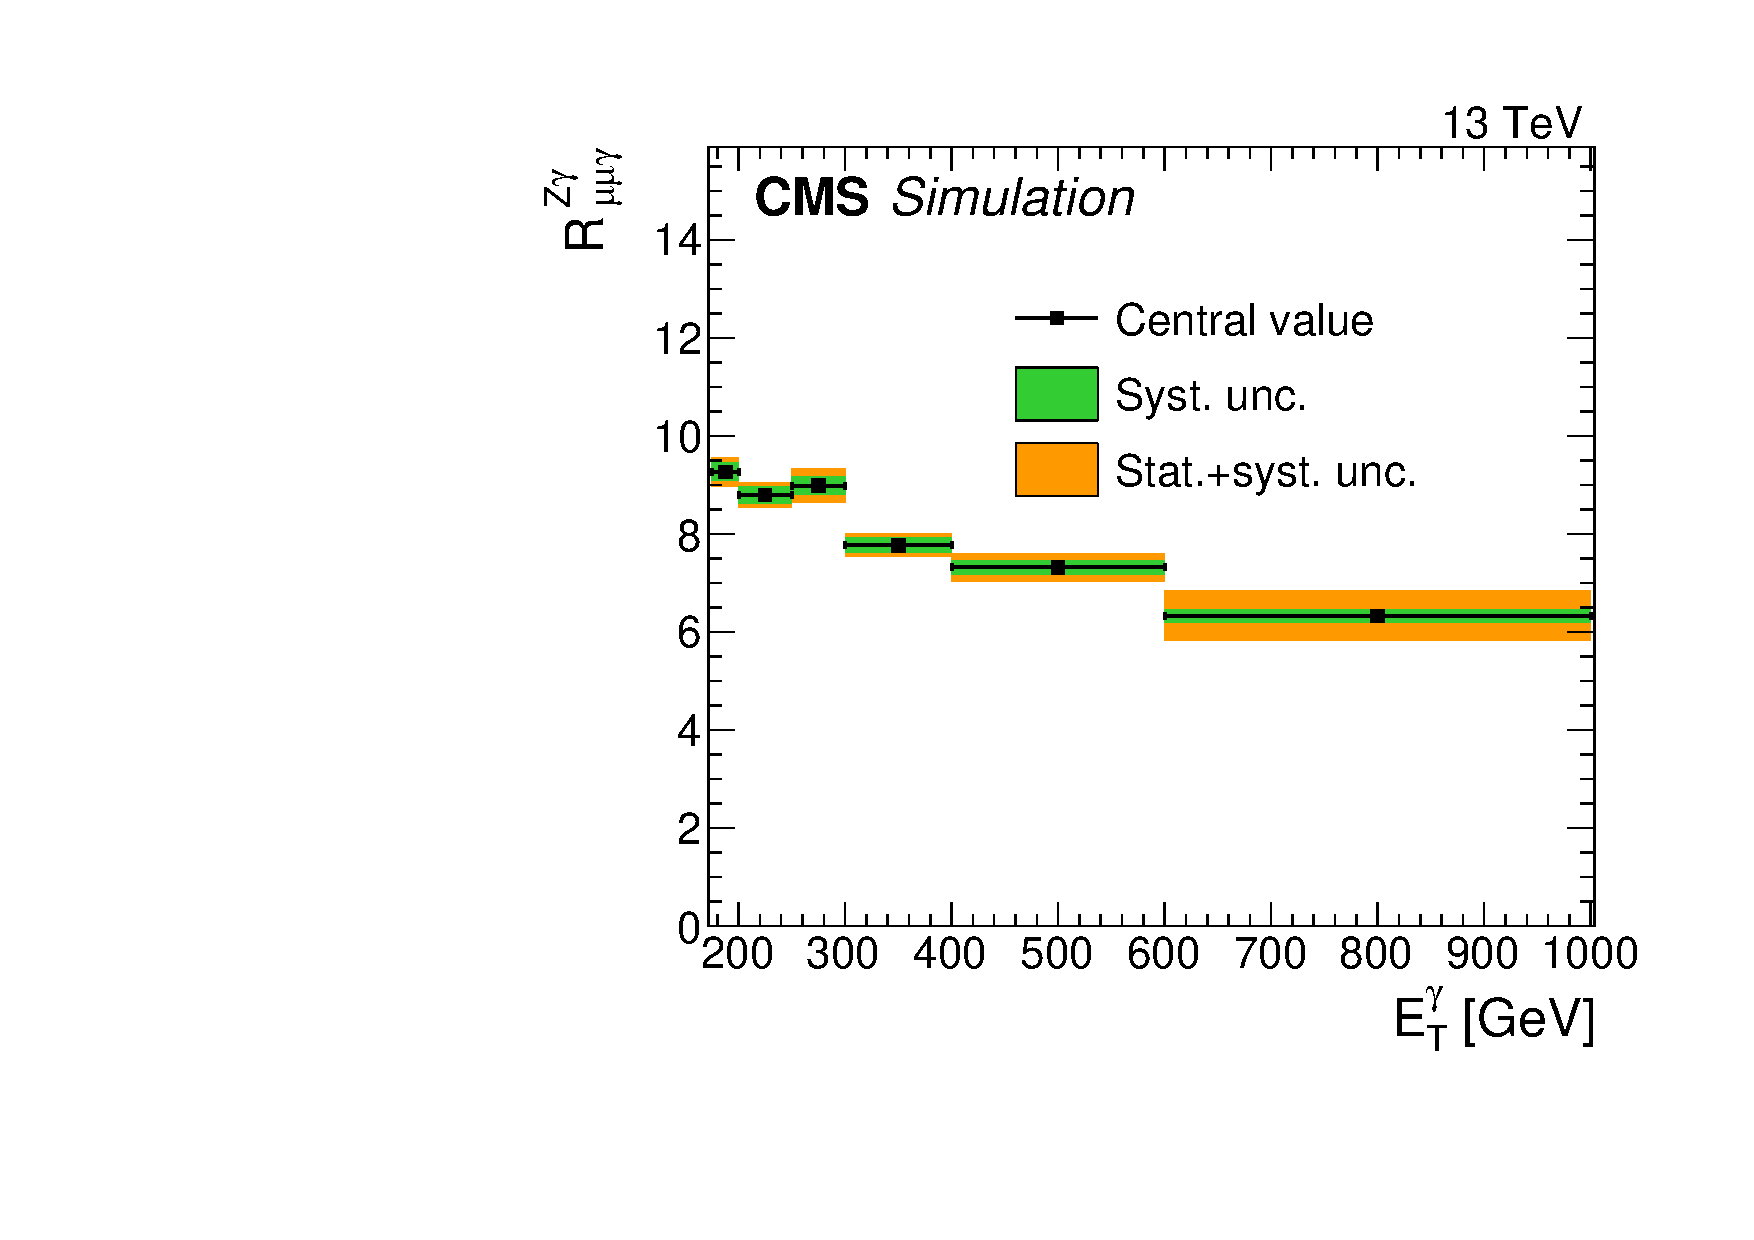
\includegraphics[width=0.49\textwidth]{Analysis/Figures/RZmm.pdf}
    \caption{
      Transfer factors \RZee\ (left) and \RZmm\ (right). 
      The uncertainty bands in green (inner) and orange (outer) show the systematic uncertainty, and the combination of systematic and statistical uncertainty arising from limited MC sample size, respectively. 
      The systematic uncertainties considered are the uncertainties in the data-to-simulation correction factors $\rho$ for the lepton identification efficiencies.
    }
    \label{fig:tf_z}
\end{figure}

For increasing \ETg, the \PZ\ boson in a \zllg\ event tends to emerge with lower rapidity, and hence so do its decay products. 
As a consequence, the charged leptons are more likely to fall within the inner tracker acceptance, which increases the dilepton control region selection efficiency of these events. 
In contrast, the signal region selection efficiency of \zinvg\ events is unafected by the rapidity of the final state neutrinos, as long as the observed \met\ has the appropriate magnitude and azimuthal direction. 
This causes the distinctive drop in the ratio \RZll\ with increasing \ETg.

Using the transfer factor \RZll, the total estimated event yield \Tll\ in each dilepton control region in the $i^\mathrm{th}$ bin of the \ETg\ distribution can be expressed as
\begin{equation}
  \Tll[,i] = \frac{\NZg[i]}{\RZll[,i]} + b_{\ell\ell\Pgg,i},
\end{equation}
where \NZg\ is the number of \zinvg\ events in the combined signal regions and $b_{\ell\ell\Pgg}$ is the predicted contribution from other background sources in the dilepton control region, namely \ttg, VV\Pgg, and misidentified hadrons. 
The subscript $i$ indicates that the quantities are evaluated in bin $i$ of the \ETg\ distribution.

Similar considerations apply to events arising from \wlng\ processes. 
A large fraction of such events are rejected by the electron and muon vetoes in the signal region selection and end up in the control regions instead. 
However, hadronic tau events and events where the leptons are out of acceptance or fail to be reconstructed will remain in the signal region, on top of the vetoes having imperfect efficiencies. 
In the ratio of these two classes of events, denoted \RWl, the only uncertainties that remain non-negligible are those associated with the lepton identification efficiency and the MC statistical uncertainty.

Table~\ref{tab:wg_breakdown} gives the breakdown of the \wlng\ background passing the full event selection for the signal region, categorized by the lepton flavor and, for the case of electrons and muons, the lepton pseudorapidity at the parton-level. 
From this breakdown, one sees that events where the \PW\ boson decays to a \Pgt\ and a neutrino constitutes approximately 60\% of the \wlng\ background. 
The remaining 40\% of the \wlng\ background comes from events where \PW\ boson decays to a \Pgm\ or \Pe\ and a neutrino.
Events containing an electron are more likely to be within the detector acceptance, while those with a muon are more likely to be out of acceptance.
For the in-acceptance background ($|\eta| < 2.5$), the identification efficiency, which is lower for electrons than for muons, which translates to a larger background contribution from the electrons. 
Meanwhile, the \met requirement explains the behavior of the out-of-acceptance background ($\abs\eta > 2.5$).
A large fraction of electrons that are out of tracker acceptance are still captured by the calorimeters, while out-of-acceptance muons directly contribute to missing momentum leading to a larger background contribution from muons.
% Conversely, by requiring large \met, the muon $\eta$ distribution is highly skewed towards the edge of acceptance, driving the overall muon reconstruction efficiency in the sample lower and thereby making the background contributions from electrons and muons closer to each other. 

\begin{table}[tbp]
  \begin{center}
    \begin{tabular}{ l r | r r }
      \multicolumn{2}{ c |}{Subprocess} & \multicolumn{2}{| c }{$A\times\epsilon \times 10^{3}$} \\
      \hline
      \multicolumn{2}{ l |}{$\PW\rightarrow\Pe\Pgn + \Pgg$} & 1.68 & \\
      & $|\eta^{\Pe}| < 2.5$ & & 1.35 \\
      & $|\eta^{\Pe}| > 2.5$ & & 0.32 \\
      \hline
      \multicolumn{2}{ l |}{$\PW\rightarrow\Pgm\Pgn + \Pgg$} & 1.83 & \\
      & $|\eta^{\Pgm} < 2.5$ & & 0.74 \\
      & $|\eta^{\Pgm} > 2.5$ & & 1.08 \\
      \hline
      \multicolumn{2}{ l |}{$\PW\rightarrow\Pgt\Pgn + \Pgg$} & 5.03 & \\
    \end{tabular}
    \caption{
      The breakdown of simulated $\PW+\Pgg$ events passing the full event selection. 
      Events are categorized in the \PW\ decay mode. 
      Events with \Pe\Pgn\ and \Pgm\Pgn\ final states are further divided into those where the lepton was roughly within acceptance ($|\eta| < 2.5$) but failed the lepton veto, and those where the lepton was out of acceptance ($|\eta| > 2.5$). 
      For each \PW\ decay mode, the fraction out of total generated ($A\times\epsilon$) is shown.
    }
    \label{tab:wg_breakdown}
  \end{center}
\end{table}


Figure~\ref{fig:tf_w} shows the transfer factor \RWe\ (\RWm) between the single-electron (single-muon) control region and the combined signal regions, for which the numerator is the estimated \wlng\ yield in the combined signal regions, and the denominator is the estimated \wlng\ yield in the relevant control region. 
The ratio \RWl\ decreases with increasing \ETg\ in a similar manner to \RZll.
The underlying logic is the same; e.g., that the signal region selection efficiency is unaffected by \ETg\ while the control region acceptances increase with increasing \ETg\ due to increased lepton efficiency resulting from lower \PW\ rapidity. 

\begin{figure}[htbp]
  \centering
    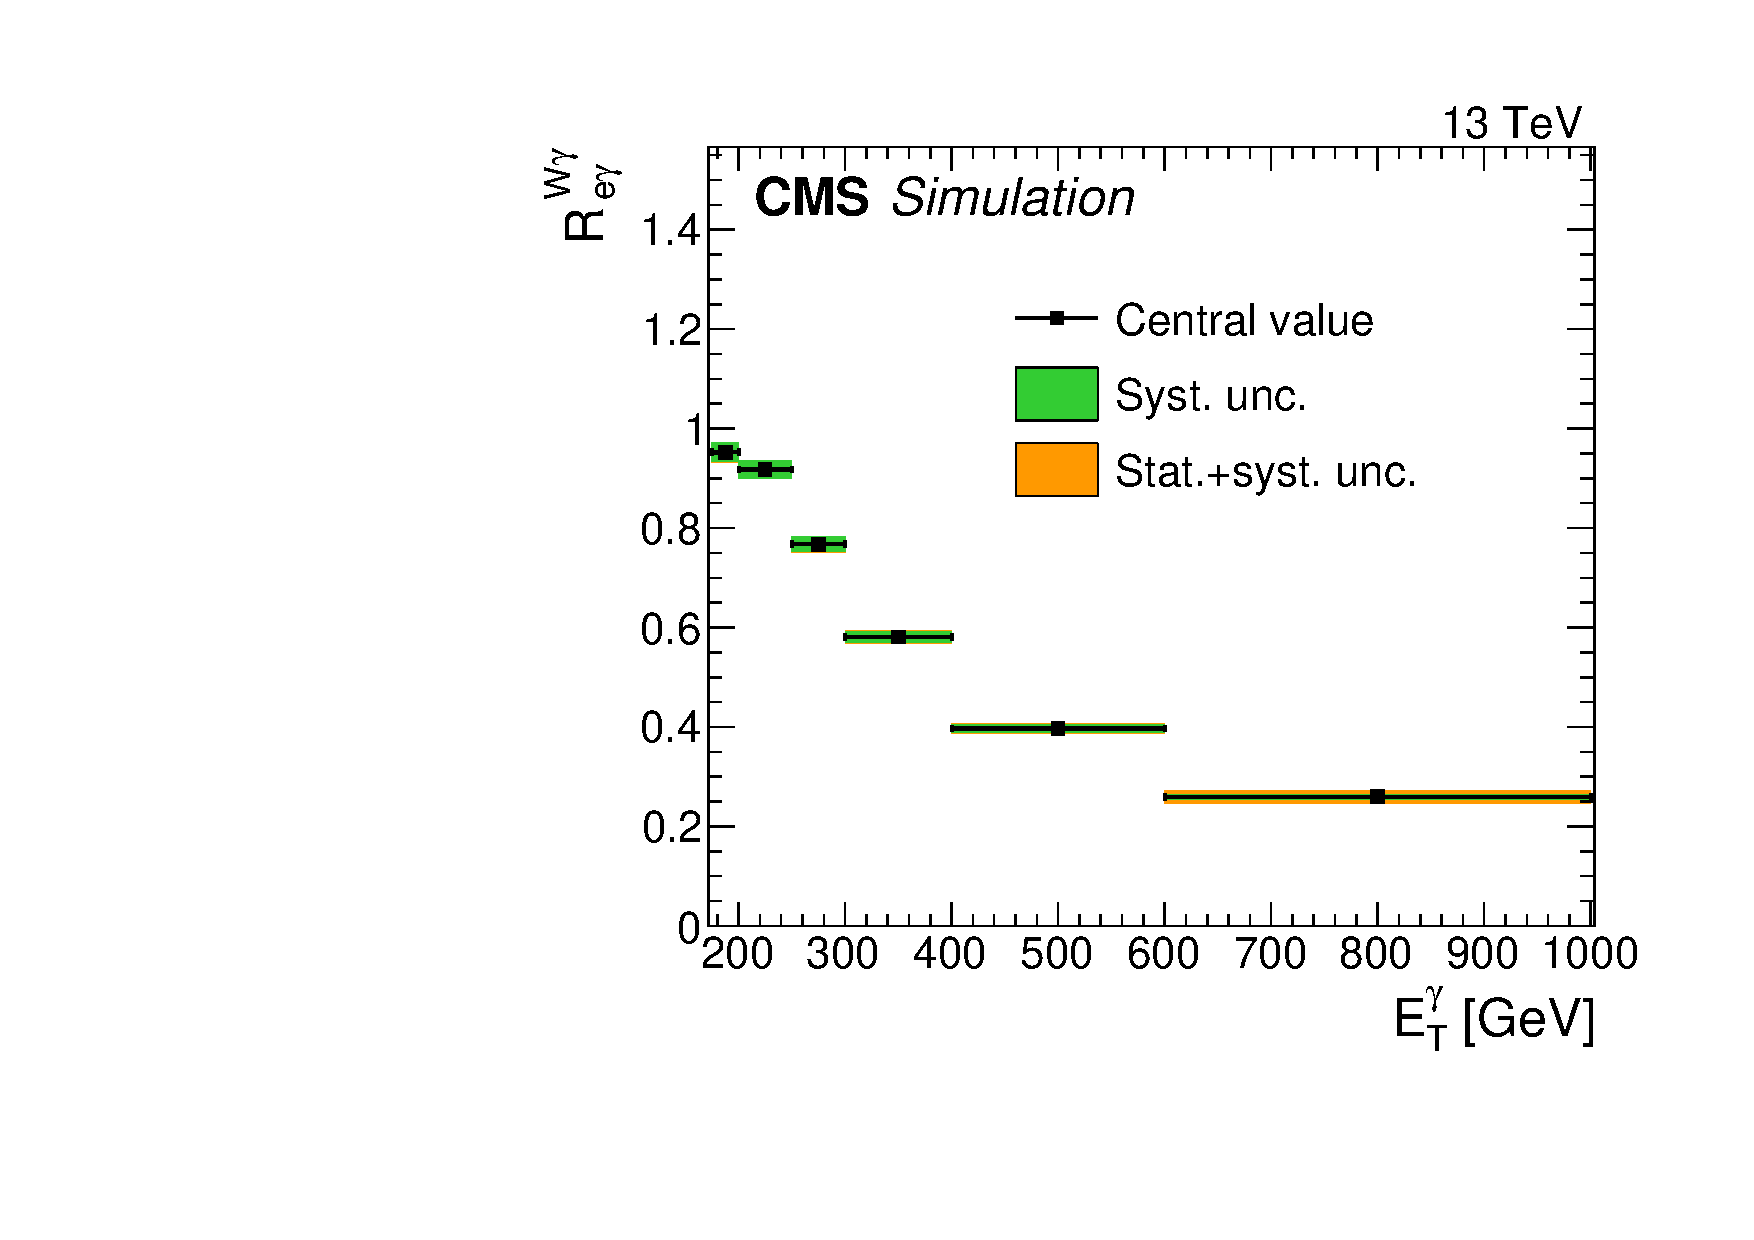
\includegraphics[width=0.49\textwidth]{Analysis/Figures/RWe.pdf}
    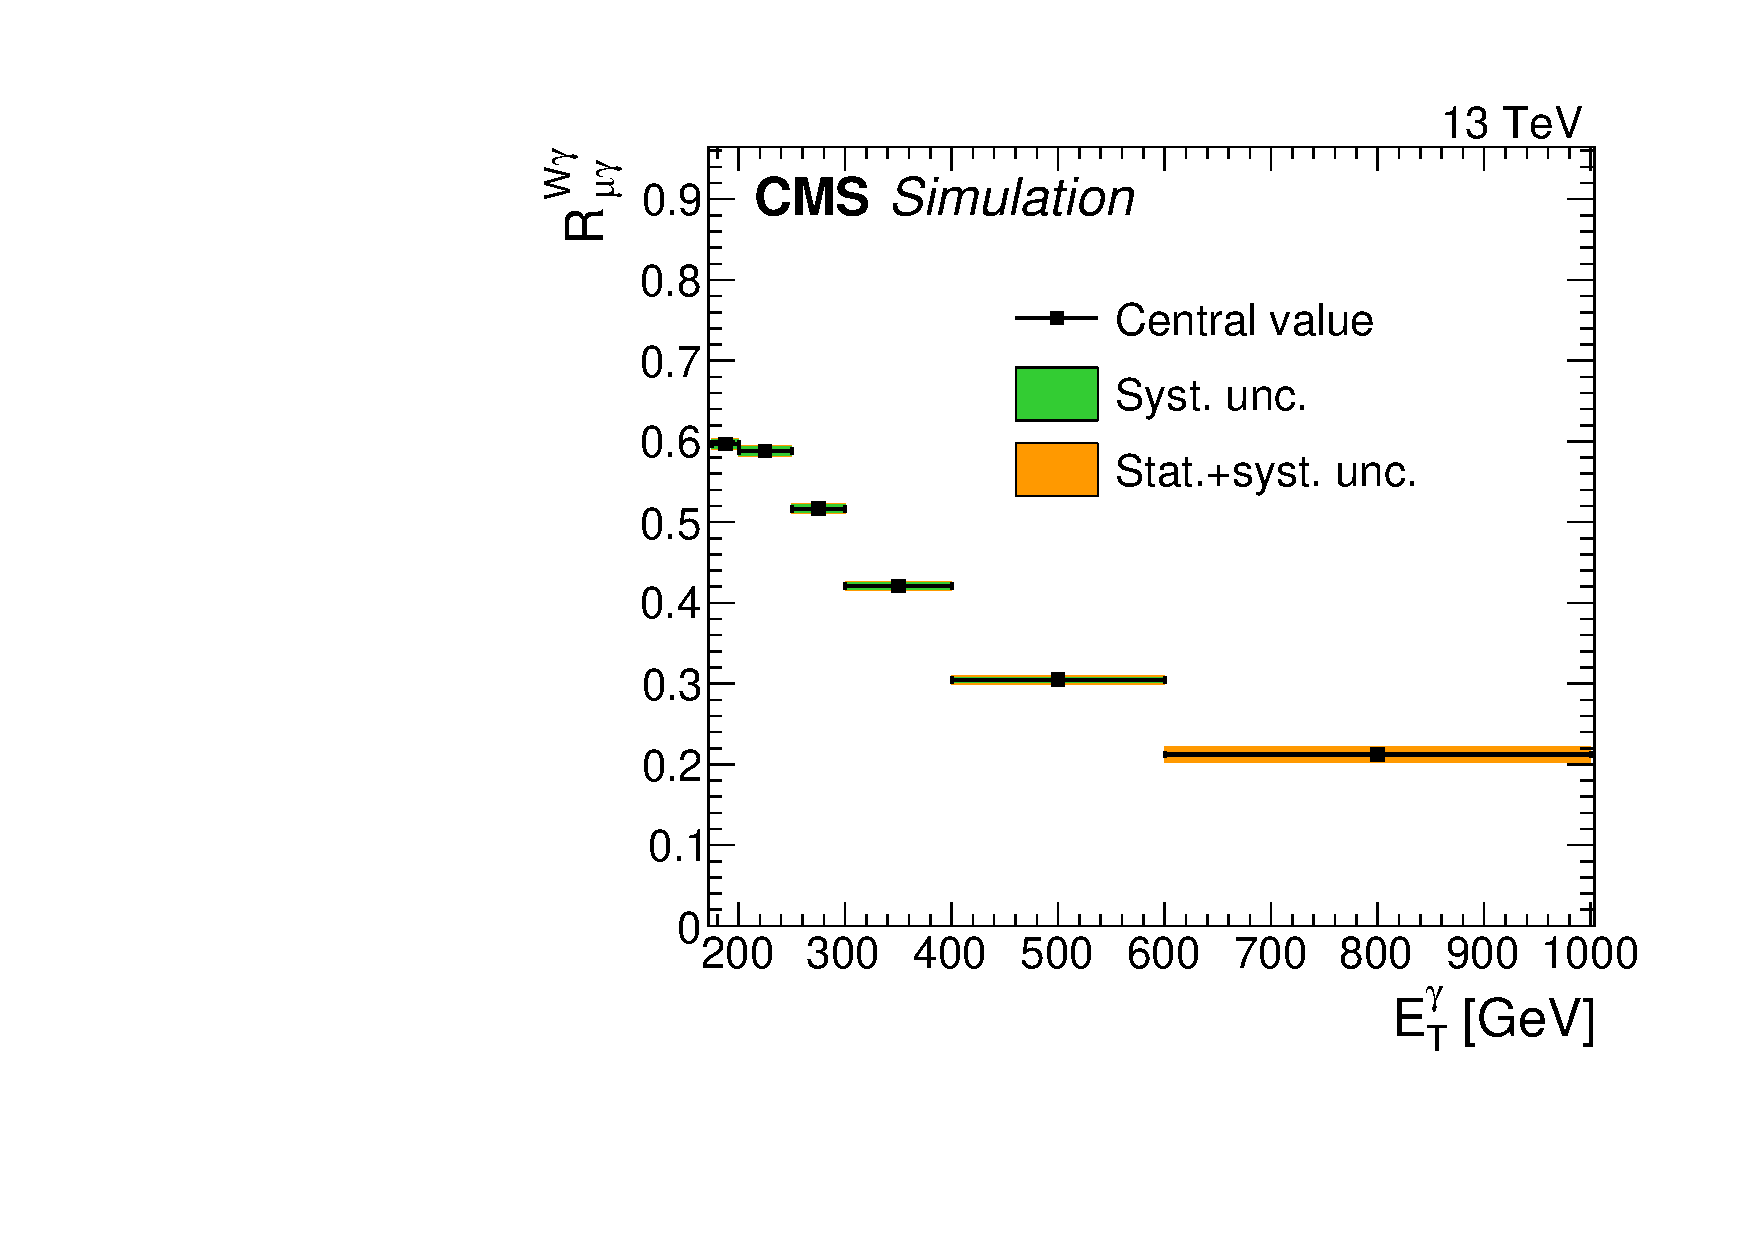
\includegraphics[width=0.49\textwidth]{Analysis/Figures/RWm.pdf}
    \caption{
      Transfer factors \RWe\ (left) and \RWm\ (right). 
      The uncertainty bands in green (inner) and orange (outer) show the systematic uncertainty, and the combination of systematic and statistical uncertainty arising from limited MC sample size, respectively. 
      The systematic uncertainties considered are the uncertainties in the data-to-simulation correction factors $\rho$ for the lepton identification efficiencies.
    }
    \label{fig:tf_w}
\end{figure}

Finally, to benefit further from the larger statistical power that the single-lepton control samples provides, an additional transfer factor $\fZW = \NZg / \NWg$ is defined to connect the \zinvg\ and \wlng\ background yields in the signal regions, where the quantity $\NWg$ is the number of \wlng\ events in the combined signal regions. 
When calculating the ratio \fZW, all experimental uncertainties associated with the data-to-simulation correction factors $\rho$ cancel since both processes result in very similar event configurations. 
The main uncertainties in \fZW\ are those from higher-order theoretical corrections, discussed in Section~\ref{sec:vgmc}. Figure~\ref{fig:tf_syst} shows the effect of each systematic uncertainty in \fZW\ with respects to its nominal value for \zinvg\ and \wlng\ respectively.

\begin{figure}[htbp]
  \centering
    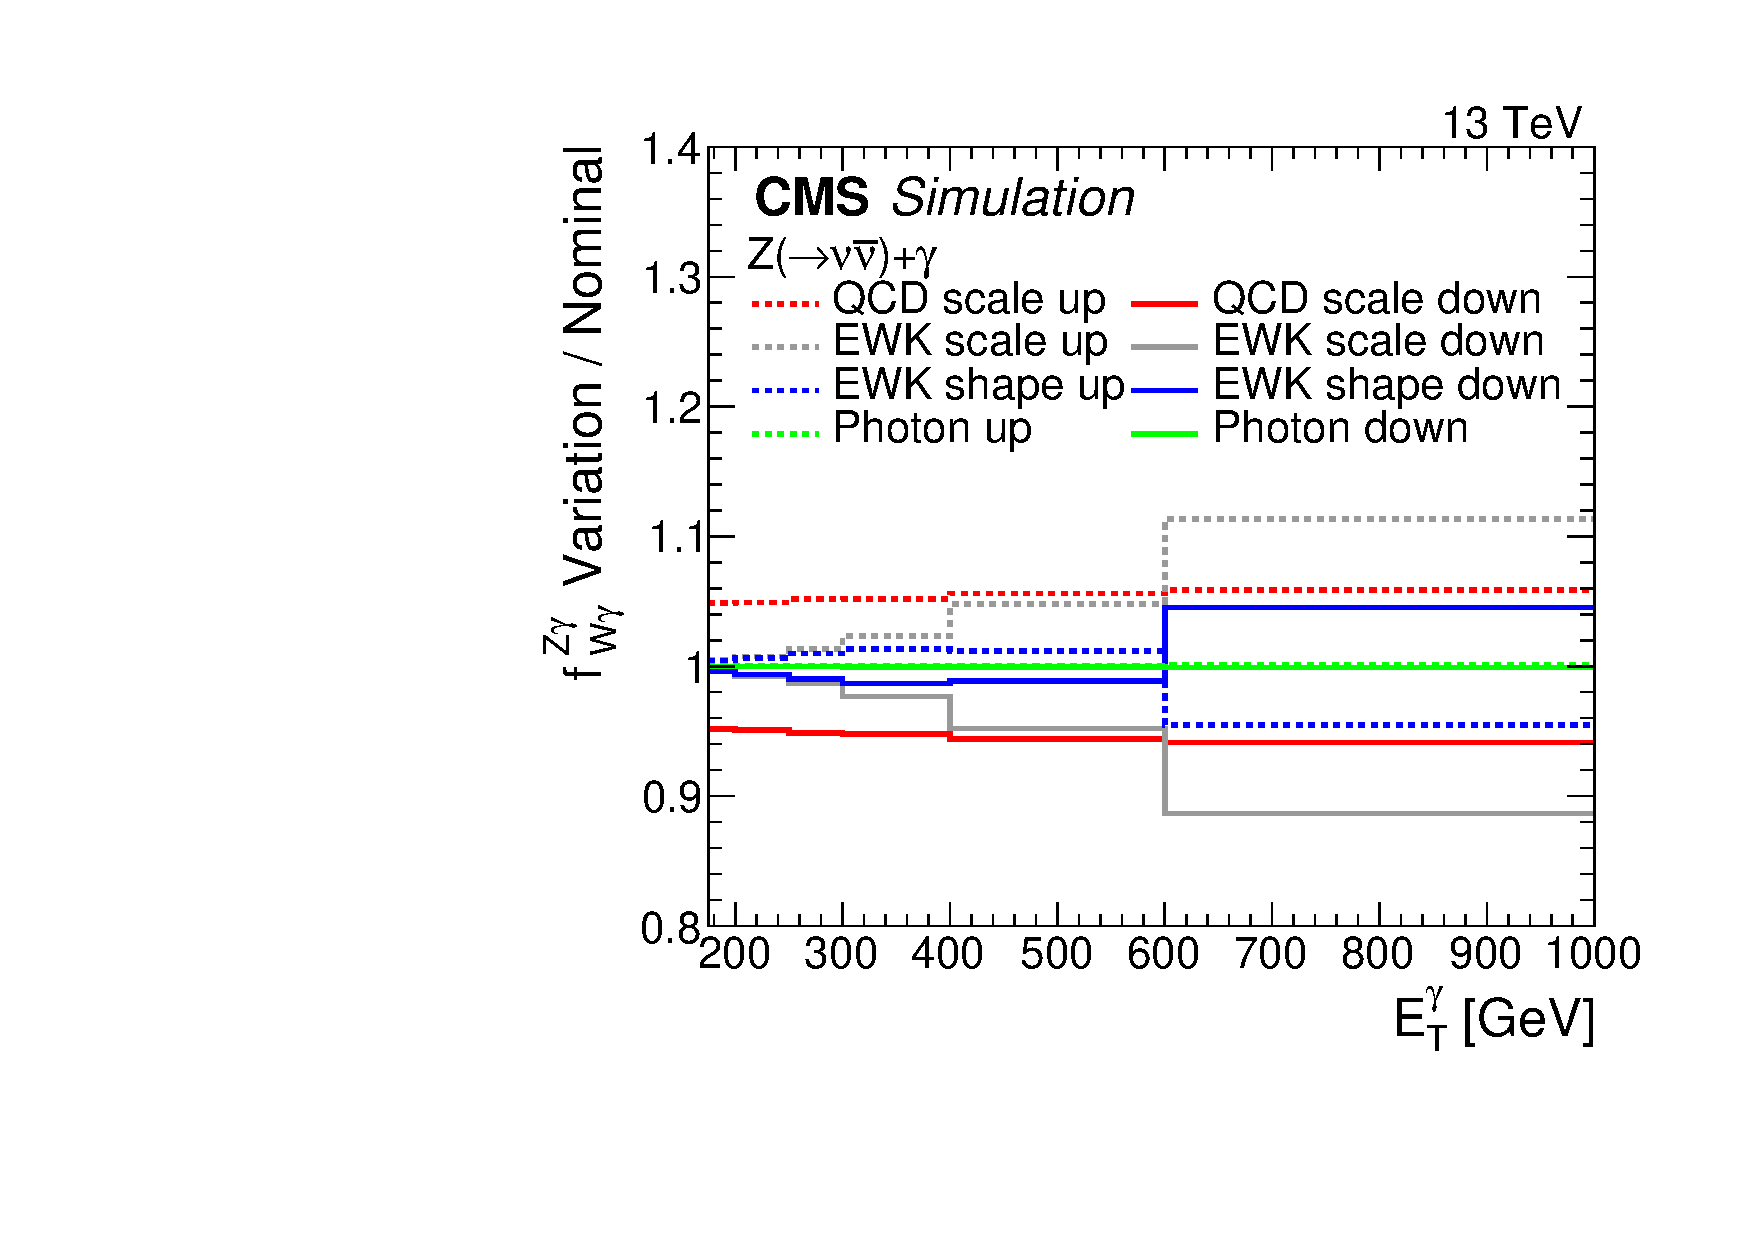
\includegraphics[width=0.49\textwidth]{Analysis/Figures/tf_syst_zg.pdf}
    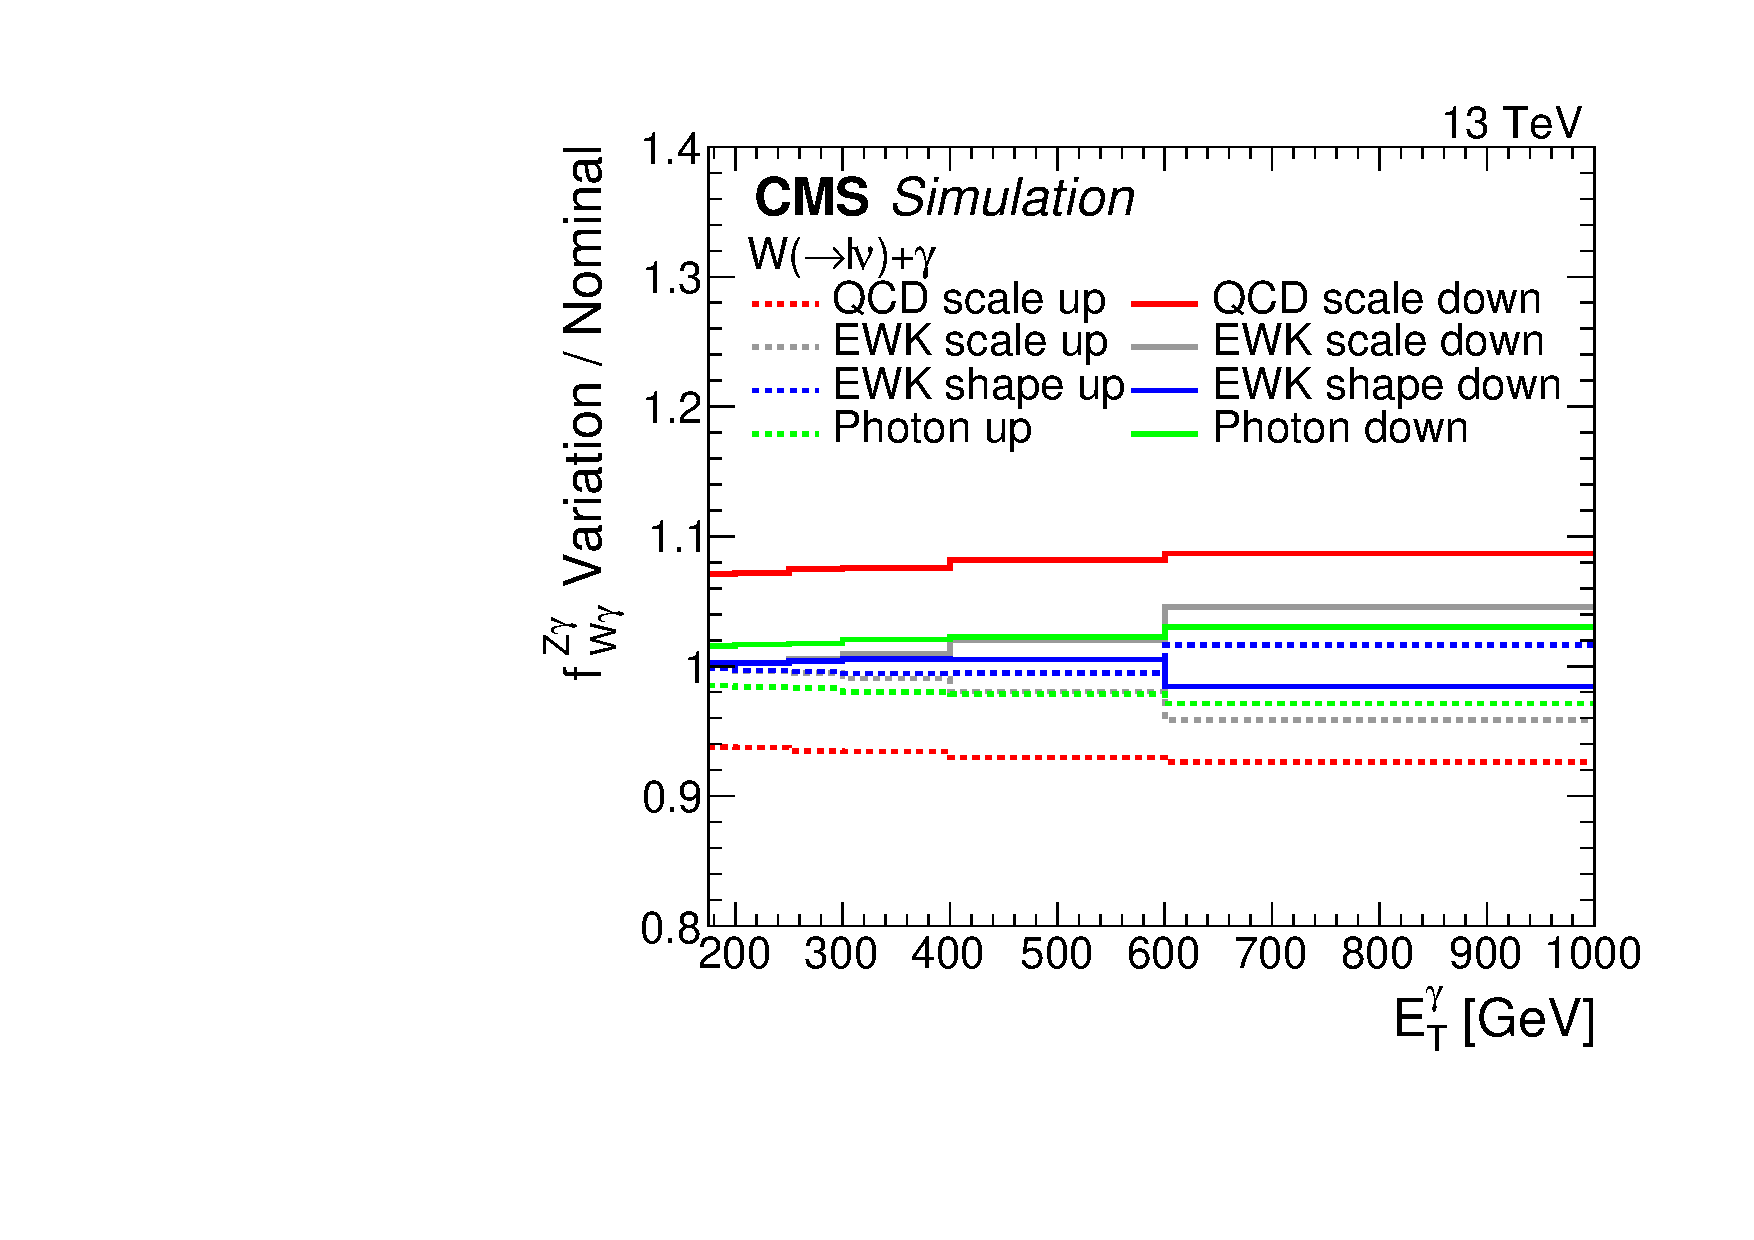
\includegraphics[width=0.49\textwidth]{Analysis/Figures/tf_syst_wg.pdf}
    \caption{
      Systematic uncertainty in the transfer factors for \zinvg\ (left) and \wlng\ (right). The last bin includes all events with $\ETg > 1000\GeV$.
    }
    \label{fig:tf_syst}
\end{figure}

The ratio \fZW\ rises rather than falls with increasing \ETg\ because \wlng\ events have a lower rather than higher signal region selection efficiency if the charged lepton falls within the tracker acceptance while the \zinvg\ efficiency is independent of \ETg. Figure~\ref{fig:tf_wz} shows the transfer factor \fZW\ between the \zinvg\ and \wlng\ processes in the combined signal region.


\begin{figure}[htbp]
  \centering
    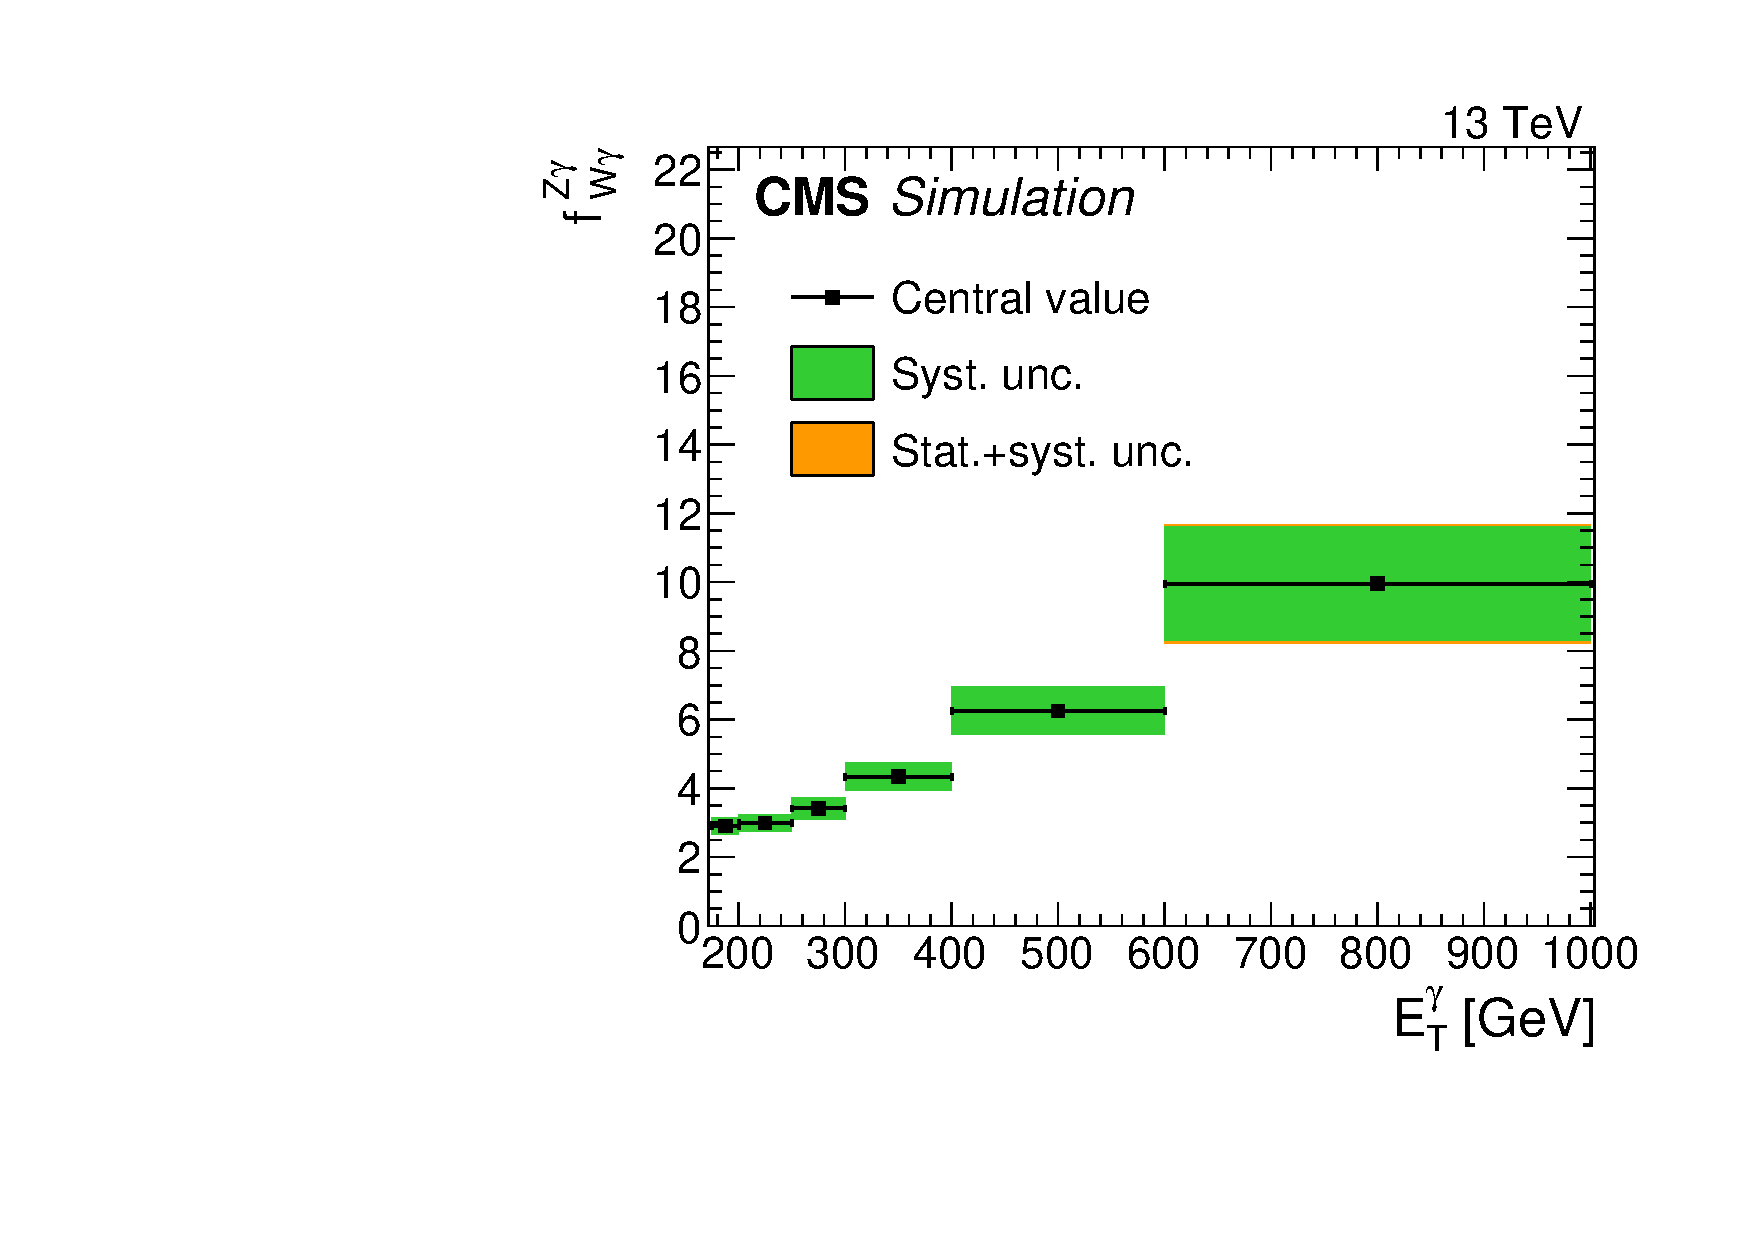
\includegraphics[width=0.49\textwidth]{Analysis/Figures/fZW.pdf}
    \caption{
      Transfer factor \fZW. 
      The uncertainty bands in green (inner) and orange (outer) show the systematic uncertainty, and the combination of systematic and statistical uncertainty arising from limited MC sample size, respectively. 
      The systematic uncertainties considered are the uncertainties from higher-order theoretical corrections.
    }
    \label{fig:tf_wz}
\end{figure}

Using \RWl\ and \fZW, the total estimated event yield \Tl\ in each single-lepton control region in the $i^\mathrm{th}$ bin of the \ETg\ distribution can be expressed as
\begin{equation}
  \Tl[,i] = \frac{\NZg[i]}{\RWl[,i]\fZW[,i]} + b_{\ell\Pgg,i},
\end{equation}
where $b_{\ell\Pgg}$ is the predicted contribution from other background sources in the single-lepton regions, namely misidentified electrons and hadrons and other minor SM processes.

\section{Misidentified electrons}
\label{sec:efake}

An electron can be misidentified as a photon if the association of tracks or track seeds to the supercluster in ECAL fails in the reconstruction step. 
The production of a single \PW\ boson decaying to an electron and a neutrino is a high-rate process, and it mimicks the photon plus \met\ signature if the electron is misidentified.

The rate at which this misidentification occurs is proportional to the inefficiency $1 - \epsilon_{\Pe}^{\text{track}}$ of the tracking, defined over the electrons passing the photon identification criteria described in Sec.~\ref{sec:pf_photons} except the electron veto. 
This partial identification is denoted as \Pe\Pgg\ ID in the following.  
If one assumes that the kinematic and other critical properties of the electron plus \met\ events are unaffected by the electron misidentification, it is possible to model the electron misidentification background by taking a proxy sample with well-identified electrons and scaling this sample by $R_{\Pe} = (1 - \epsilon_{\Pe}^{\text{track}}) / \epsilon_{\Pe}^{\text{track}}$.

The ``tag-and-probe'' method described in Section~\ref{sec:idsf} with appropriate changes is used to measure the efficiency corresponding to the factor $R_{\Pe}$ in data.

The first such change is that the sample is split into \Pe\Pgg\ and \Pe\Pe\ categories depending on whether the probe passes or fails the electron veto requirement. 
Probes in both categories must also pass the \Pe\Pgg\ ID.
Denoting the area of the peak in each cateogry  $N_{\Pe\Pgg}$ and $N_{\Pe\Pe}$, respectively, the ratio $N_{\Pe\Pgg} / N_{\Pe\Pe}$ is equal to $R_{\Pe}$ up to minor systematic corrections.

The second such change is in the background model used in the TP fits. 
The backgrounds to the \Pe\Pgg\ fit consist of processes with actual electron and photon in the final state, such as \PW\Pgg\ and \Zee\ with a hard radiation off one of the electrons.
Because of this, we scale the mass distrubition of the $\Pgm+\Pgg$ sample by the ratio of electron-probe to muon-probe events taken from MC to account for the different rates of FSR and bremsstrahlung between muons and electrons.
As an alternative template to assess the systematic effect introduced by the choice of the background template, the unscaled mass distribution is also tested.

Figure~\ref{fig:efake_fits} shows the six fits performed on \Pe\Pe\ and \Pe\Pgg\ in bins of probe $\pt$, from which the $R_{\Pe}$ factor used for the estimation of the electron misidentification background is derived. 

%%% these fils have charged PF veto included, need to swap out
\begin{figure}[htbp]
  \begin{center}
    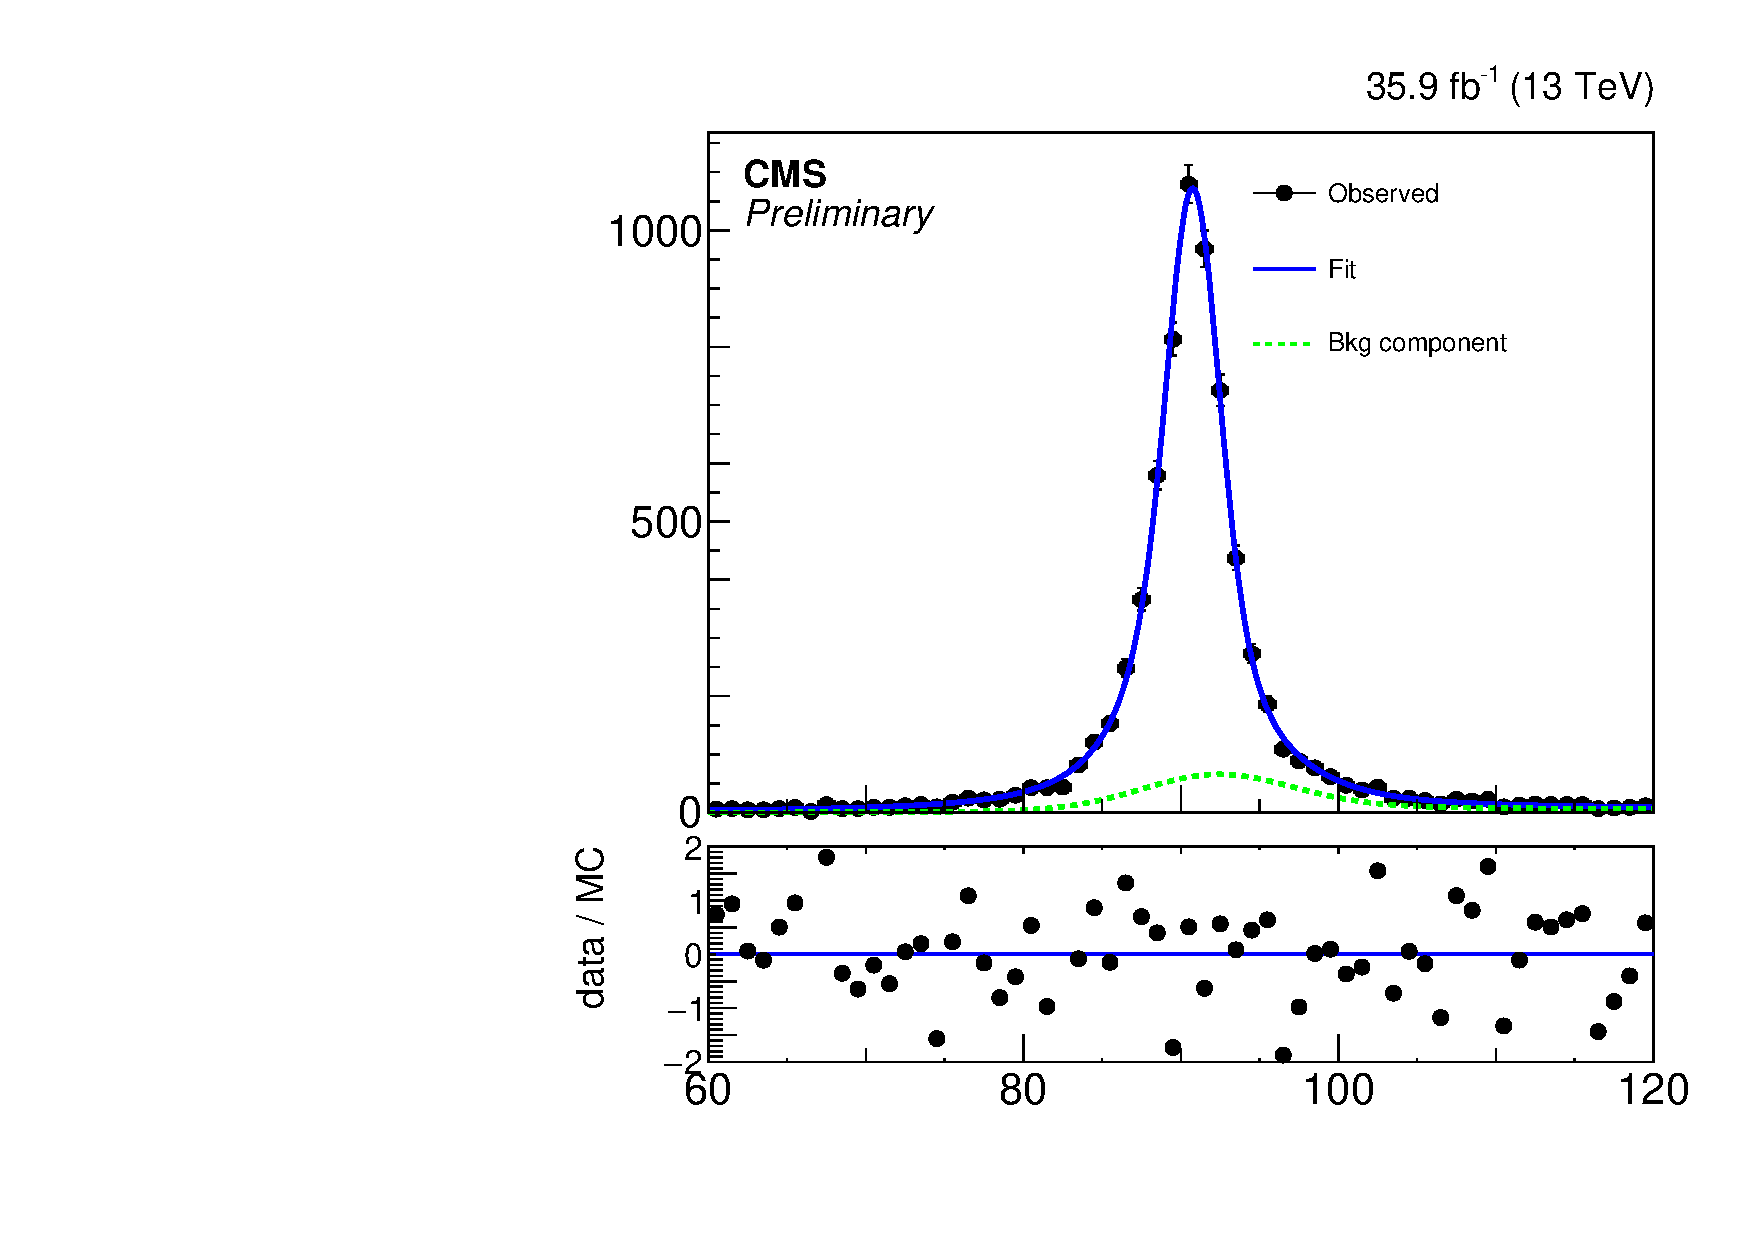
\includegraphics[width=0.47\textwidth]{Analysis/Figures/fit_data_ee_pt_175_200.pdf}
    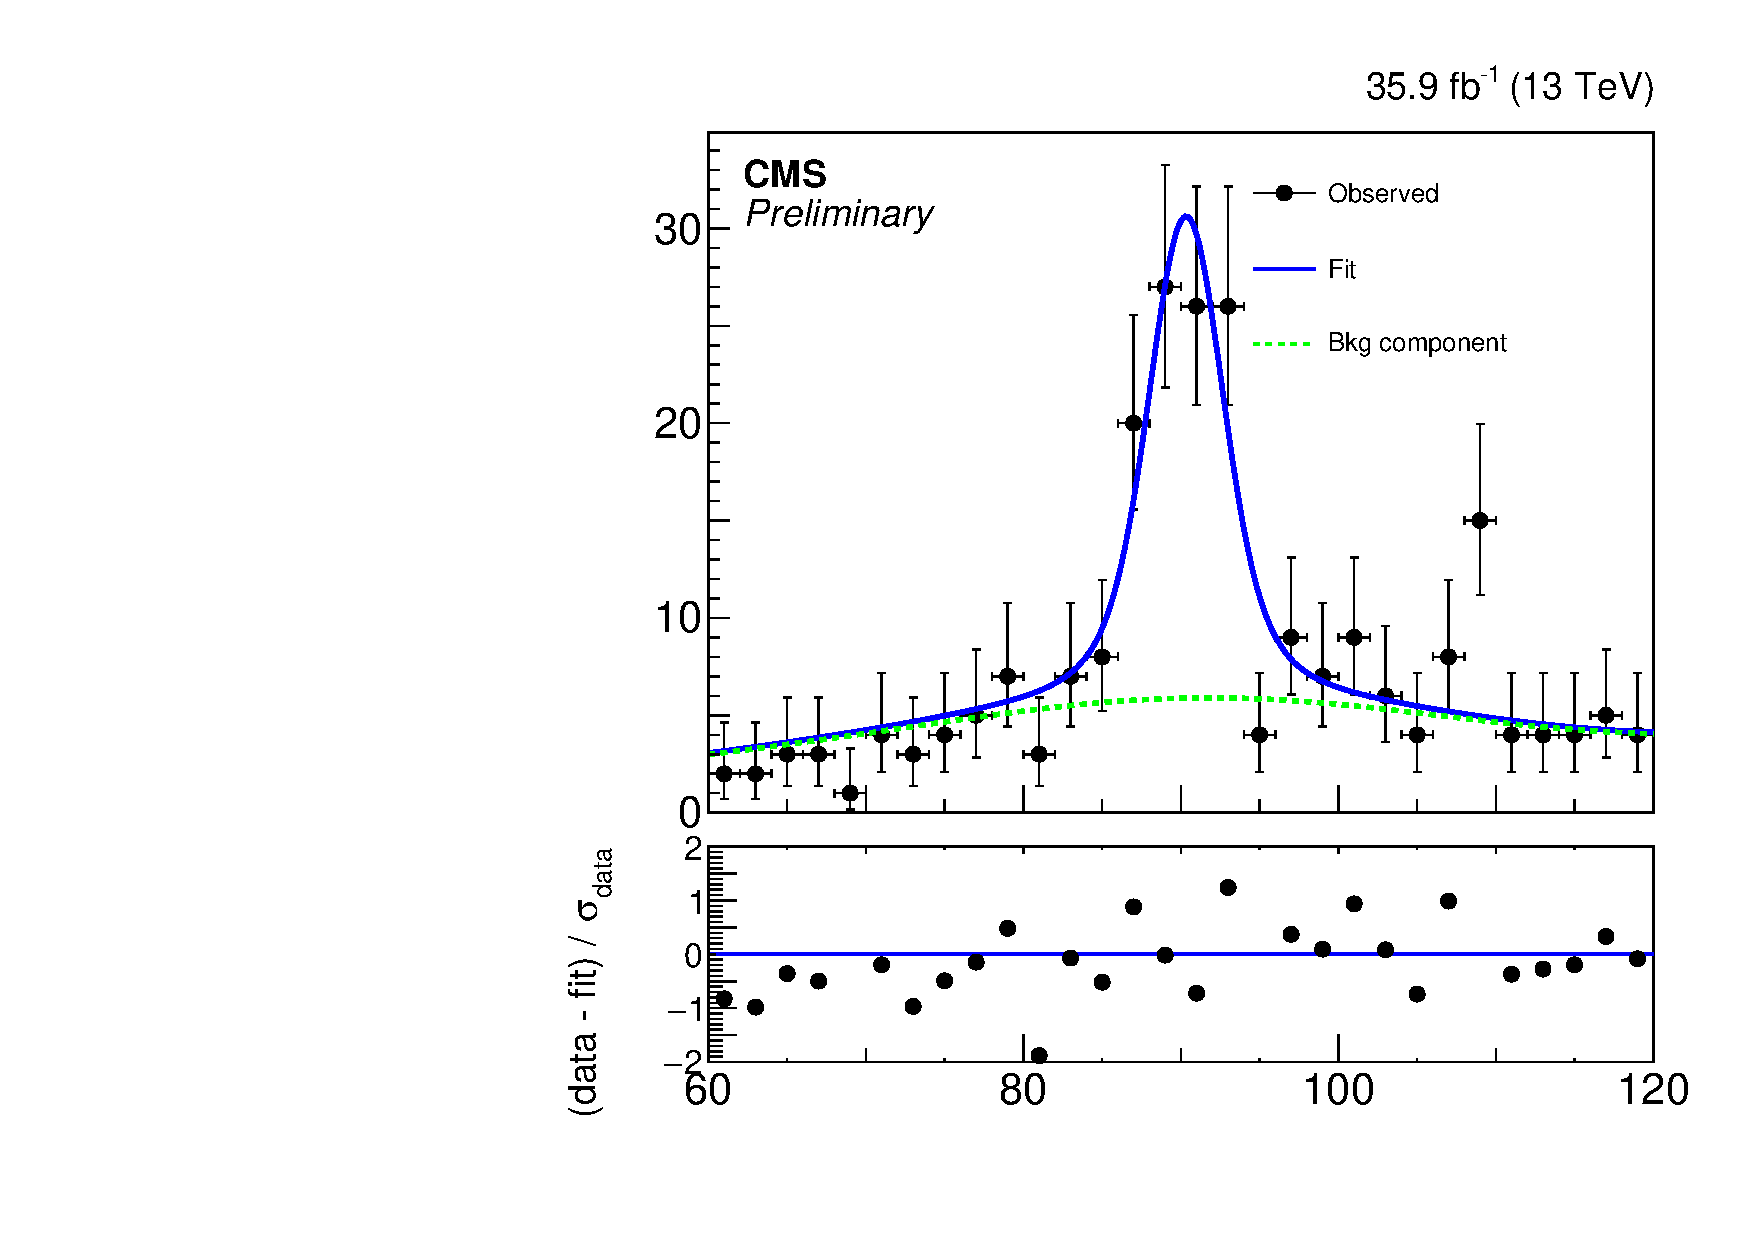
\includegraphics[width=0.47\textwidth]{Analysis/Figures/fit_data_eg_pt_175_200.pdf}
    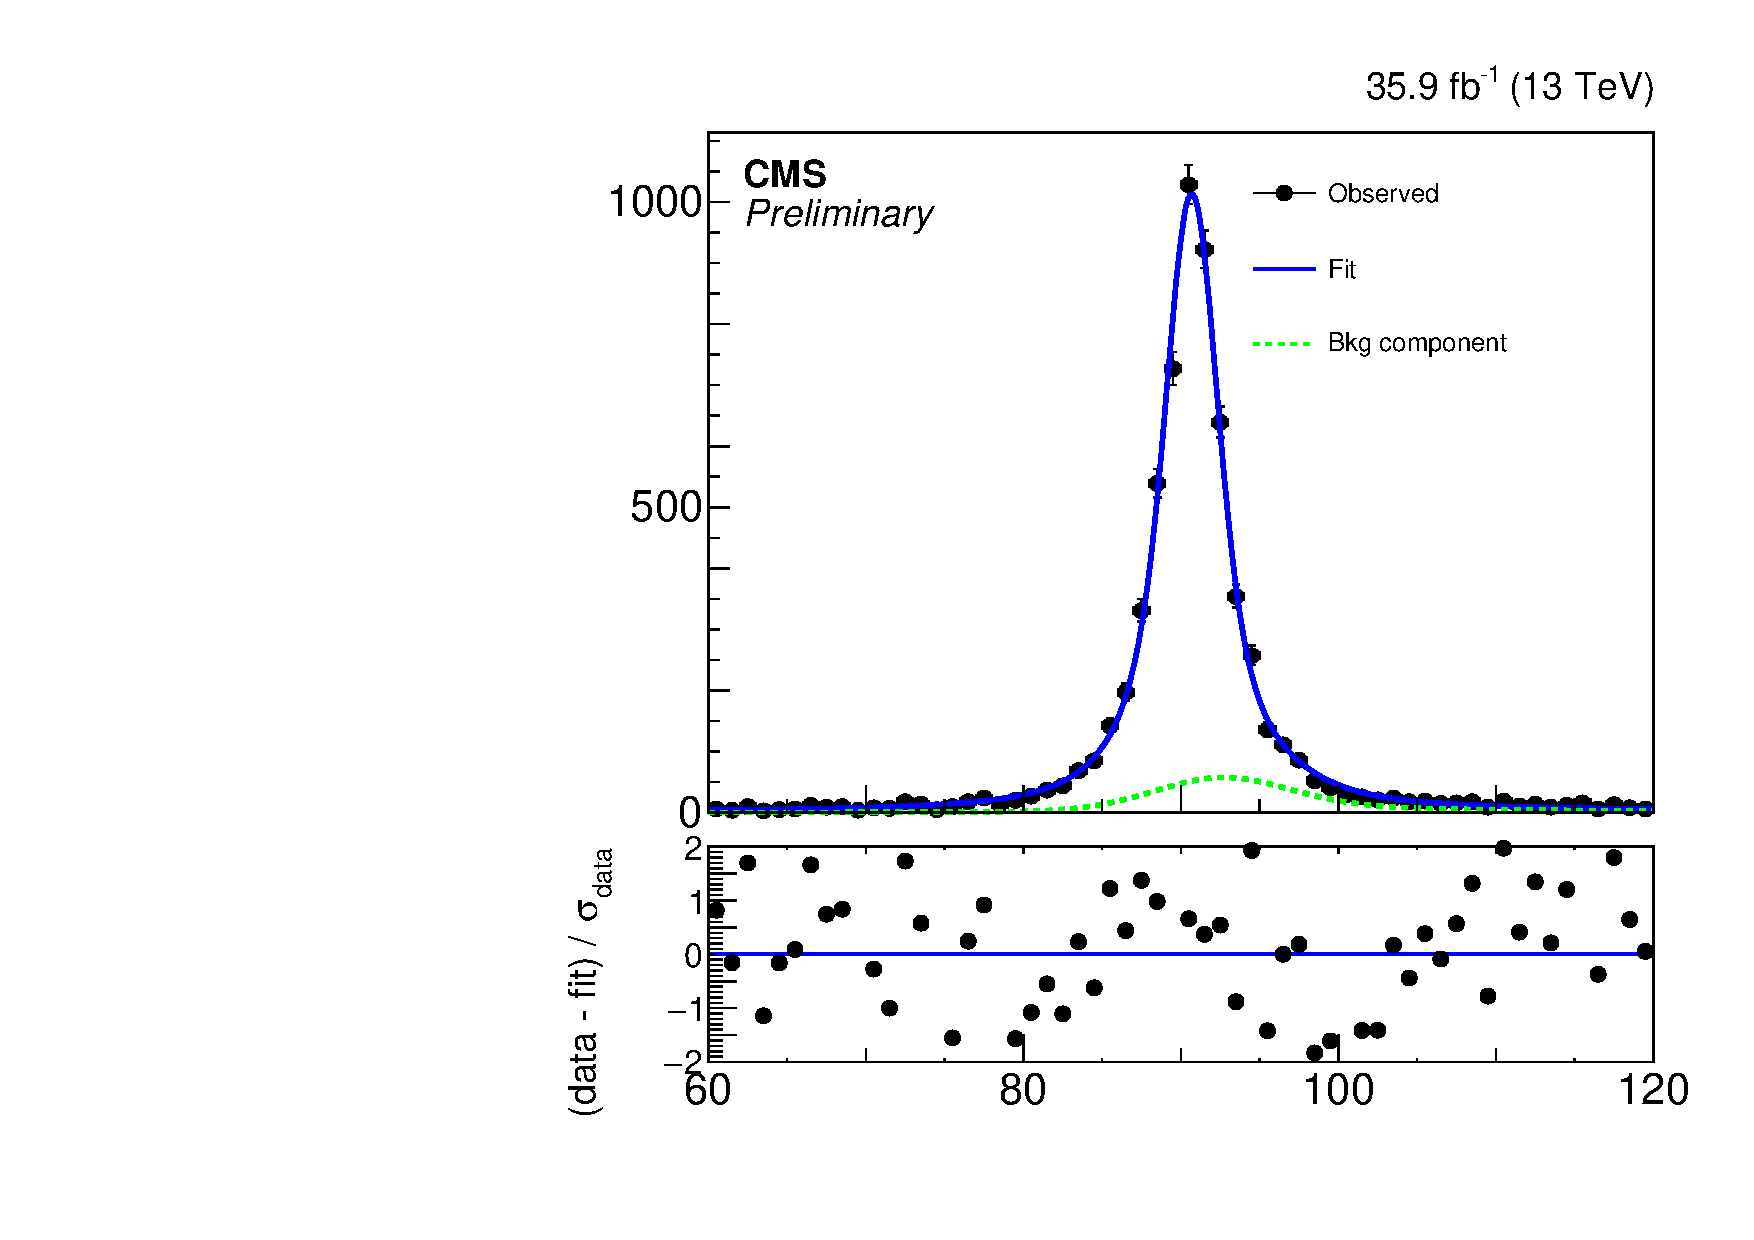
\includegraphics[width=0.47\textwidth]{Analysis/Figures/fit_data_ee_pt_200_250.pdf}
    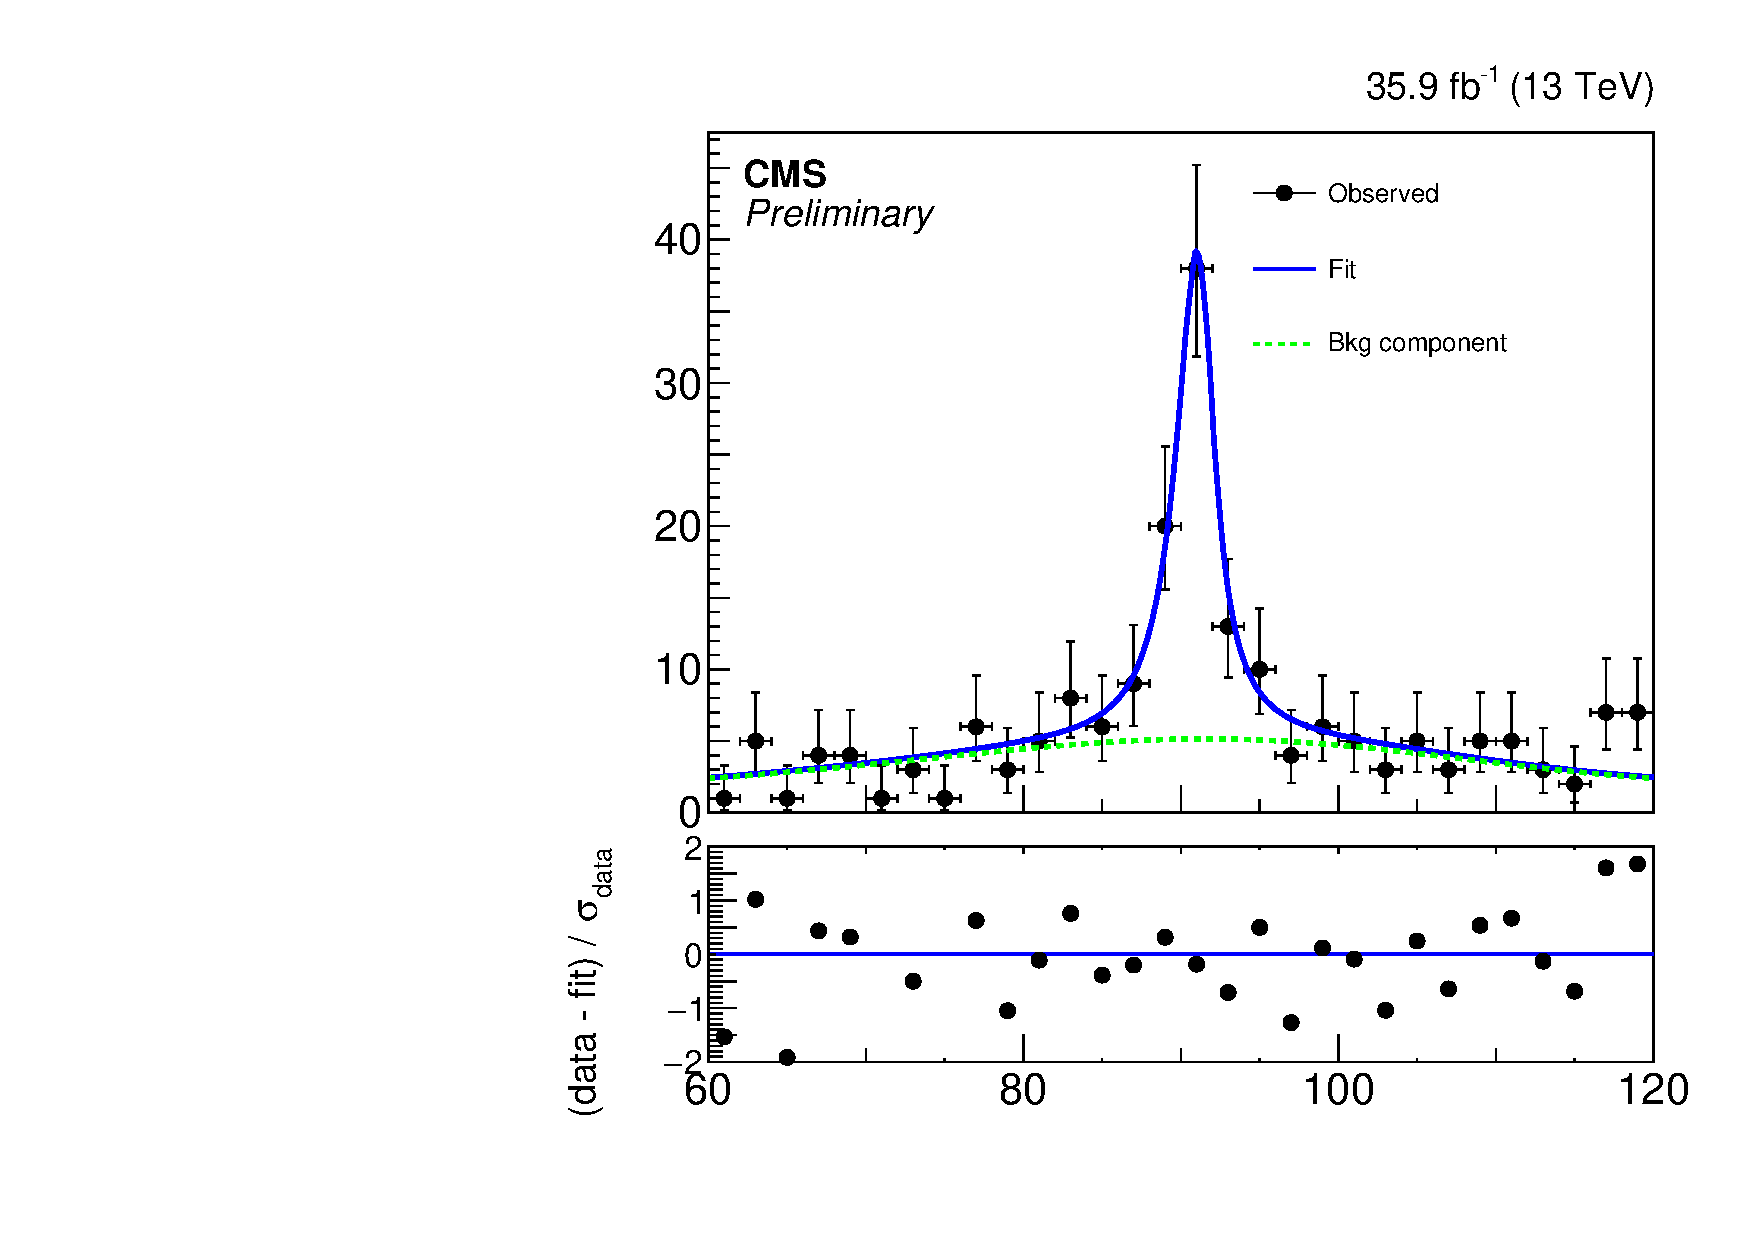
\includegraphics[width=0.47\textwidth]{Analysis/Figures/fit_data_eg_pt_200_250.pdf}
    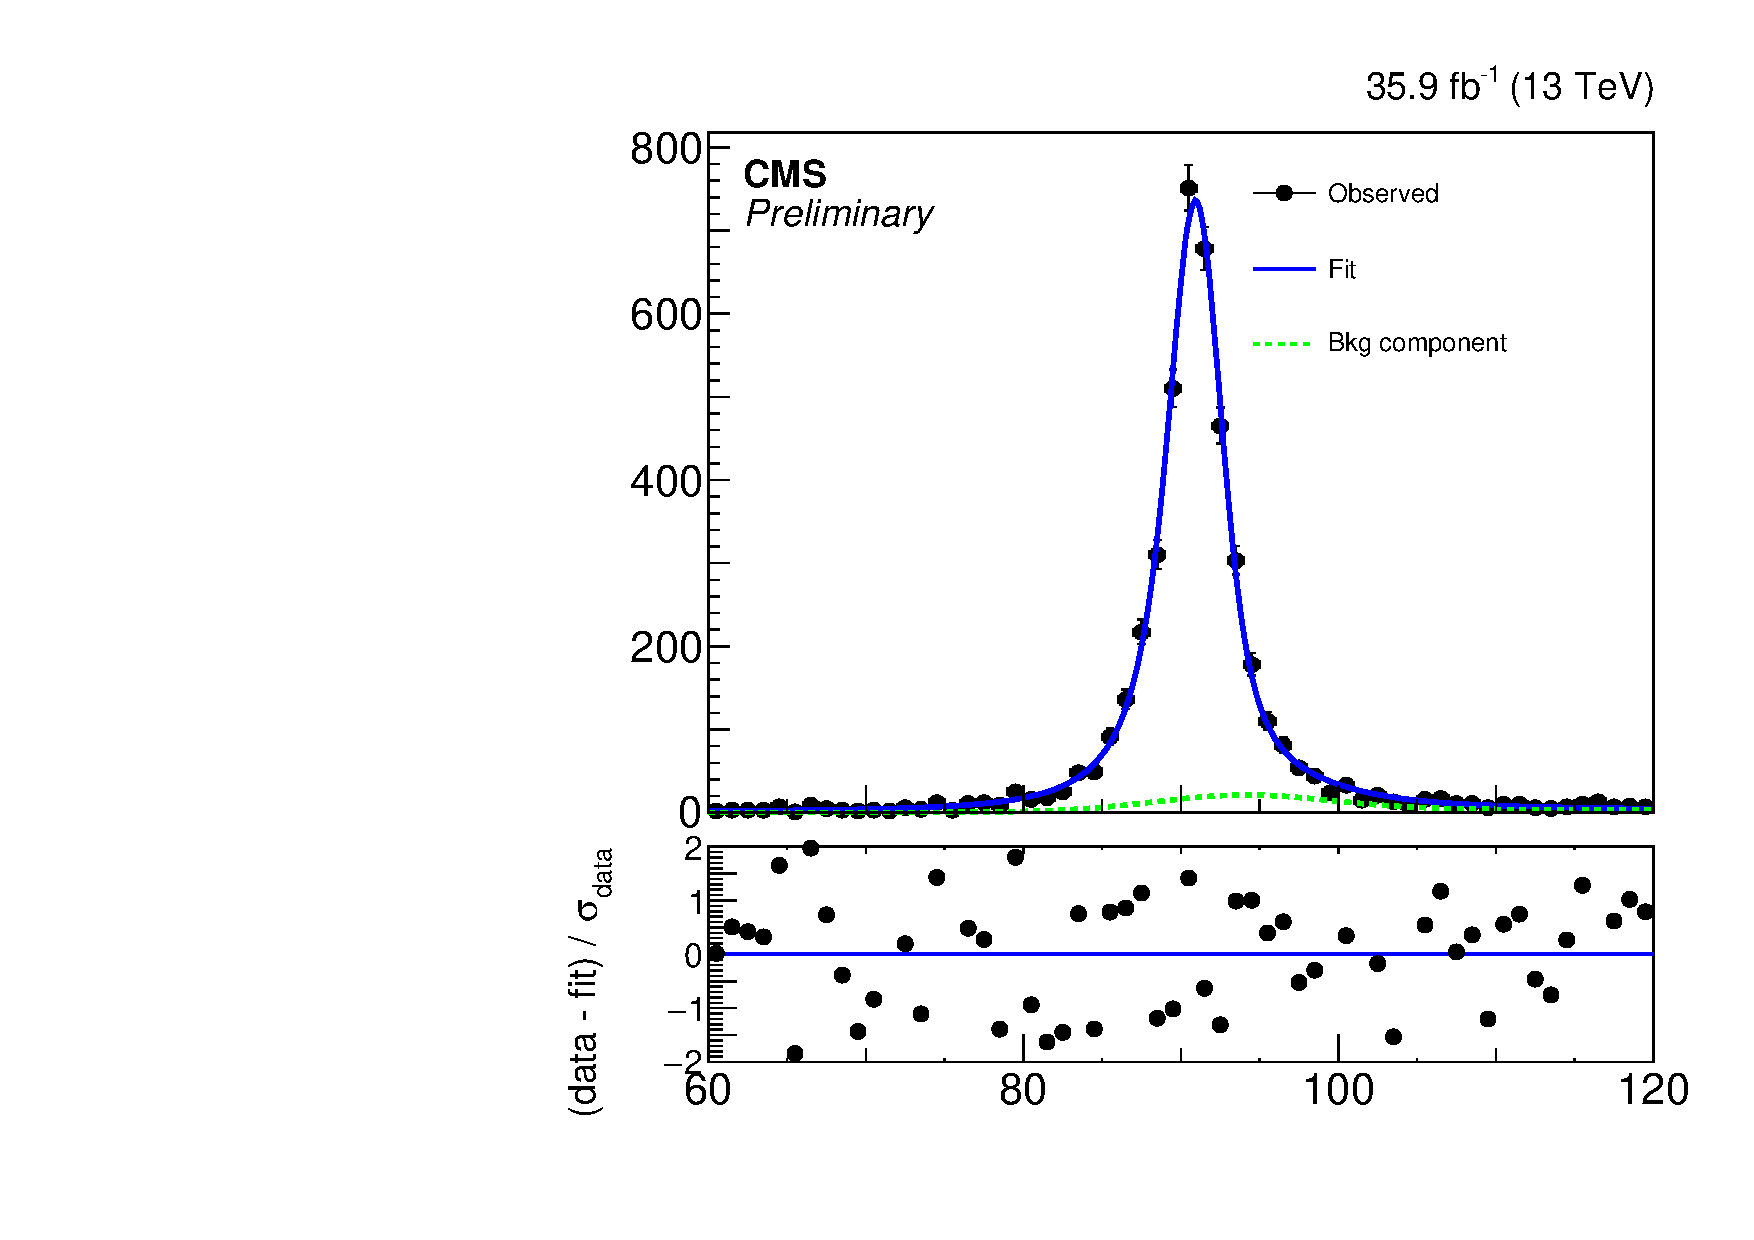
\includegraphics[width=0.47\textwidth]{Analysis/Figures/fit_data_ee_pt_250_6500.pdf}
    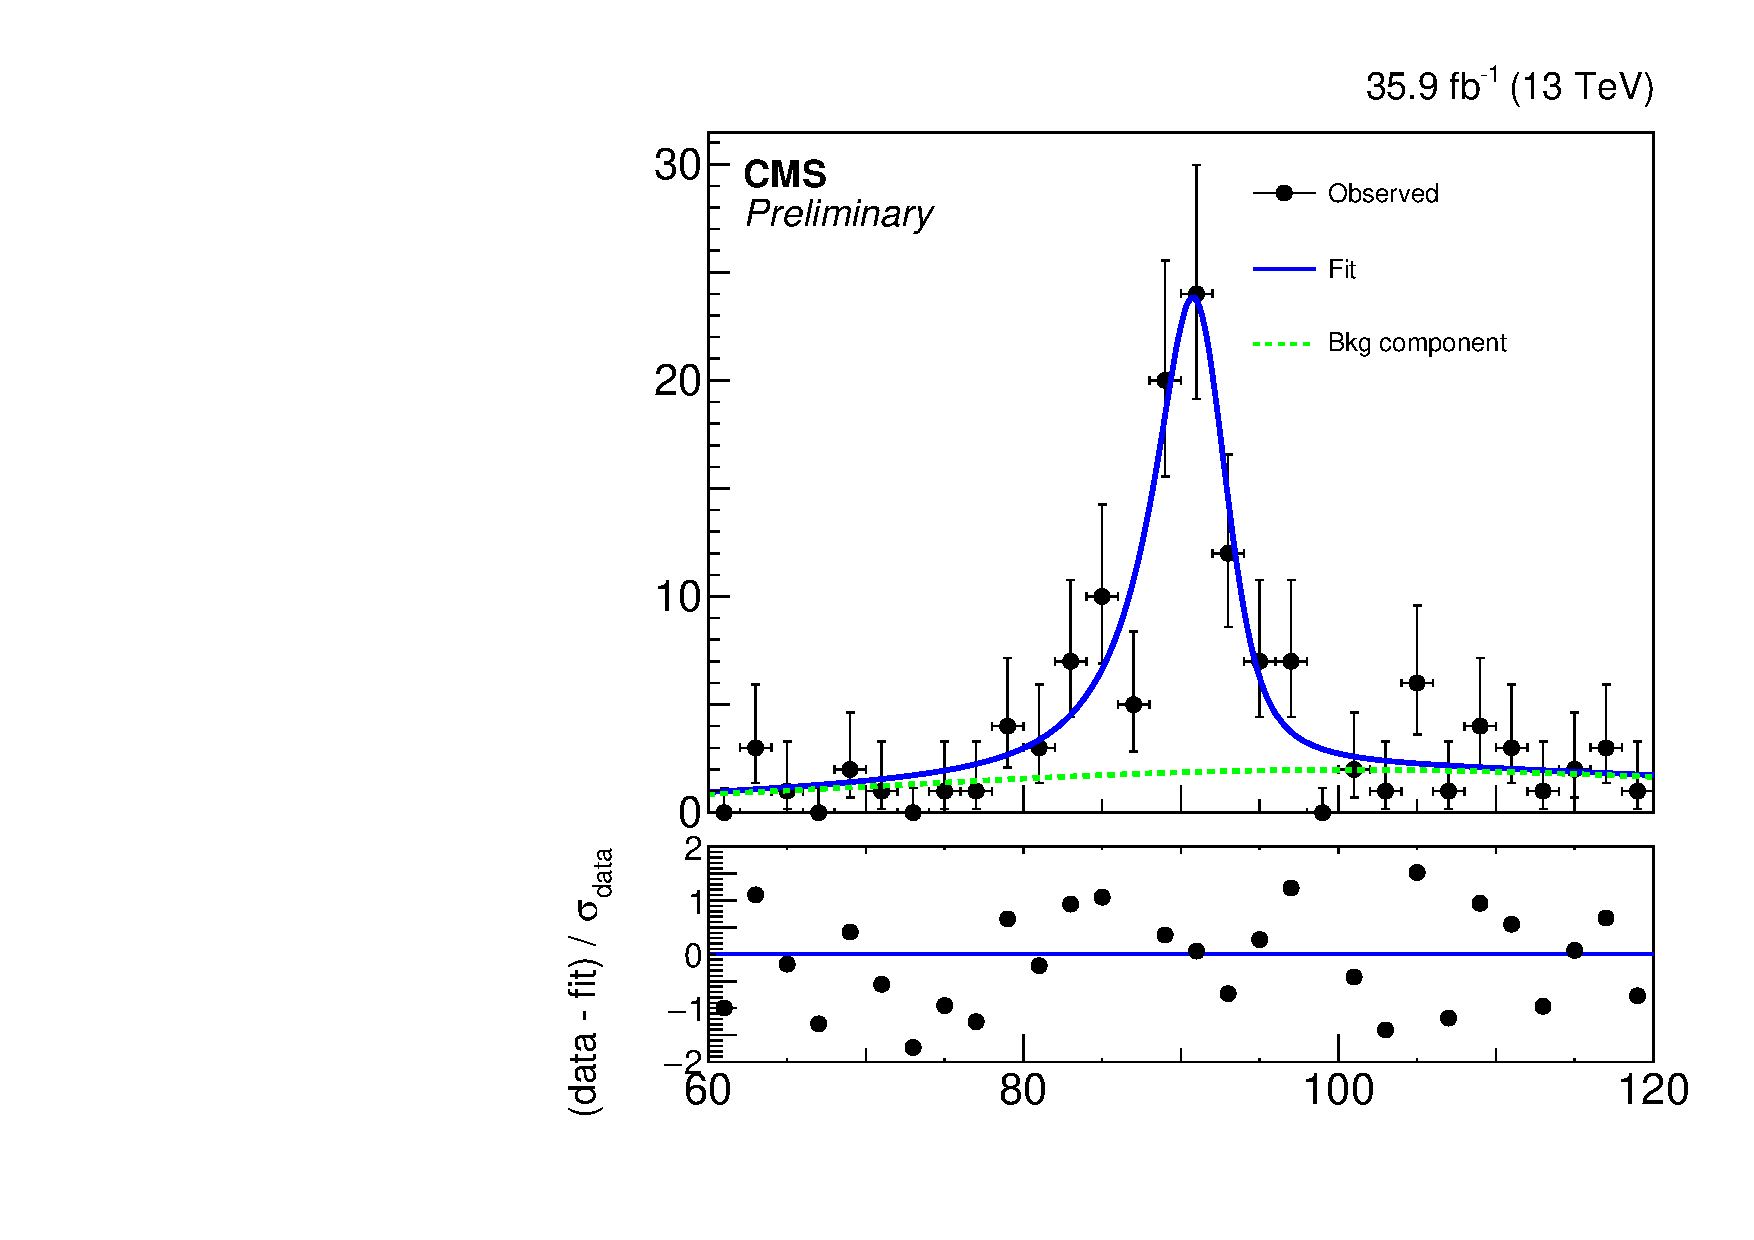
\includegraphics[width=0.47\textwidth]{Analysis/Figures/fit_data_eg_pt_250_6500.pdf}
    \caption{
      Fits to the mass distributions for \Pe\Pe\ (left) and \Pe\Pgg\ (right) selections, in bins of probe $\pt$: $175 < \pt < 200\GeV$ (top), $200 < \pt < 250\GeV$ (middle), $\pt > 250\GeV$ (bottom). 
      The blue solid line represents the full fit model, and the green dashed line its background component.
    }
    \label{fig:efake_fits}
  \end{center}
\end{figure}

The proxy sample for the background estimation is obtained by identical event selection as that described in Sec.~\ref{sec:event_selection}, but with the pixel-seed veto inverted on the photon candidate object.

%%% Systematic uncertainties in this method to estimate the electron misidentification background can be categorized to those related to the TP fit (described in Section~\ref{sec:idsf}) and those related to the applicability of the $R_{\Pe}$ factor.

Figure~\ref{fig:efake_frate} shows the derived $R_{\Pe}$ factor as a function of \ETg. 
The electron proxy sample is reweighted by $R_{\Pe}$ depending on the \pt\ of the electron object.

%%% this file has charged PF veto included, need to swap out
\begin{figure}[htbp]
  \begin{center}
    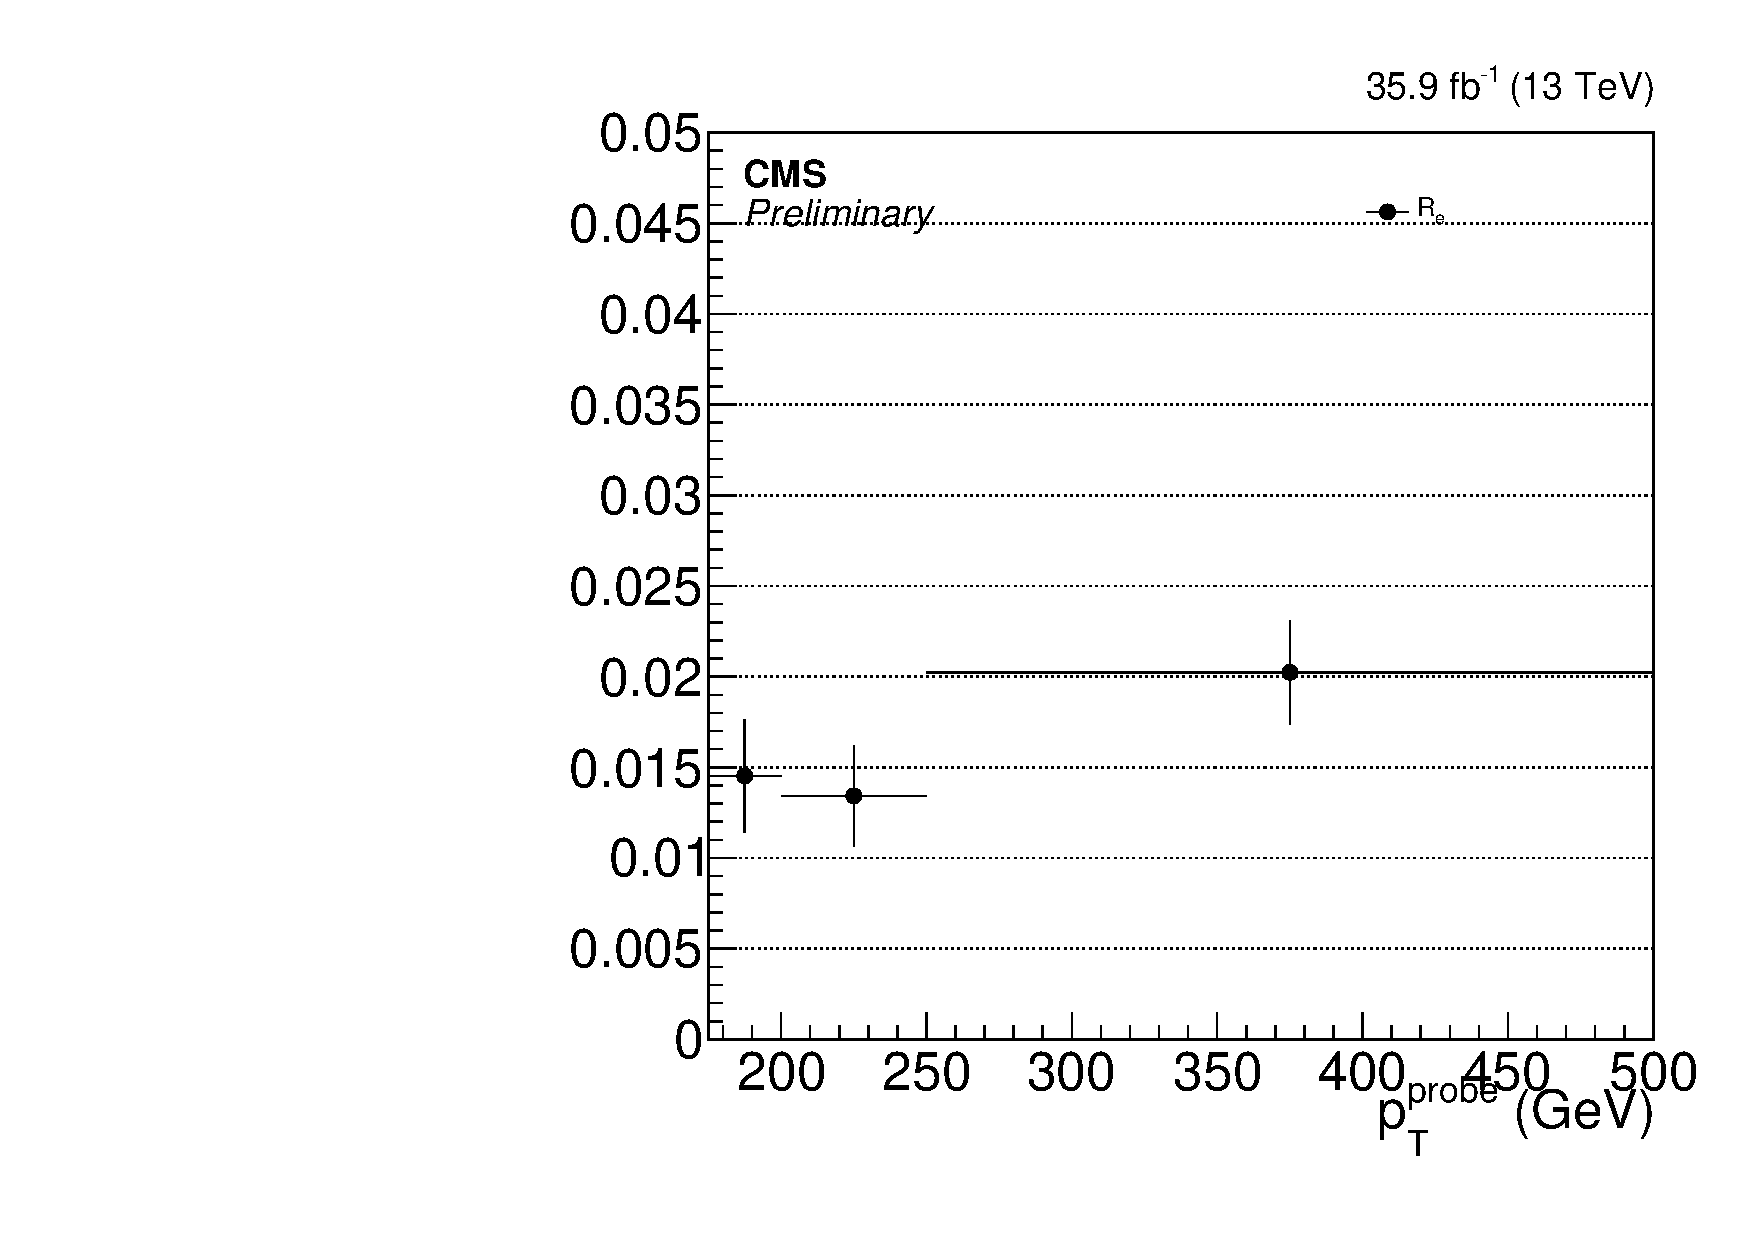
\includegraphics[width=0.49\textwidth]{Analysis/Figures/frate_data_ptalt.pdf} 
    \caption{
      Electron to photon fake rate $R_{\Pe}$.
    }
    \label{fig:efake_frate}
  \end{center}
\end{figure}

\section{Misidentified hadrons}
\label{sec:hfake}

The estimation of hadron misidentification background proceeds in multiple steps. 
First, the fraction of hadronic objects within a pool of photon candidate objects in the photon plus jet control region is measured. 
This measurement is described in detail in Section~\ref{sec:pvsf}.
Figure~\ref{fig:impurity-compsb} and Table~\ref{tab:hfake-impurity-systs} show the final impurity and associated uncertainties as a function of \pt. 

\begin{table}[htbp]
  \centering
  \begin{tabular}{ c|c|c c c c }
    \pt & Nominal & \multicolumn{4}{ |c }{Sources of Systematic Uncertainty} \\
    (GeV) & & Sideband & CH Iso Shape & Signal Shape & Bgkd. Stats \\
    \hline
    (175, 200)  & $4.31 \pm 0.21$ & 0.09 & 0.18 & 0.05 & 0.04 \\
    (200, 250)  & $3.39 \pm 0.17$ & 0.01 & 0.16 & 0.06 & 0.03 \\
    (250, 300)  & $2.44 \pm 0.22$ & 0.14 & 0.16 & 0.06 & 0.05 \\
    (300, 350)  & $1.99 \pm 0.23$ & 0.12 & 0.16 & 0.07 & 0.08 \\
    (350, 400)  & $1.43 \pm 0.28$ & 0.23 & 0.11 & 0.05 & 0.10 \\
    (400, $\infty$)  & $0.63 \pm 0.30$ & 0.27 & 0.09 & 0.05 & 0.05 \\
  \end{tabular}
  \caption{Impurities for photons as a function of \pt.}
  \label{tab:hfake-impurity-systs}
\end{table}

\begin{figure}[htbp]
  \centering
  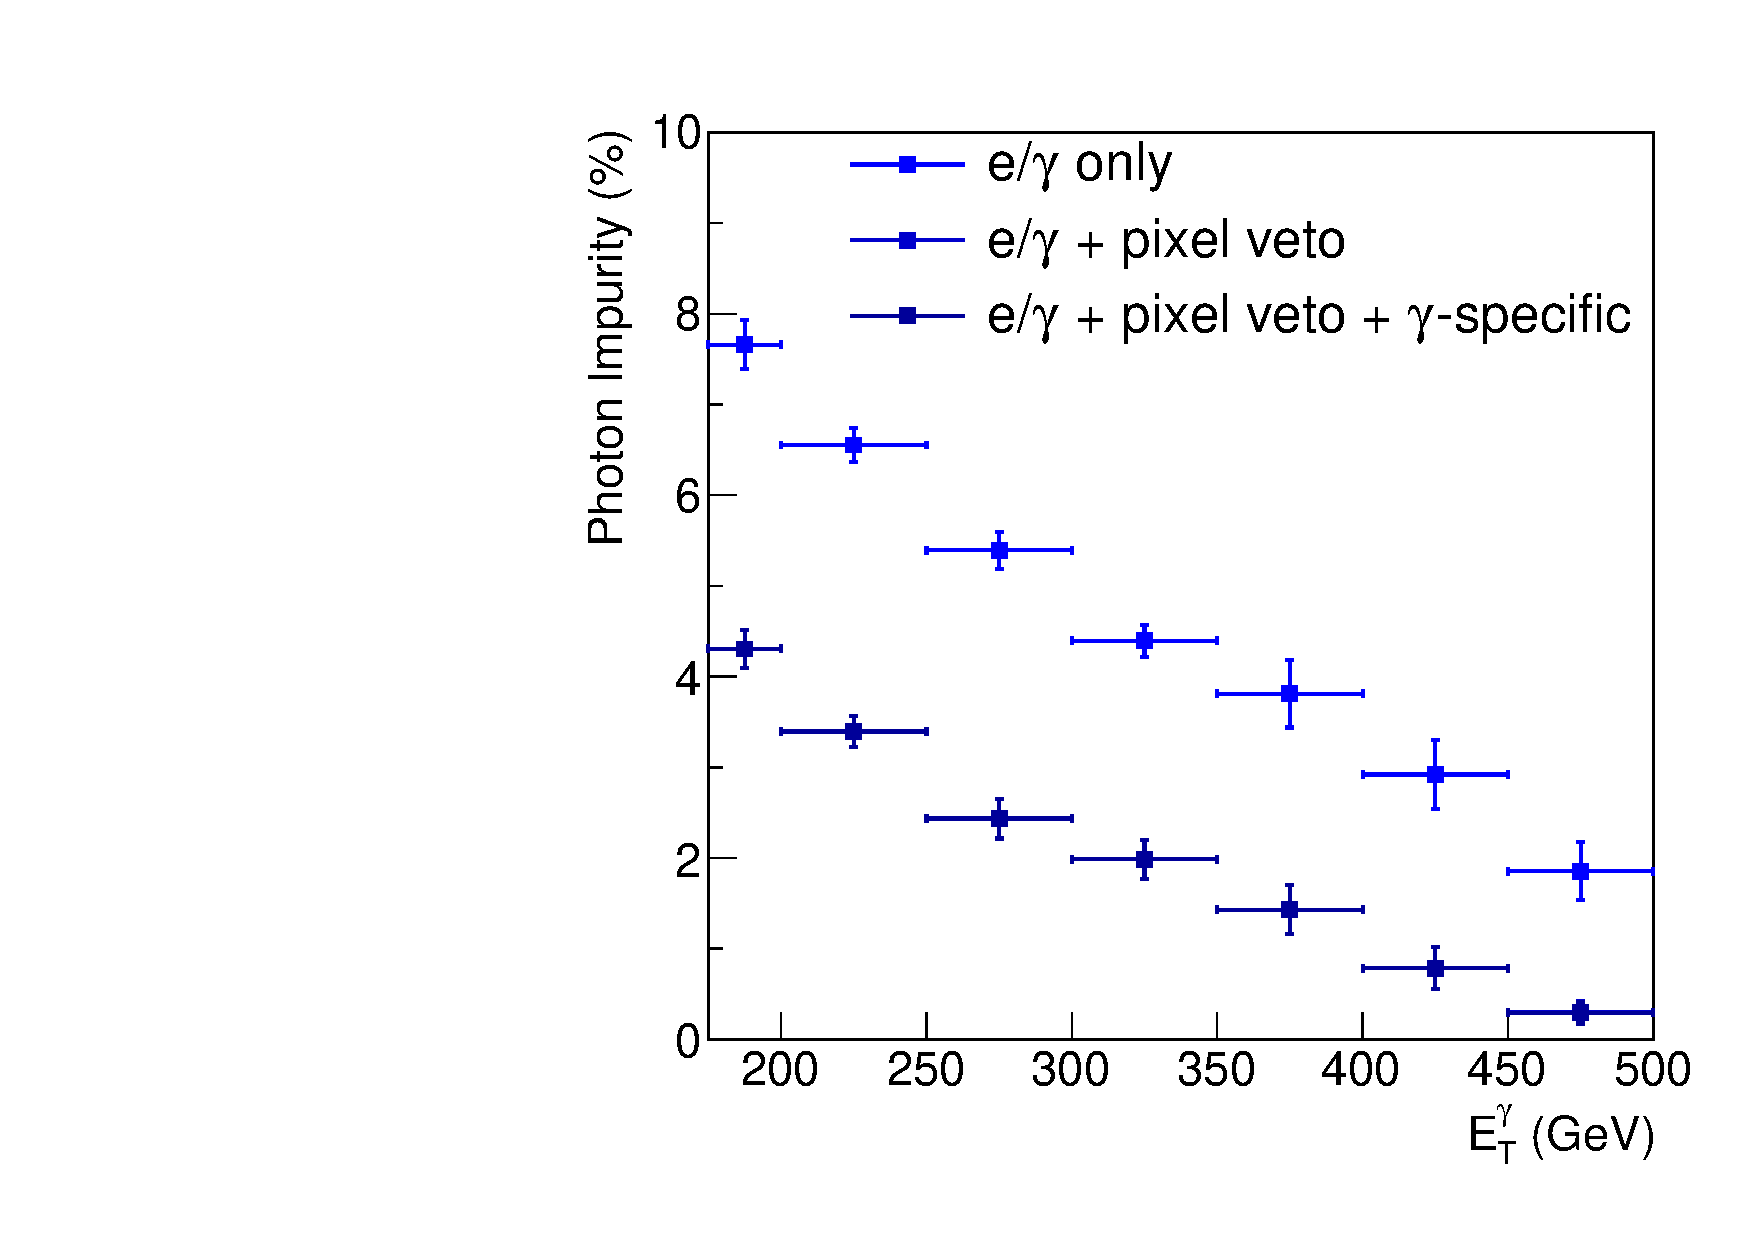
\includegraphics[width=0.49\textwidth]{Analysis/Figures/hfake/plot_impurity_barrel_medium.pdf}
    \caption{
    Impurities for photons as a function of \pt. 
    The different bands show the effects of adding different stages of the full ID, starting with the baseline ID and isolation and successively adding the pixel seed veto.
  }
  \label{fig:impurity-compsb}
\end{figure}

Following this measurement, another control sample is formed where the photon in the photon plus jet sample is replaced by a hadronic proxy object. 
The hadronic proxy object is a reconstructed photon object which pass the photon ID described in Section~\ref{sec:pf_photons} with the execption of failing at least one of the following cuts: 
\begin{itemize}
\item $\sieie < 0.01022$
\item PF Charged Hadron isolation $< 0.441$ GeV .
\end{itemize}
Additionally, we apply a $\met < 60$ GeV cut to make this region orthogonal to the signal region of the analysis.
  
The hadronic transfer factor $R_{h}$, which measures the rate at which hadronic proxy objects result in hadrons that are misidentified as candidate photons, is obtained by dividing the estimated number of misidentified hadrons in the photon plus jet sample by the number of events in the hadron proxy + jet control region as a function of \pt. 
Figure~\ref{fig:hadronTFactor} shows the transfer factor $R_{h}$ along with the various distributions used for its derivation.

\begin{figure}[htbp]
  \begin{center}
    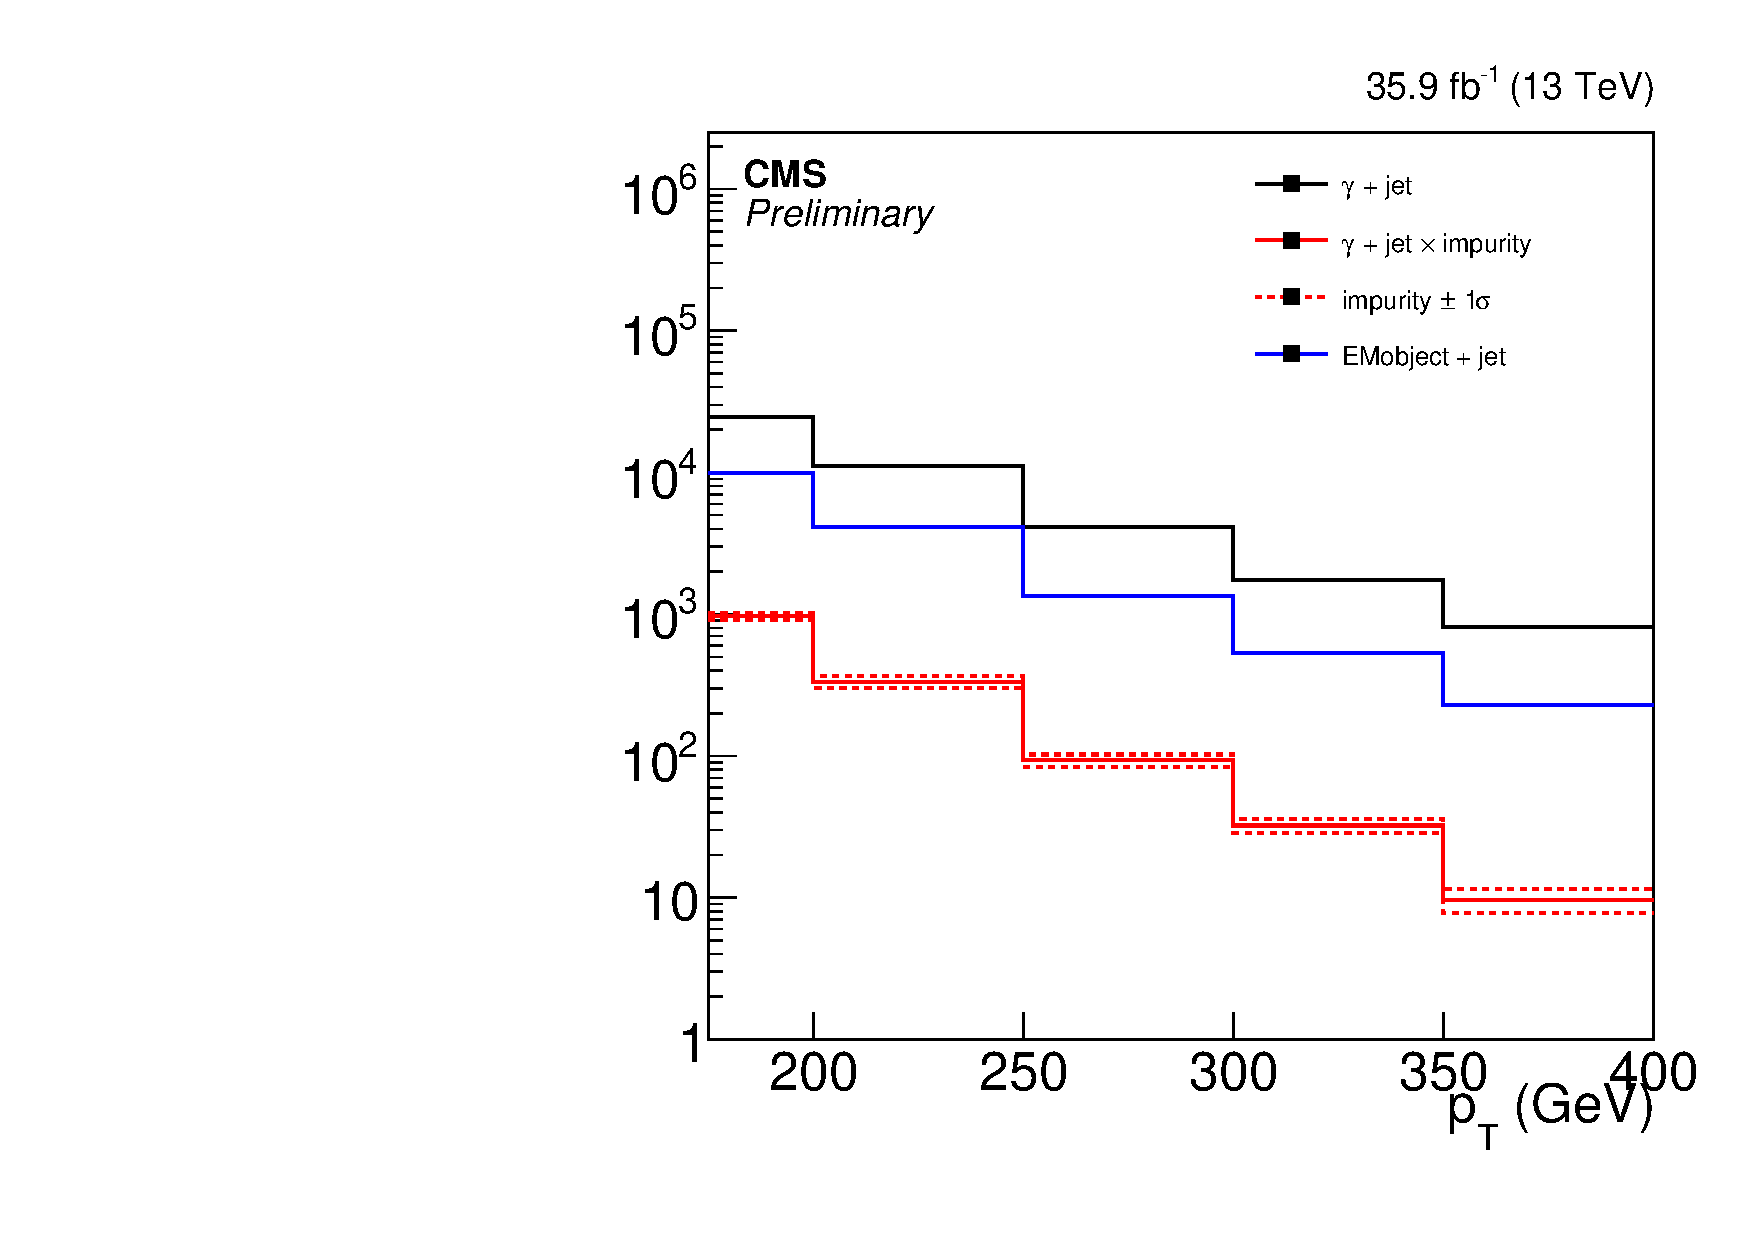
\includegraphics[width=0.45\textwidth]{Analysis/Figures/hfake/distributionsNom.pdf}
    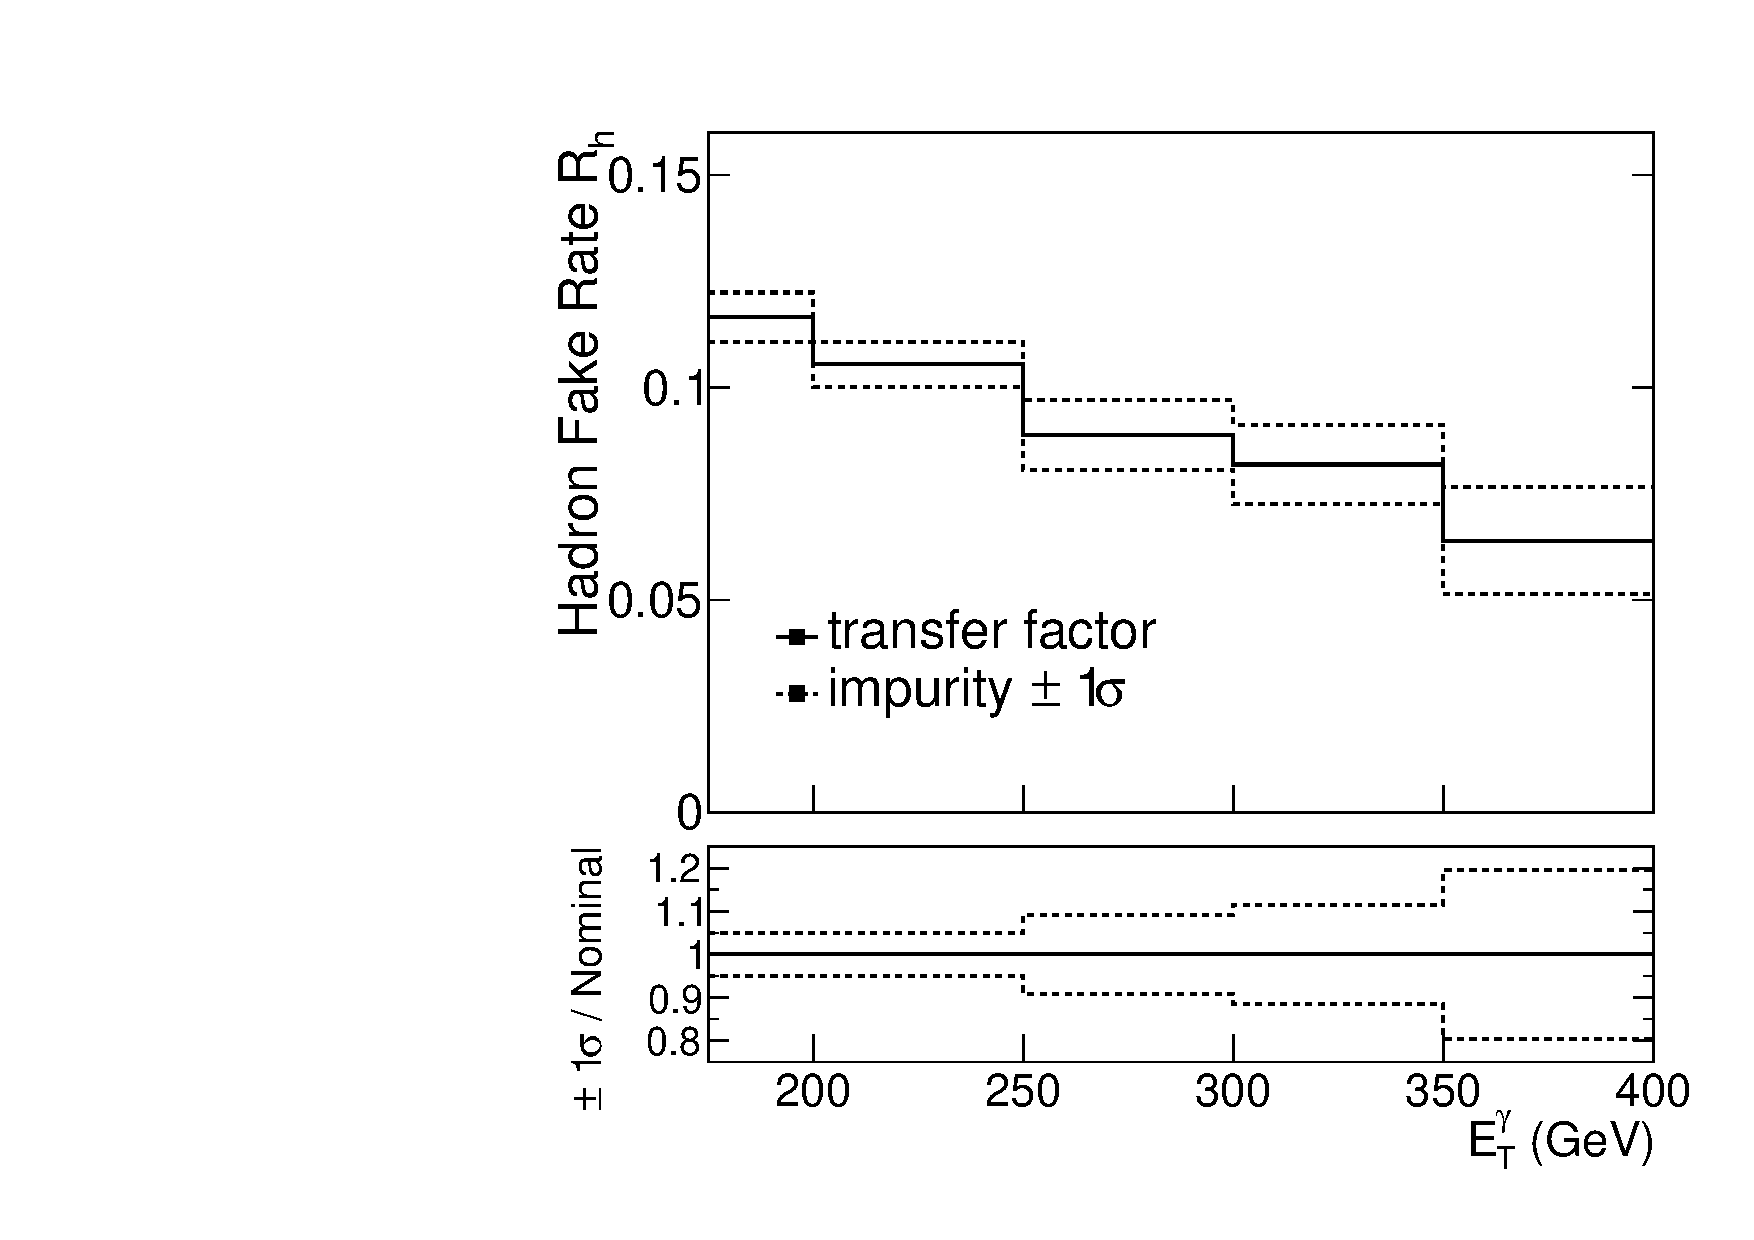
\includegraphics[width=0.45\textwidth]{Analysis/Figures/hfake/tfactorNom.pdf}
    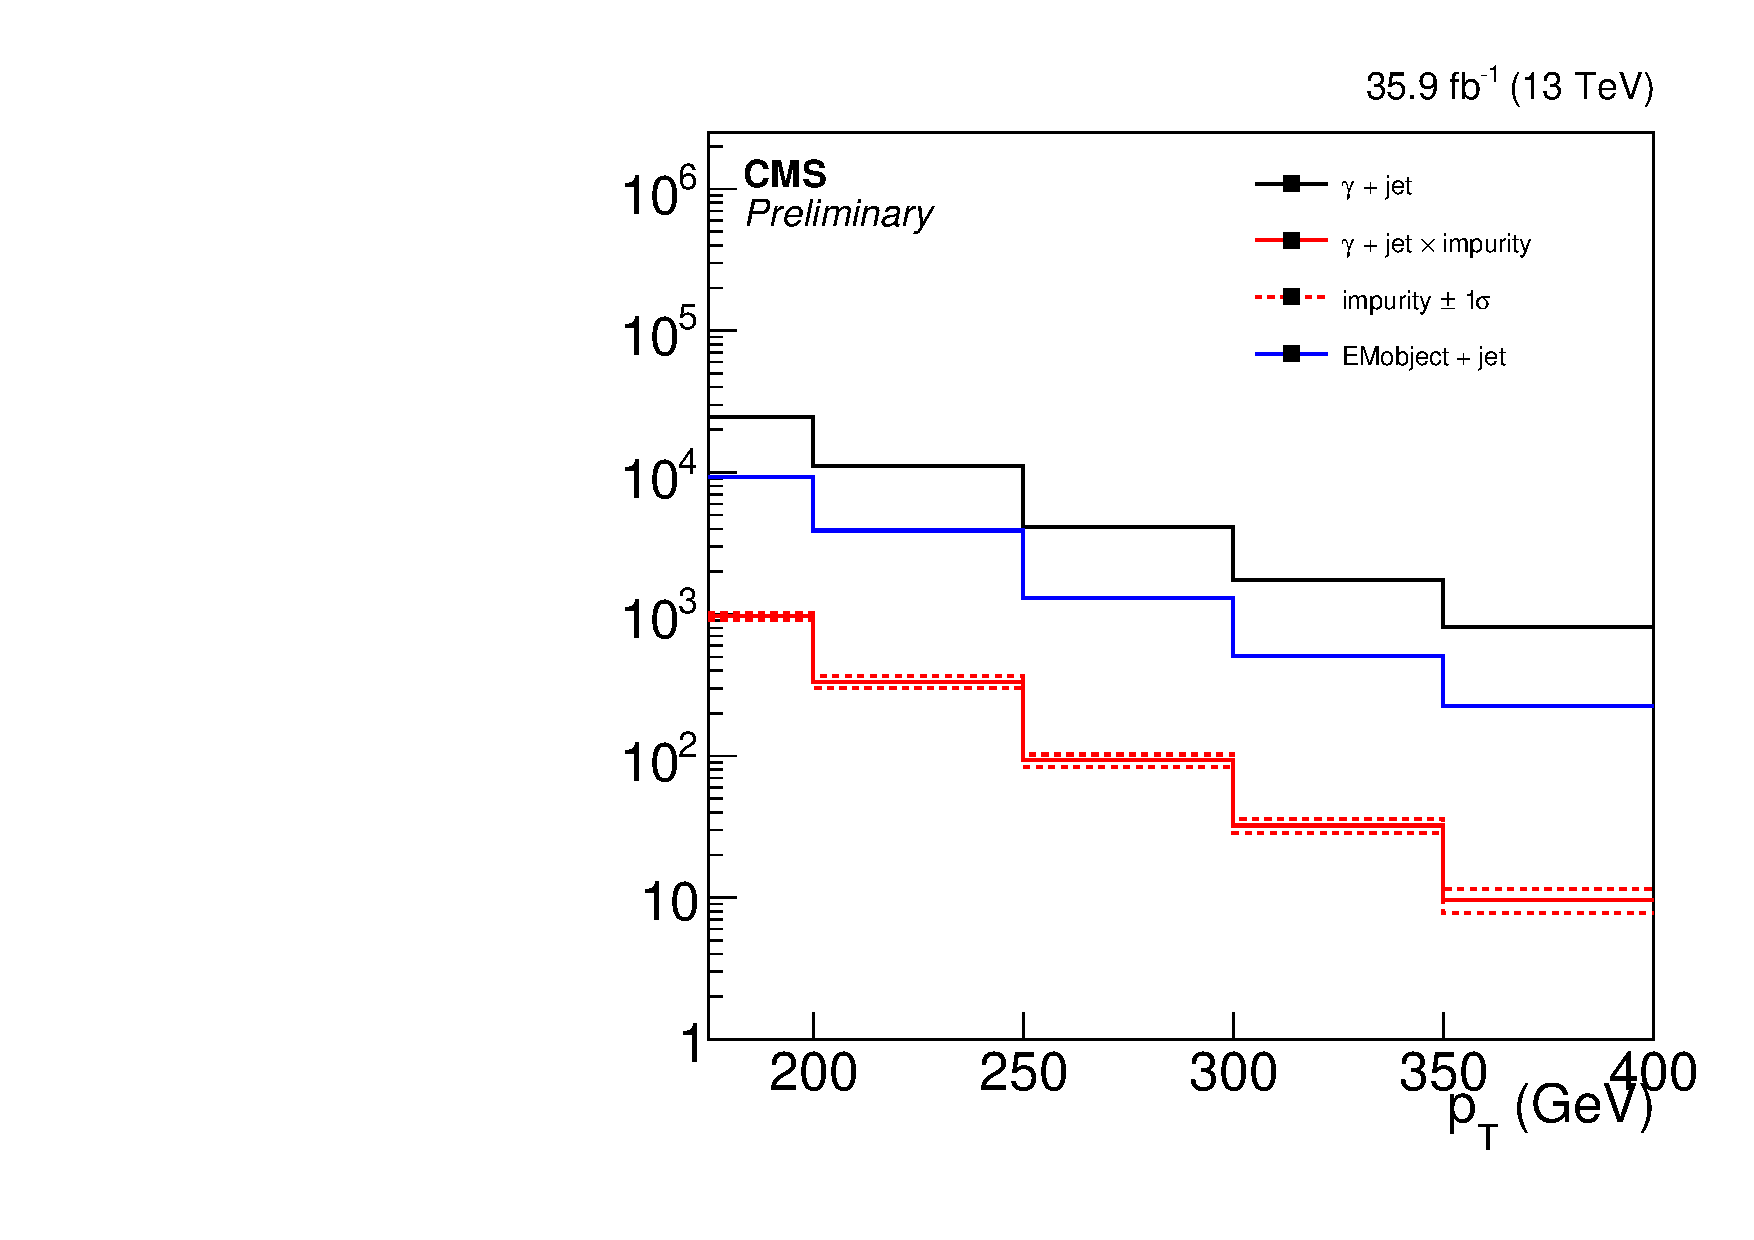
\includegraphics[width=0.45\textwidth]{Analysis/Figures/hfake/distributionsTight.pdf}
    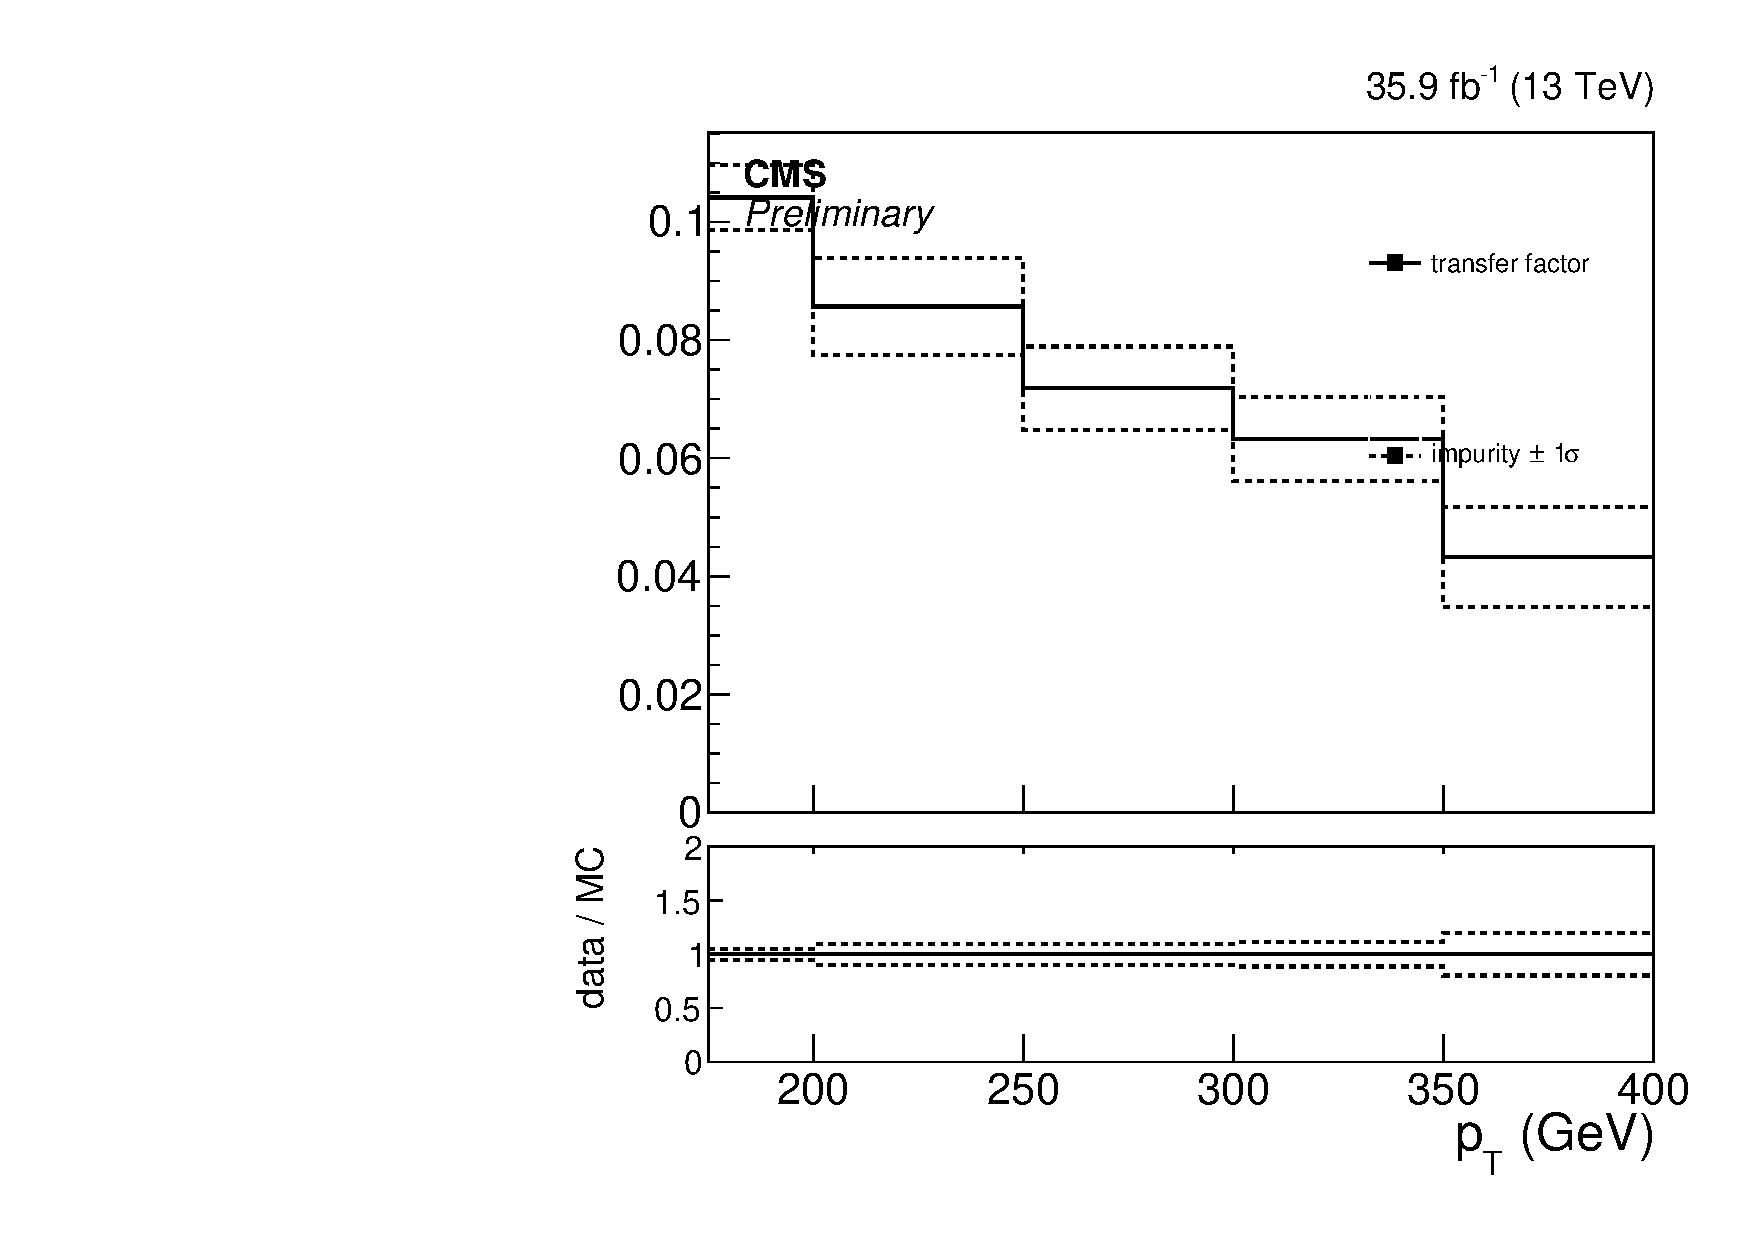
\includegraphics[width=0.45\textwidth]{Analysis/Figures/hfake/tfactorTight.pdf}
    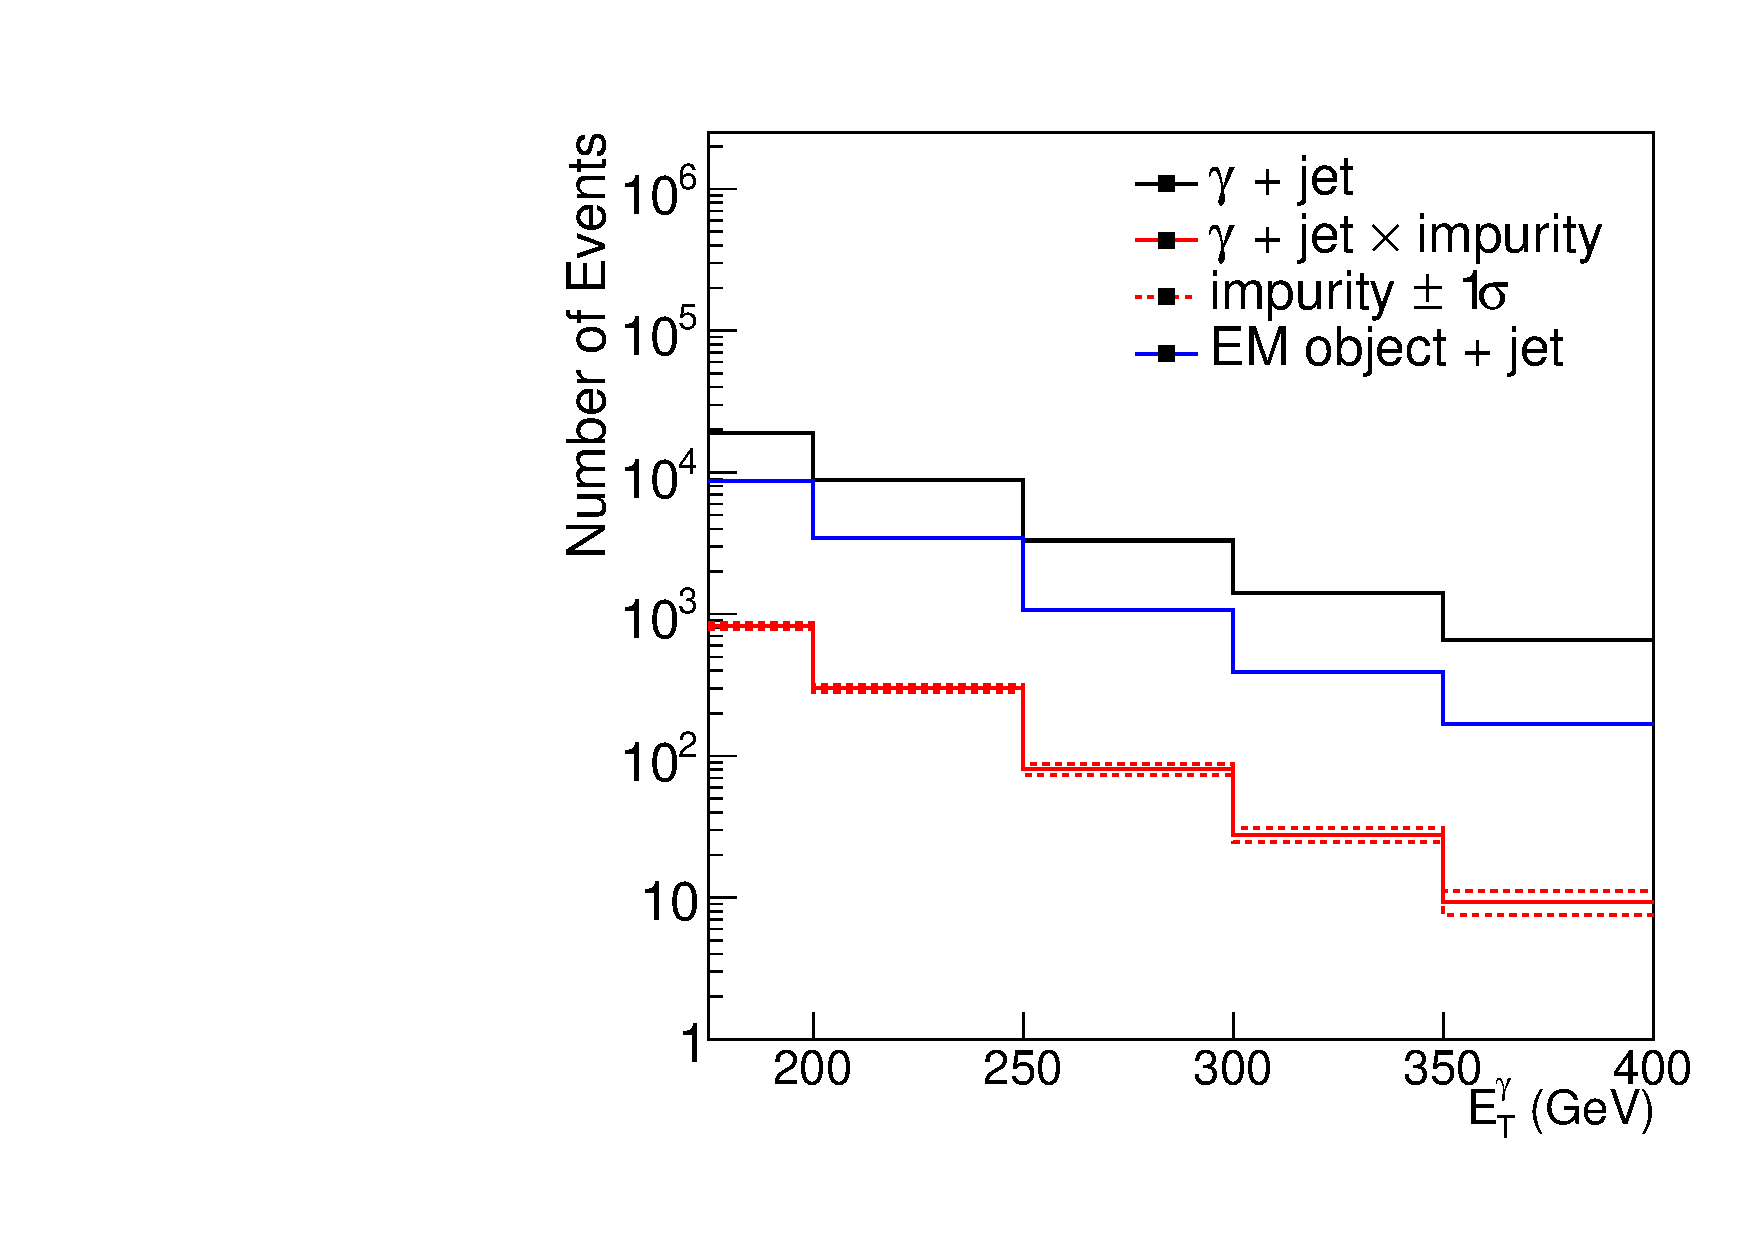
\includegraphics[width=0.45\textwidth]{Analysis/Figures/hfake/distributionsLoose.pdf}
    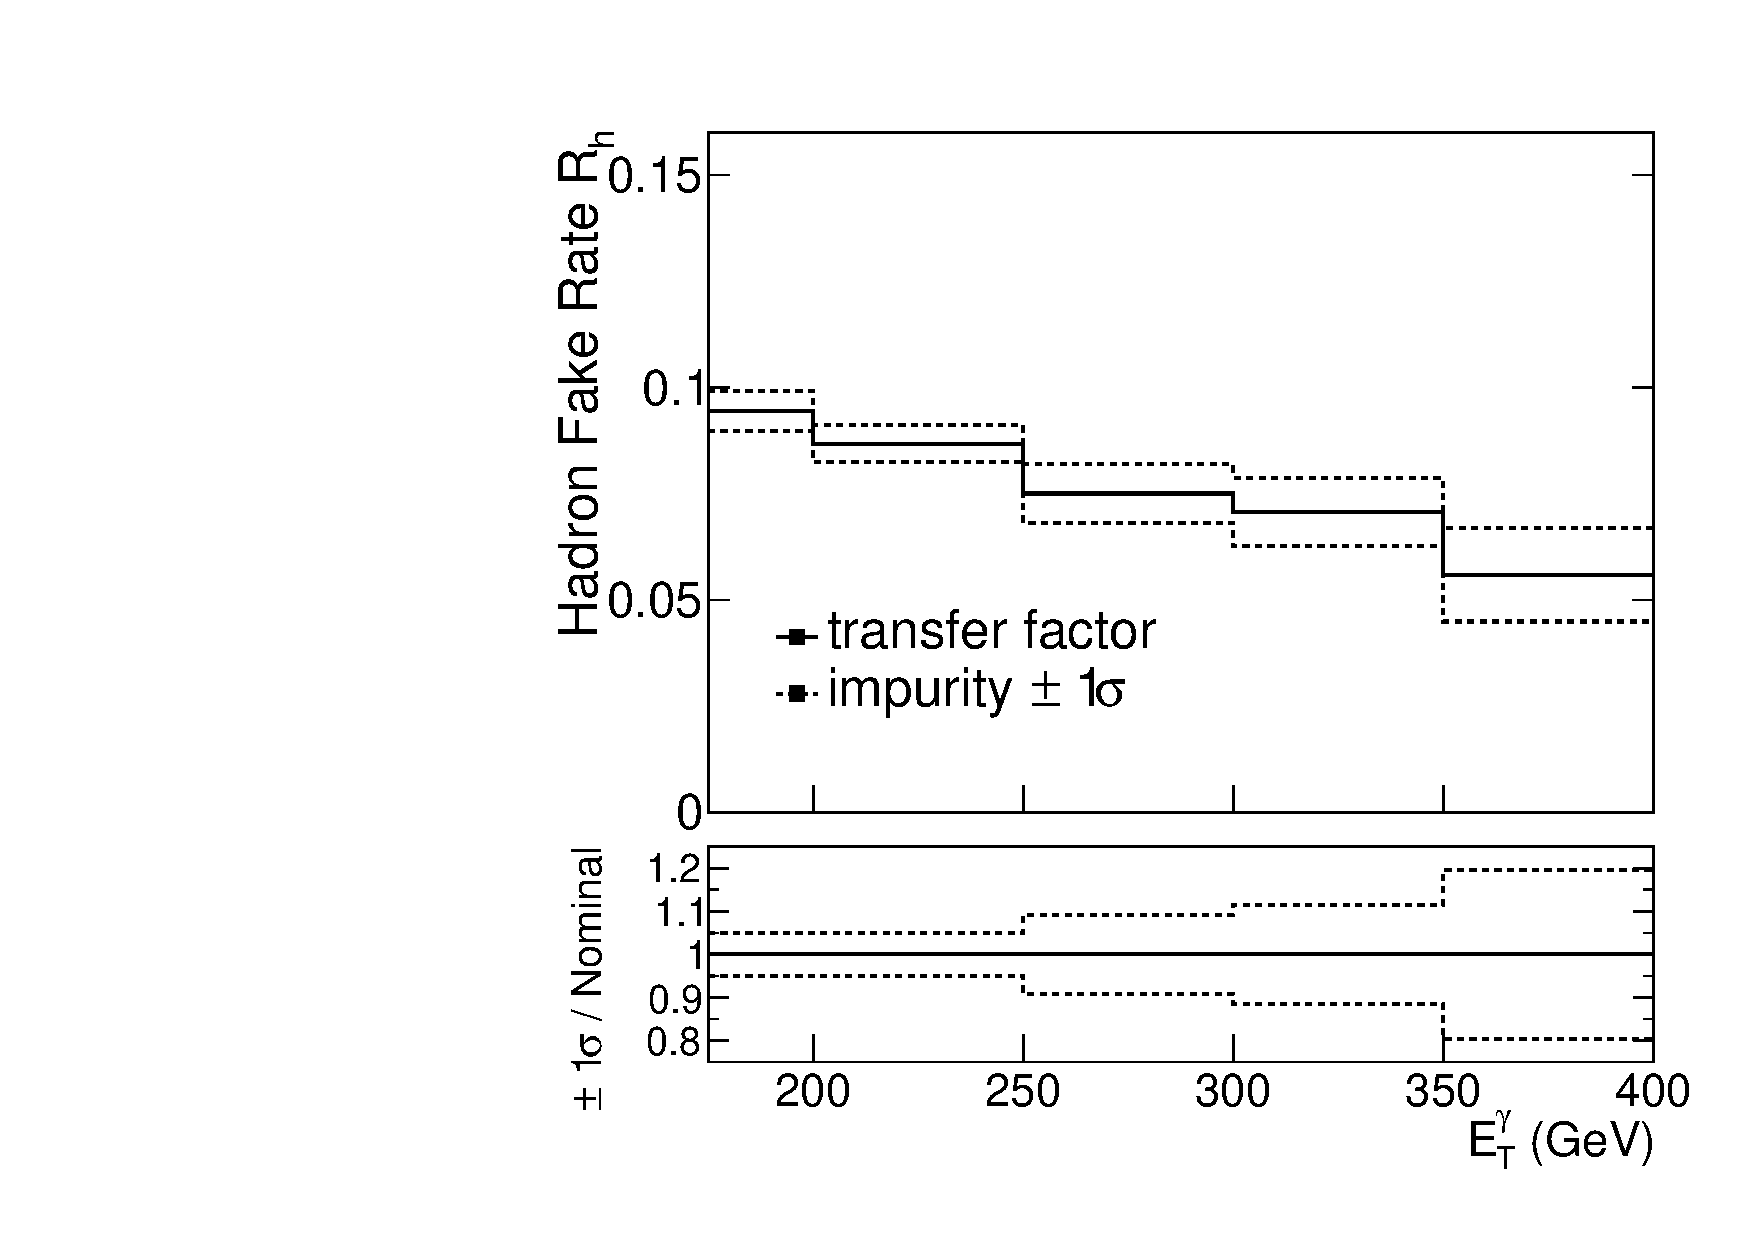
\includegraphics[width=0.45\textwidth]{Analysis/Figures/hfake/tfactorLoose.pdf}
    \caption{
      Left: The \pt\ distribution of the candidate photon object in the photon + jet control sample (black), the result of scaling it with the impurity (red), and the \pt\ distribution of the hadronic proxy object in the proxy + jet control sample (blue).
      Right: Hadronic transfer factor $R_{h}$, which is the ratio of the red and blue distributions in the left plot. 
      Top: Nominal hadron proxy object. 
      Middle: Tighter hadron proxy object. 
      Bottom: Looser hadron proxy object.
    }
    \label{fig:hadronTFactor}
  \end{center}
\end{figure}

Finally, a third control sample of events with a hadronic proxy object and $\met > 170$ GeV is prepared. 
Under the assumption that the $R_{h}$ stays constant regardless of whether the event has a high-\pt\ jet or \met, this proxy plus \met\ sample is then weighted by $R_{h}$ to arrive at an estimate of the misidentified hadron plus \met\ background of this analysis.

%%% need to update these numbers
To estimate the uncertainty on this background, we repeat the above method using tighter and looser definitions of the hadron proxy object.
The tighter definition differs from the nominal by the following cuts:
\begin{itemize}
\item $\rho$-corrected PF Neutral Hadron isolation $< 0.264 + 0.014 \times \pt^\gamma + 0.000019 \times \left( \pt^\gamma \right)^2$. 
\item $\rho$-corrected PF Photon isolation $< 2.362 + 0.0053 \times \pt^\gamma$,
\end{itemize}
and the looser definition differs from the nominal by the following cuts:
\begin{itemize}
\item $\rho$-corrected PF Neutral Hadron isolation $< 10.910 + 0.014 \times \pt^\gamma + 0.000019 \times \left( \pt^\gamma \right)^2$. 
\item $\rho$-corrected PF Photon isolation $< 3.630 + 0.0053 \times \pt^\gamma$.
\end{itemize}

The different distributions from the nominal, tight, and loose selections are shown in Figure~\ref{fig:hadronFakeShapes}. 
The tight and loose shapes are taken as the one sigma band around the nominal estimate. 
Additionally, there is an uncertainty coming from the estimation of the photon purity. 
Figure~\ref{fig:hadronFakePurity} shows the resulting shapes from moving the shapes generated by a one sigma shift in the purity.

\begin{figure}[htbp]
  \begin{center}
    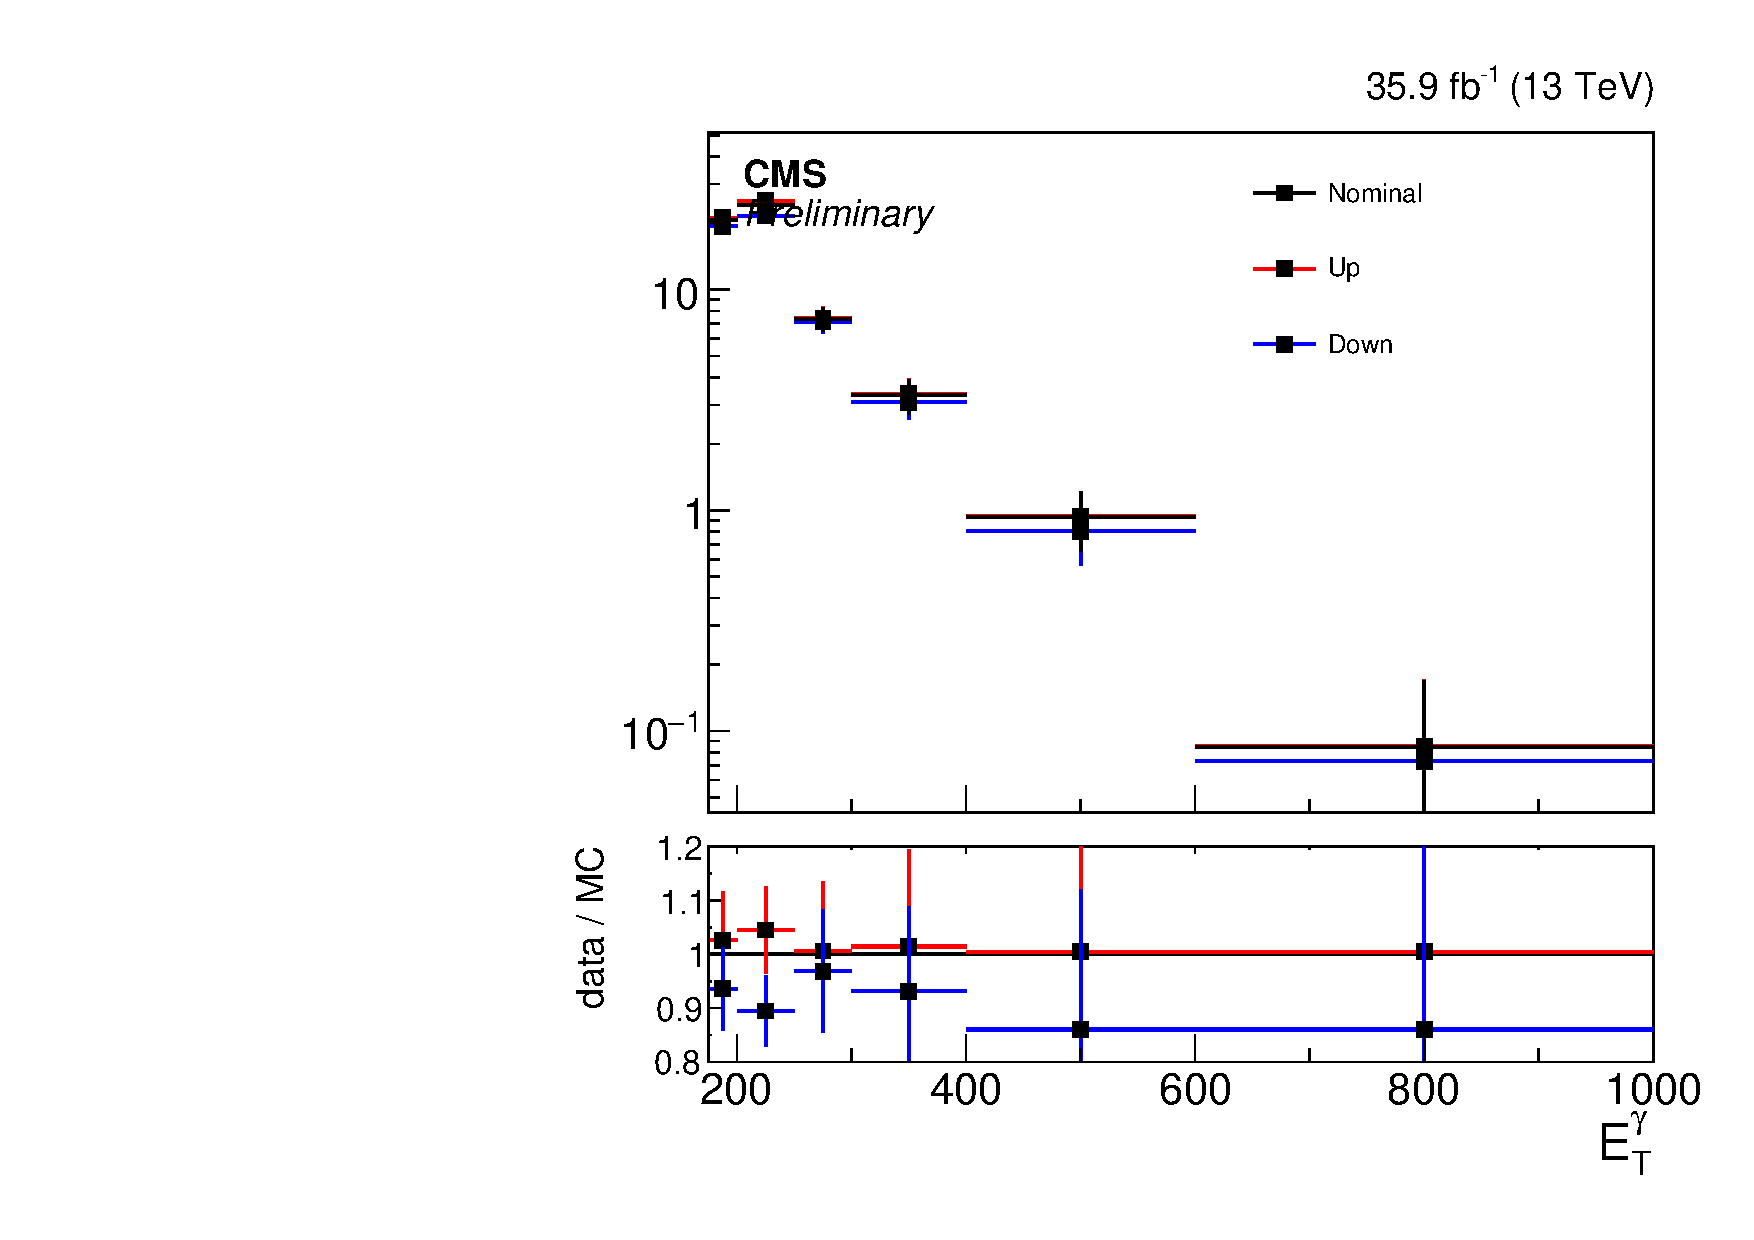
\includegraphics[width=0.49\textwidth]{Analysis/Figures/hfake/shape_sample.pdf}
    \caption{
      The \pt\ distribution of the estimated contribution from hadronic fakes in the signal region. 
      The distribution labeled Up (Down) comes from the tighter (looser) selection. 
      The systematic uncertainty resulting from this variation is around 5\% at the low end of our \pt\ range and increases to 15\% after $\pt > 400$ GeV.
    }
    \label{fig:hadronFakeShapes}
  \end{center}
\end{figure}

\begin{figure}[htbp]
  \begin{center}
    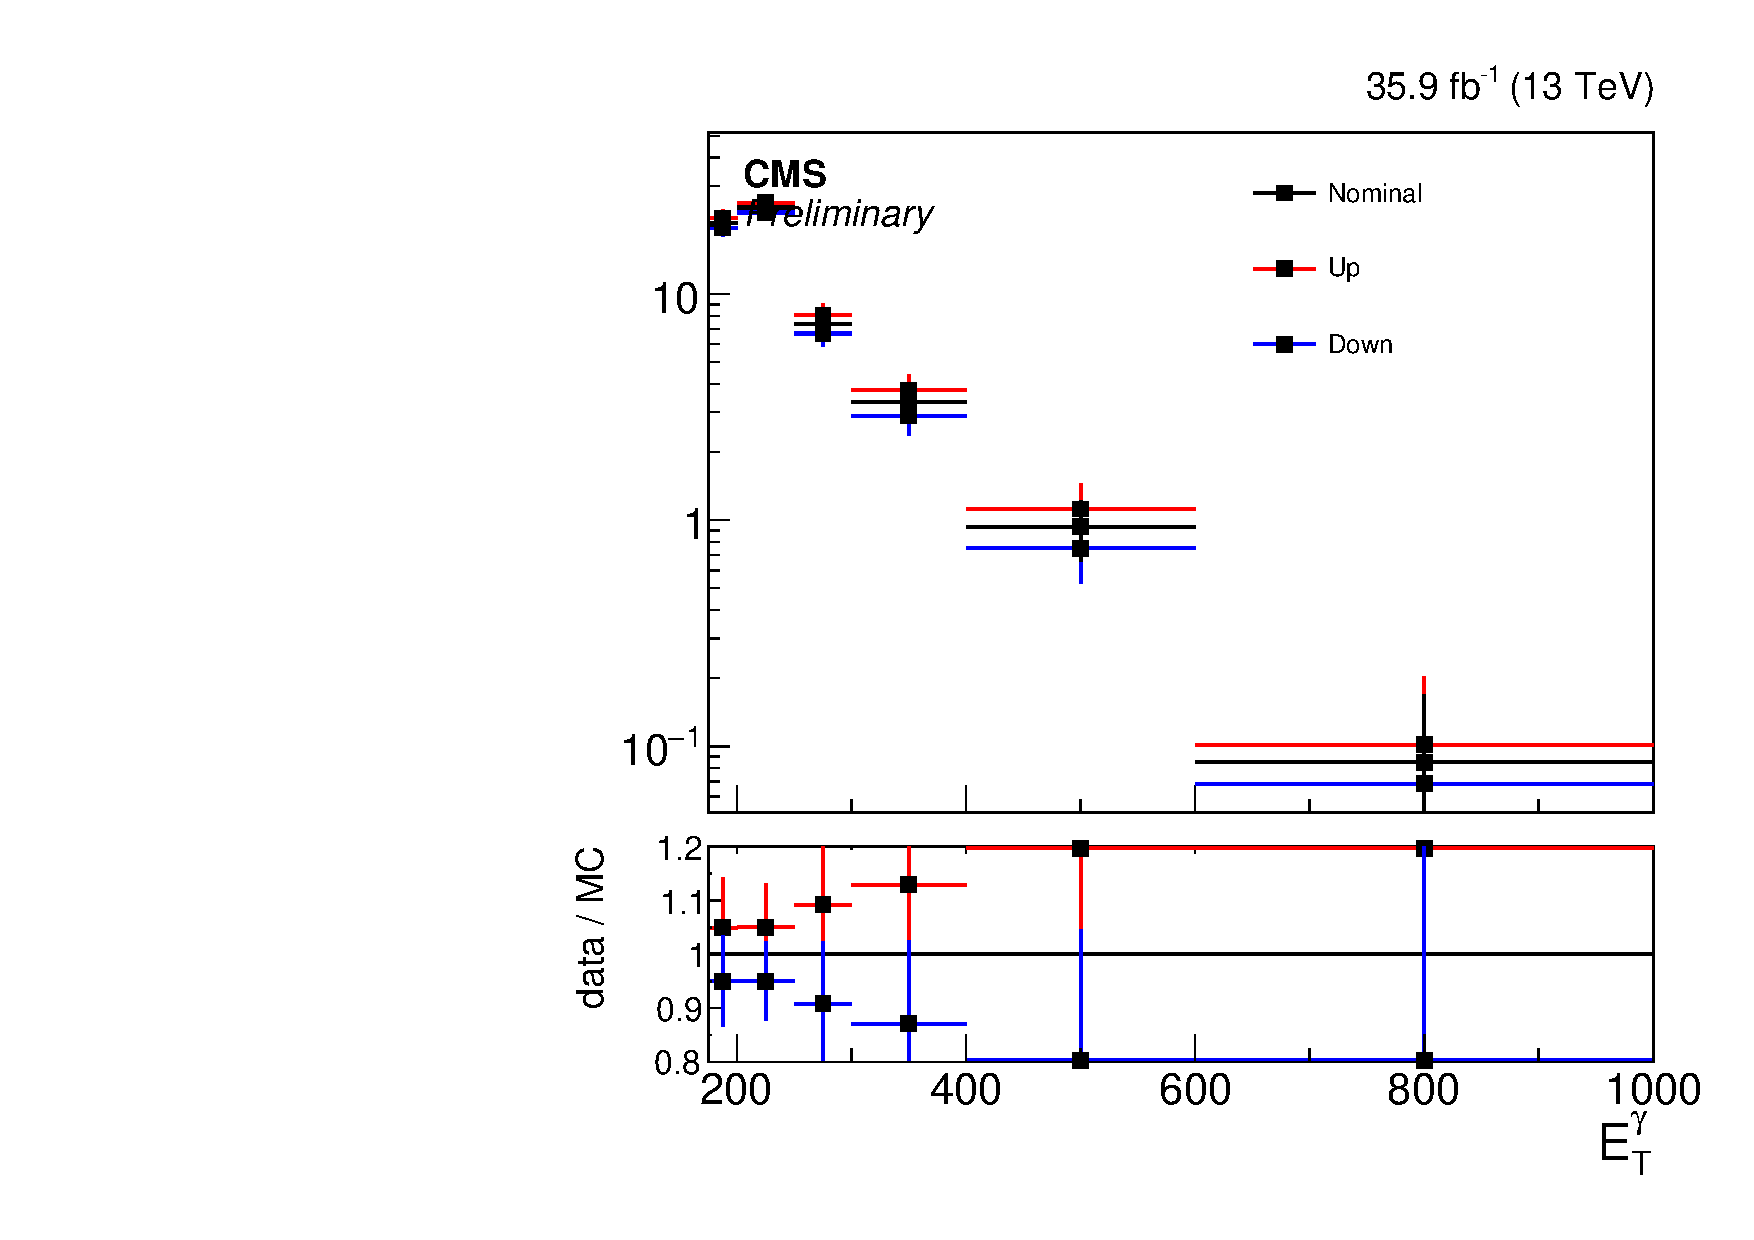
\includegraphics[width=0.49\textwidth]{Analysis/Figures/hfake/shape_purity.pdf}
    \caption{
      The \pt\ distribution of the estimated contribution from hadronic fakes in the signal region. 
      The distribution labeled Up (Down) comes from varying the purity one sigma up (down). 
      The systematic uncertainty resulting from this variation is around 5\% at the low end of the \pt\ range and increases to 20\% after $\pt > 400$ GeV.
    }
    \label{fig:hadronFakePurity}
  \end{center}
\end{figure}

\section{Beam halo}
\label{sec:halo_estimate}

Based on the beam halo features discussed in Section~\ref{sec:halo}, a two-template fit to the $\phi'$ distribution of the photons in the candidate sample, where the templates are that of the halo shower and a uniform distribution, accurately estimates the amount of beam halo background present in the signal region. 
For this analysis, the splitting of the signal region functions in a similar manner, enabling us to determine the beam halo contribution during the signal extraction procedure.

In the horizontal ($H$) and vertical ($V$) signal regions, collision processes occupy the relative fractions of phase space $C_{H} = 1/\pi$ and $C_{V} = (\pi-1)/\pi$, respectively. 
The corresponding fractions for beam halo events are determined by selecting a halo-enriched sample where the halo identification is inverted. 
Thus, a fit of the two signal regions provides an estimate of the overall normalization of the beam halo background, denoted $h$.
 
The \ETg\ dependence of the halo background is encoded in \nhalo[,i], the unit-normalized beam halo prediction in the $i^\mathrm{th}$ bin of the signal region $K \in \{H,V\}$.
Using the notation introduced in Section~\ref{sec:irreducible}, the total estimated background \TK\ in the two signal regions are
\begin{equation}
\begin{aligned}
  \TK[,i] & = C_{K} (\NZg[i] + \NWg[i]) + h \nhalo[,i] + C_{K} b_{K,i} \\
          & = C_{K} (1 + {\fZW[i]}^{-1}) \NZg[i] + h \nhalo[,i] + C_{K} b_{K,i},
\end{aligned}
\end{equation}
where $b_{K,i}$ is the total contribution to bin $i$ of region $K$ from electron and hadron misidentification, ECAL spikes, and other minor SM background processes.

\section{Spikes}
\label{sec:spike_estimate}

Given the observations in Section~\ref{sec:spikes}, the time distribution of spike-like rec hits outside of the window $-15 < t < -10\ns$ (and the equivalent with one-bunch-crossing shift) is understood to be due to delayed interactions of neutral hadrons with the APDs, as documented also in Ref.~\cite{CMS_AN_2010-357}. 
In other words, ECAL spike clusters which survive the time cleaning cut of the standard reconstruction are a part of a broad tail of a distribution, and there is no evidence of spike signals that specifically populate the ``in-time'' region $-3 < t < 3\ns$.

Having established that there is no special population of ECAL spikes in the in-time region, we can estimate the number of ECAL spike events present in the signal candidate sample by an ``ABCD'' method, where
\begin{itemize}
  \item A = Number of clusters with \sieie\ or \sipip\ less than 0.001 and seed time $-15 < t < -10\ns$, counted in the special-reconstruction sample,
  \item B = Number of clusters with both \sieie\ and \sipip\ greather than 0.001 and seed time $-15 < t < -10\ns$, counted in the special-reconstruction sample, 
  \item C = Number of clusters with \sieie\ or \sipip\ less than 0.001 but an in-time seed, counted in the standard-reconstruction sample passing all other signal event selection, 
\end{itemize}
and D is the estimated number of spike events in the signal region, obtained by
\begin{equation}
  D = C \times \frac{B}{A}.
\end{equation}

The special-reconstruction samples for A and B are from the SinglePhoton datasets, with only the timing cleaning removed from the offline reconstruction.
In this way, the selection bias over spikes from the L1T, HLT, and offline reconstruction is equally applied to samples A, B, and C.

Plugging in the observed numbers, we have
\begin{align*}
  A & = 4969 \\
  B & = 1180 \\
  C & = 54 \\
  \therefore D & = 12.8 \pm 1.8 \text{(stat.)}
\end{align*}

There are, however, at least two reasons to believe that this method overestimates the number of spike events in the signal region. 
One is that the population C contains some physical, prompt photon clusters that just happens to be narrow, as observed in Fig.~\ref{fig:sieie_mc}. 
Another reason is that there is likely a correlation between the cluster width and the seed time such that the ratio of true D to C is smaller than $B/A$.
This statement is based on the standard hypothesis that the wide-cluster spike is an ECAL spike embedded in a physical EM shower cluster. 
Under this model, spikes in wide clusters are mainly caused by prompt neutral hadrons in a jet, which implies that they strongly prefer seed time $-15 < t < -10\ns$. 
Given that this is a minor background with a relatively large uncertainty, as described below, we will still use this estimate as the nominal value of predicted spike contribution in the signal region.

The uncertainty in the estimate of D is evaluated by two modifications to A, B, and C.
First, the three values are recomputed with using $\sieie < 0.001$ as the only definition of narrow cluster. 
This results in a minor change of the value of D of $12.1 \pm 1.7$. Next, A and B are computed using a lower-\pt SinglePhoton sample, requiring triggers Photon135\_PFMET100 or Photon120\_R9Id90\_HE10\_IsoM to have fired, instead of the signal trigger. 
The second modification gives $D=9.1 \pm 1.3$. 
We then take twice the discrepancy between the nominal D and the D value from the second modification as the systematic uncertainty in the spike background estimate.

\section{Minor SM Backgrounds}
\label{sec:minorsm}

After the full selection described in Section~\ref{sec:event_selection}, the SM \gj, \ttg, VV\Pgg, \zllg, and $\PW\to\ell\Pgn$ processes are minor ($\sim$10\%) background processes in the signal region. 
These processes, collectively denoted as minor SM backgrounds, contribute in the signal region when the jet energy is severely mismeasured or the leptons fail to be reconstructed resulting in large \met in the signal region. 
However, the \met is typically aligned with the photon or one of the jets in such cases, and therefore various selections on the kinematic relations between the \met, photons, and jets are used to reduce these backgrounds to a manageable rate. 
The estimates for all five processes are taken from \MGvATNLO~\cite{} simulations at LO in QCD and are listed in Tables~\ref{tab:yield_mask_horizontal} and~\ref{tab:yield_mask_vertical}.

\section{Statistical Interpretation}
\label{sec:interpretation}

The potential signal contribution is extracted from the data via simultaneous fits to the
\ETg\ distributions in the signal and control regions defined in Section~\ref{sec:event_selection}. 
Uncertainties in various quantities are represented by nuisance parameters in the fit. 
Predictions for \zinvg, \wlng, and the beam halo backgrounds are varied in the fit. 
Beam halo is not a major background, but the extraction of its rate requires a fit to the observed distributions in the signal region.

Free parameters of the fit are the yield of \zinvg\ background in each bin of the signal regions (\NZg[i]) and the overall normalization of the beam halo background ($h$). 
Bin-by-bin yields of \wlng\ and \zllg\ samples in all regions are related to the yield of \zinvg\ through the MC prediction through the transfer factors defined in Section~\ref{sec:irreducible}. 
The transfer factors are allowed to shift within the aforementioned theoretical and experimental uncertainties.

The background-only likelihood that is maximized in the fit is
\begin{equation}
\begin{aligned}
  \mathcal{L} & = \prod_{i} \left\{ \mathcal{L_{\text{signal}}} \times \mathcal{L_{\text{single-lepton}}} \times \mathcal{L_{\text{dilepton}}} \right\} \times \mathcal{L_{\text{nuisances}}} \\
  & = \prod_{i} \left\{
    \prod_{K=H,V} \mathcal{P}\left( d_{K, i} \left| \TK[,i] (\vec{\theta} \right.) \right) \times \prod_{\ell=\Pe,\Pgm} \mathcal{P}\left( d_{\ell\Pgg, i} \left| \Tl[,i] (\vec{\theta}) \right. \right)
    \times \prod_{\ell=\Pe,\Pgm} \mathcal{P}\left( d_{\ell\ell\Pgg, i} \left| \Tll[,i] (\vec{\theta}) \right. \right)
    \right\}  \times \prod_{j} \mathcal{N}(\theta_j) \\
  & = \prod_{i} \left\{
  \begin{gathered}
    \prod\limits_{K=H,V} \mathcal{P}\biggl( d_{K, i} \biggl| \left(1 + {\fZW[,i]}^{-1}(\vec{\theta})\right) C_{K} \NZg[i] + h \nhalo[,i](\vec{\theta}) + C_{K} b_{K, i}(\vec{\theta}) \biggr. \biggr) \\
    \times \prod\limits_{\ell=\Pe,\Pgm} \mathcal{P}\biggl( d_{\ell\Pgg, i} \biggl| \frac{\NZg[i]}{\RWl[,i](\vec{\theta}) \fZW[,i] (\vec{\theta})} + b_{\ell\Pgg, i}(\vec{\theta}) \biggr. \biggr) \\
    \times \prod\limits_{\ell=\Pe,\Pgm} \mathcal{P}\biggl( d_{\ell\ell\Pgg, i} \biggl| \frac{\NZg[i]}{\RZll[,i](\vec{\theta})} + b_{\ell\ell\Pgg, i}(\vec{\theta}) \biggr. \biggr)
  \end{gathered} \right\}
  \times \prod_{j} \mathcal{N}(\theta_j),
\end{aligned}
\end{equation}
following the notation introduced in Section~\ref{sec:irreducible}, and where $\mathcal{P}
(n\vert\lambda)$ is the Poisson probability of $n$ for mean $\lambda$, $\mathcal{N}$ denotes the unit normal distribution, and $d_{X,i}$ is the observed number of events in bin i of region X.
Systematic uncertainties are treated as nuisance parameters in the fit and are represented by
$\vec{\theta}$.
Each quantity $Q_{j}$ with a nominal value $\overline{Q}_{j}$ and a standard deviation of the systematic uncertainty $\sigma_{j}$ appears in the likelihood function as $\overline{Q}_{j}\exp(\sigma_{j}\theta_{j})$.

\section{Results}
\label{sec:results}

\subsection{Pre-fit and post-fit distributions}
\label{sec:distributions}

\begin{figure}[htbp]
  \centering
    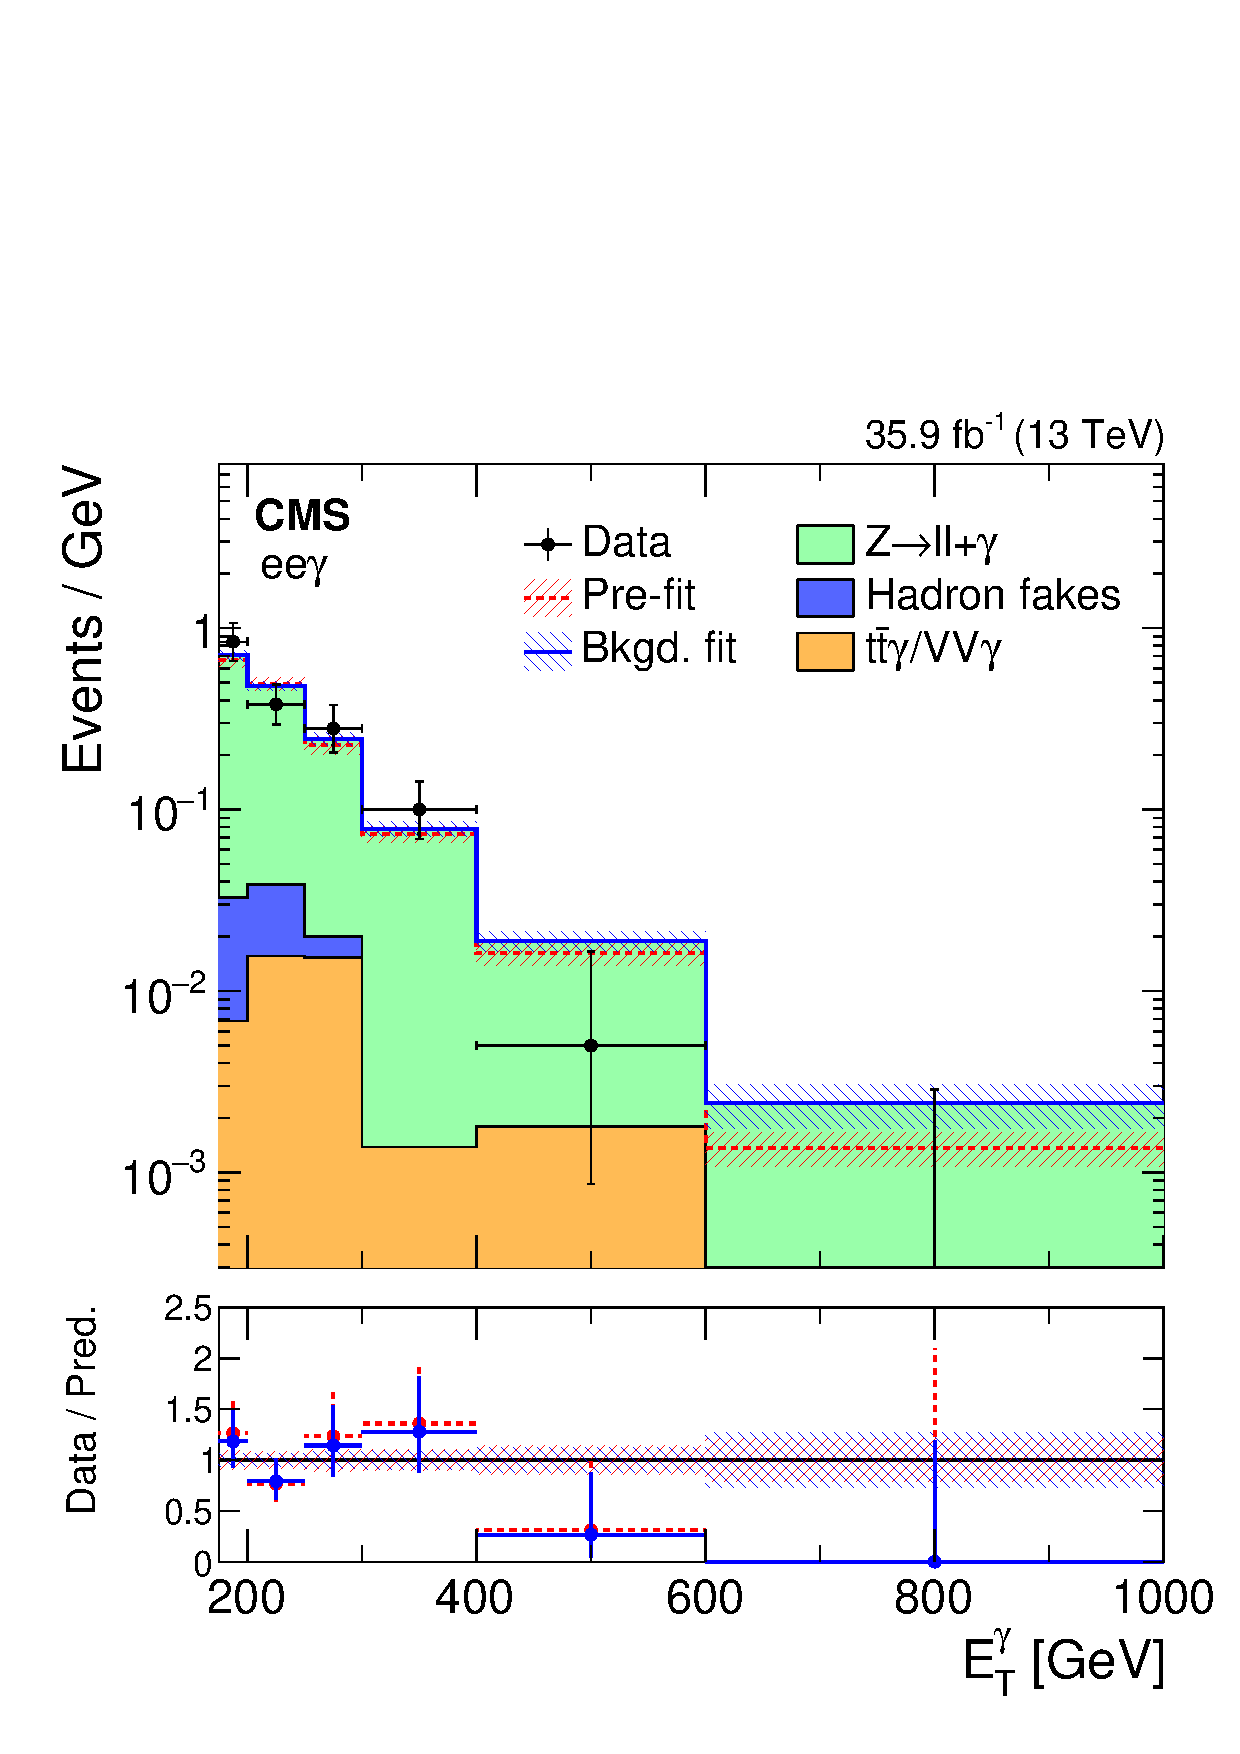
\includegraphics[width=0.49\textwidth]{Analysis/Figures/bonly_diel.pdf}
    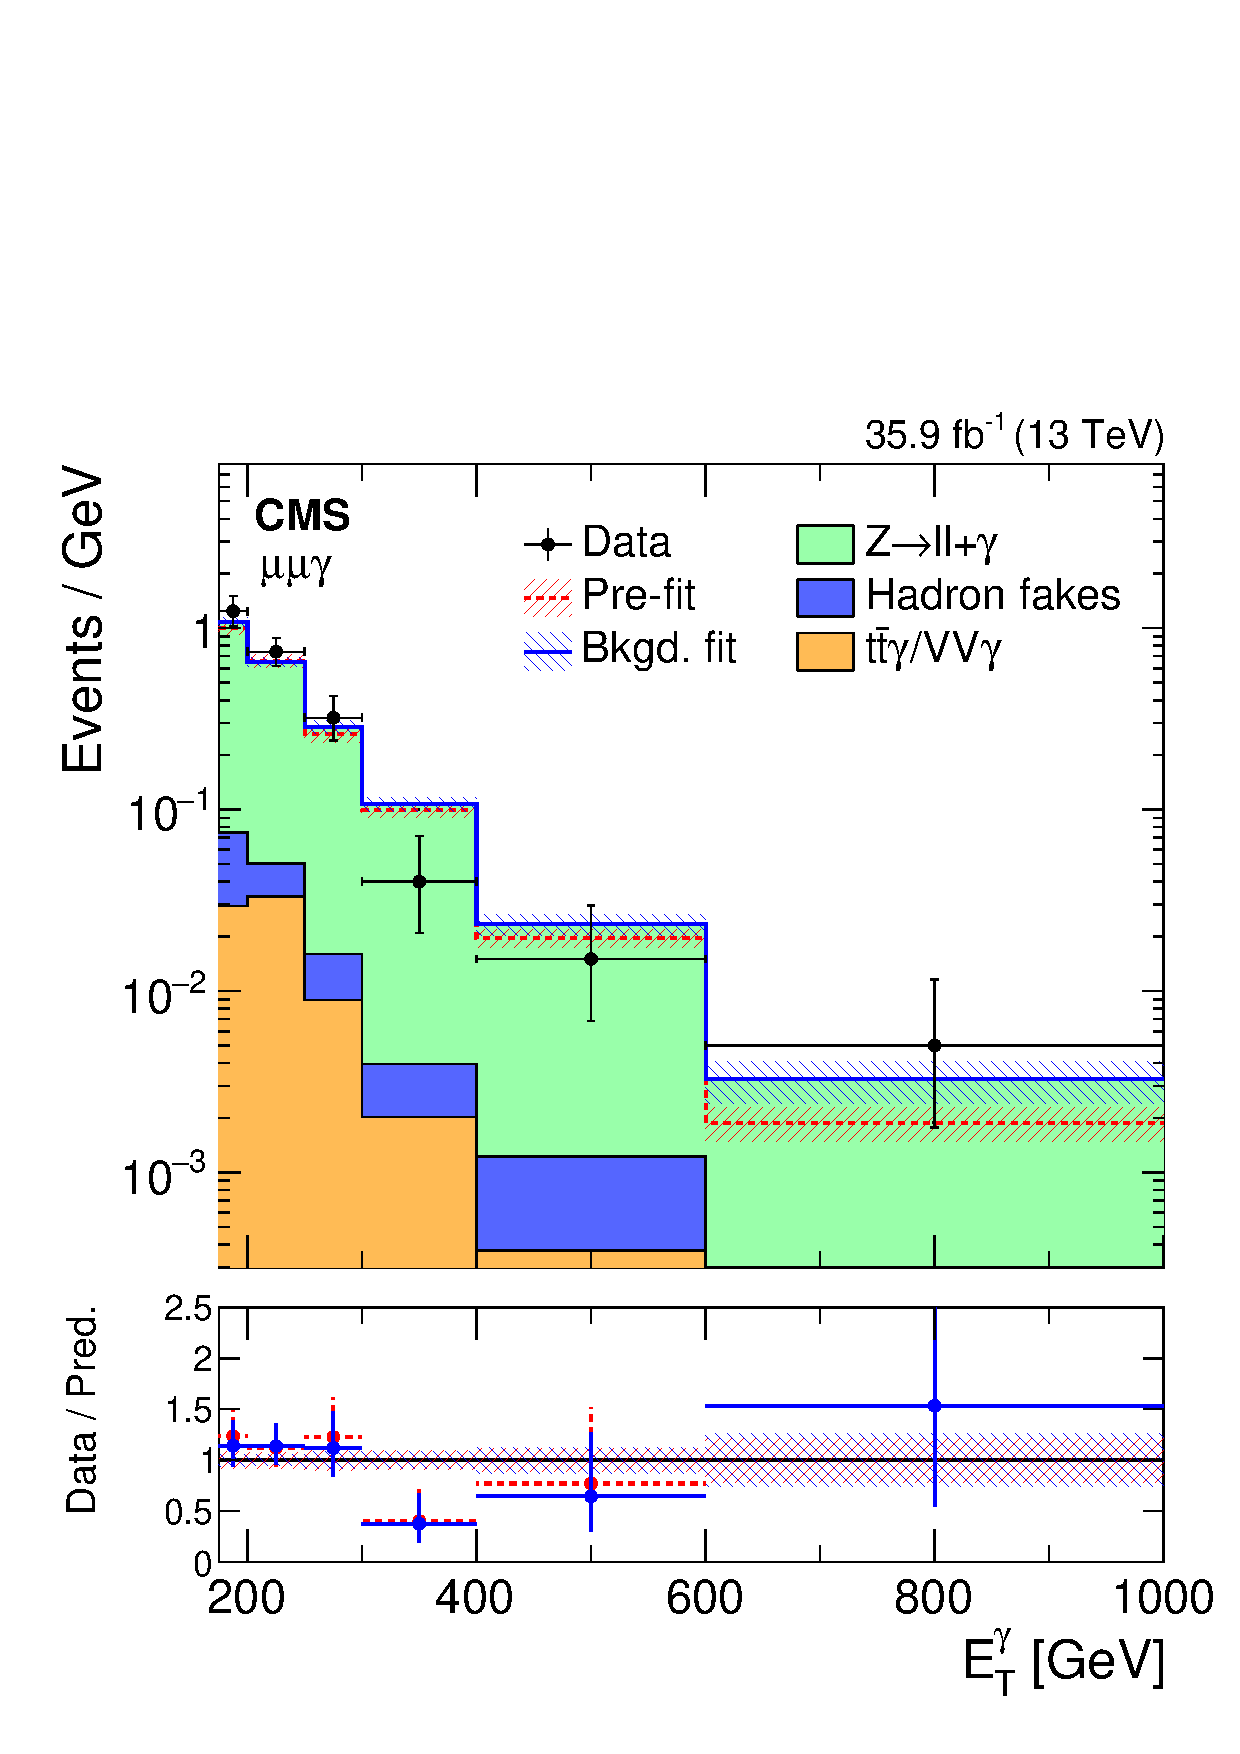
\includegraphics[width=0.49\textwidth]{Analysis/Figures/bonly_dimu.pdf}
    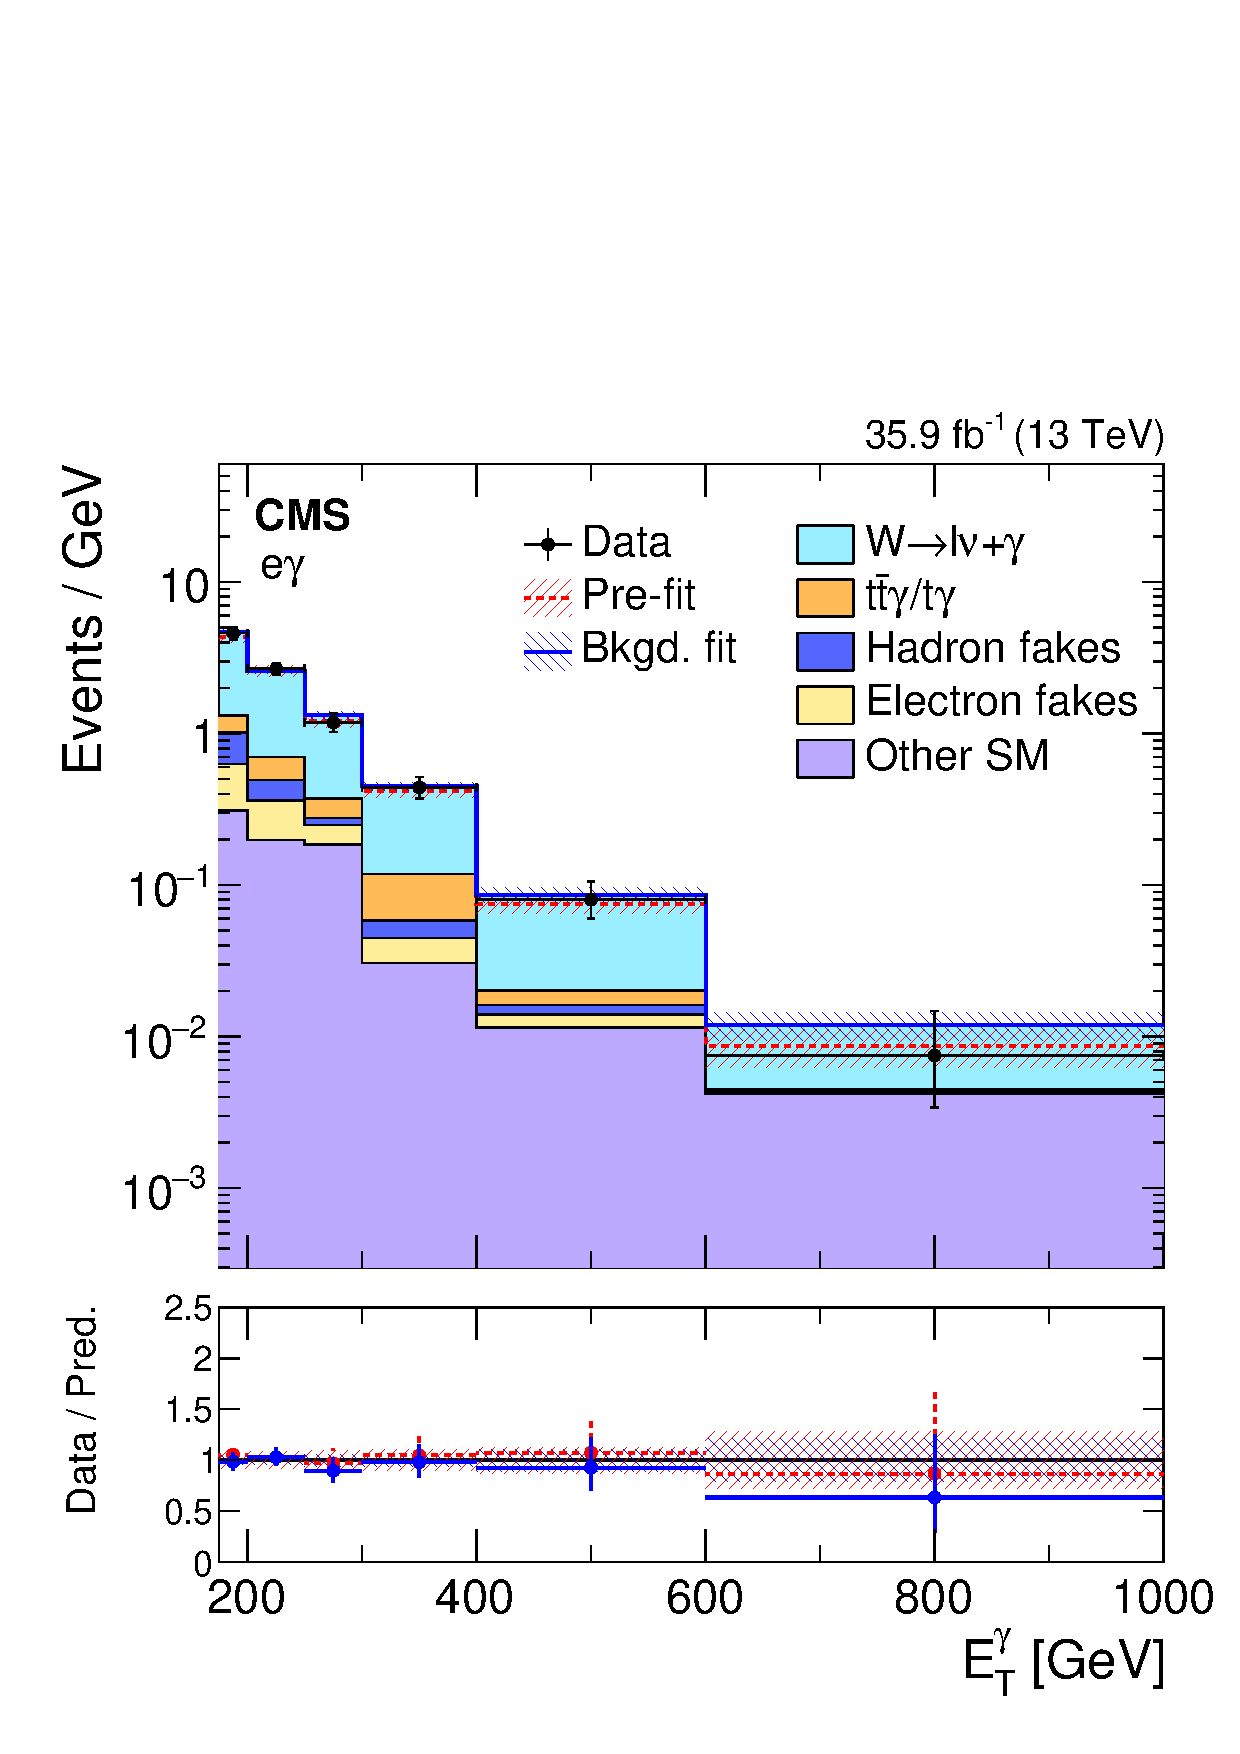
\includegraphics[width=0.49\textwidth]{Analysis/Figures/bonly_monoel.pdf}
    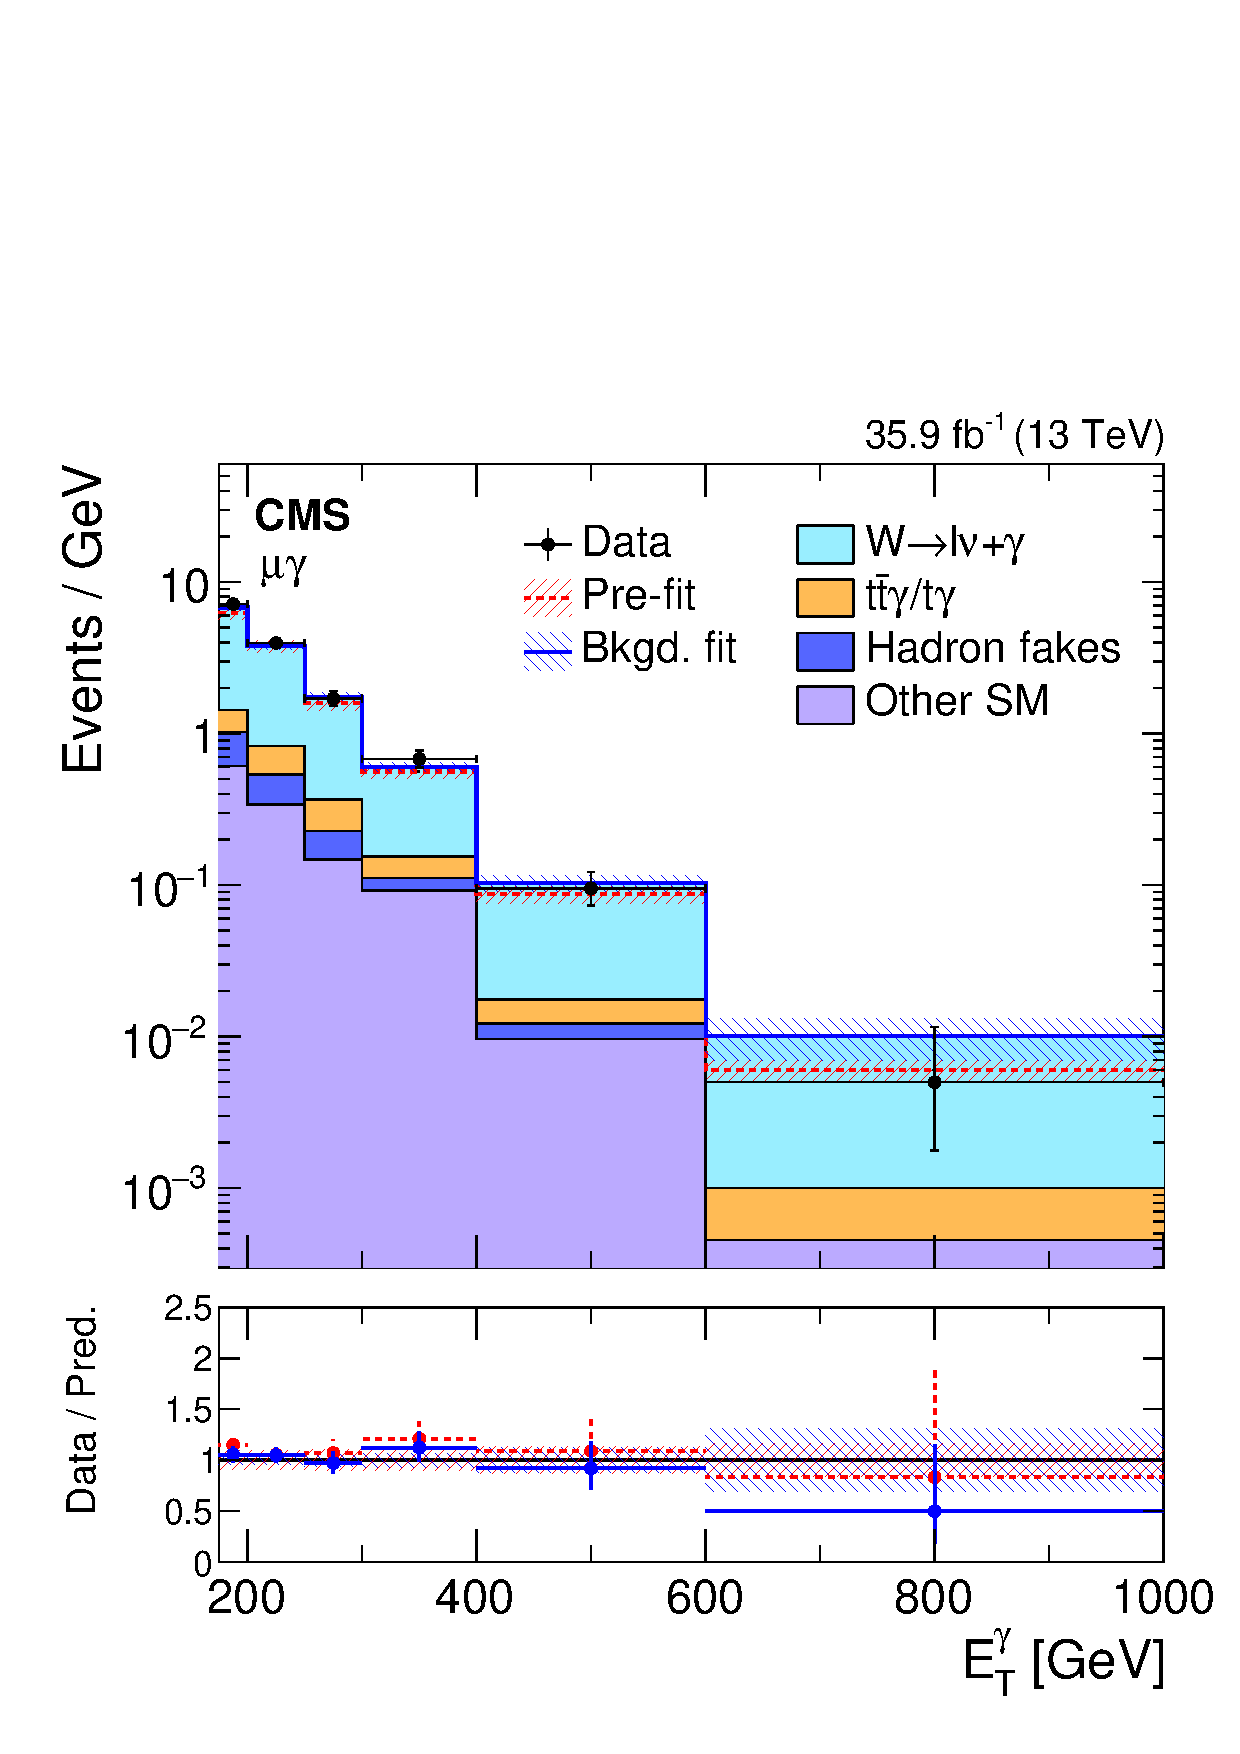
\includegraphics[width=0.49\textwidth]{Analysis/Figures/bonly_monomu.pdf}
    \caption{
      Comparison between data and MC simulation in the four control regions: 
      \Pe\Pe\Pgg\ (upper left), 
      \Pgm\Pgm\Pgg\ (upper right), 
      \Pe\Pgg\ (lower left), 
      \Pgm\Pgg\ (lower right) 
      before and after performing the simultaneous fit across all the control samples and signal region, and assuming absence of any signal.
      The last bin of the distribution includes all events with $\ETg > 1000\GeV$. 
      The ratios of data with the pre-fit background prediction (red dashed) and post-fit background prediction (blue solid) are shown in the lower panels. 
      The bands in the lower panels show the post-fit uncertainty after combining all the systematic uncertainties.
}
    \label{fig:postfitCR}
\end{figure}

\begin{figure}[htbp]
  \centering
    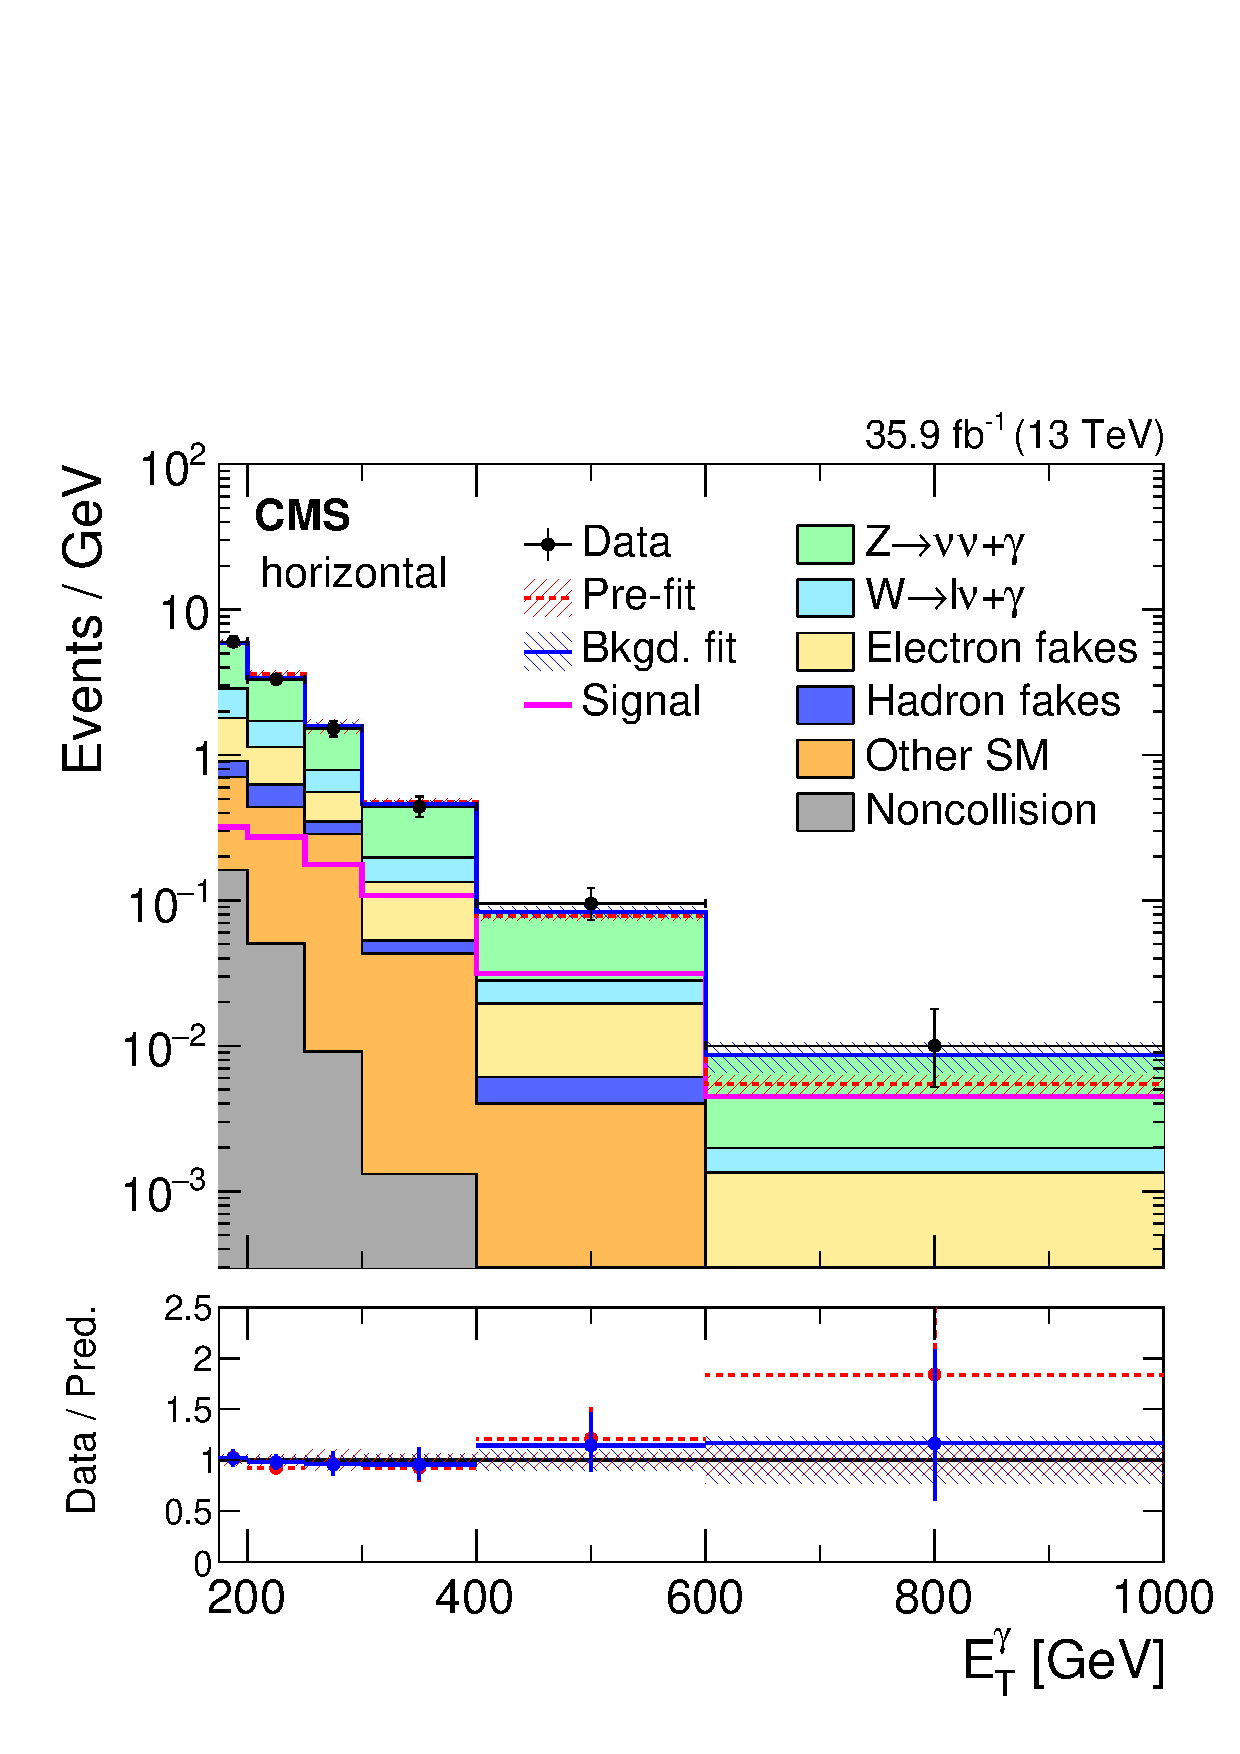
\includegraphics[width=0.49\textwidth]{Analysis/Figures/bonly_horizontal.pdf}
    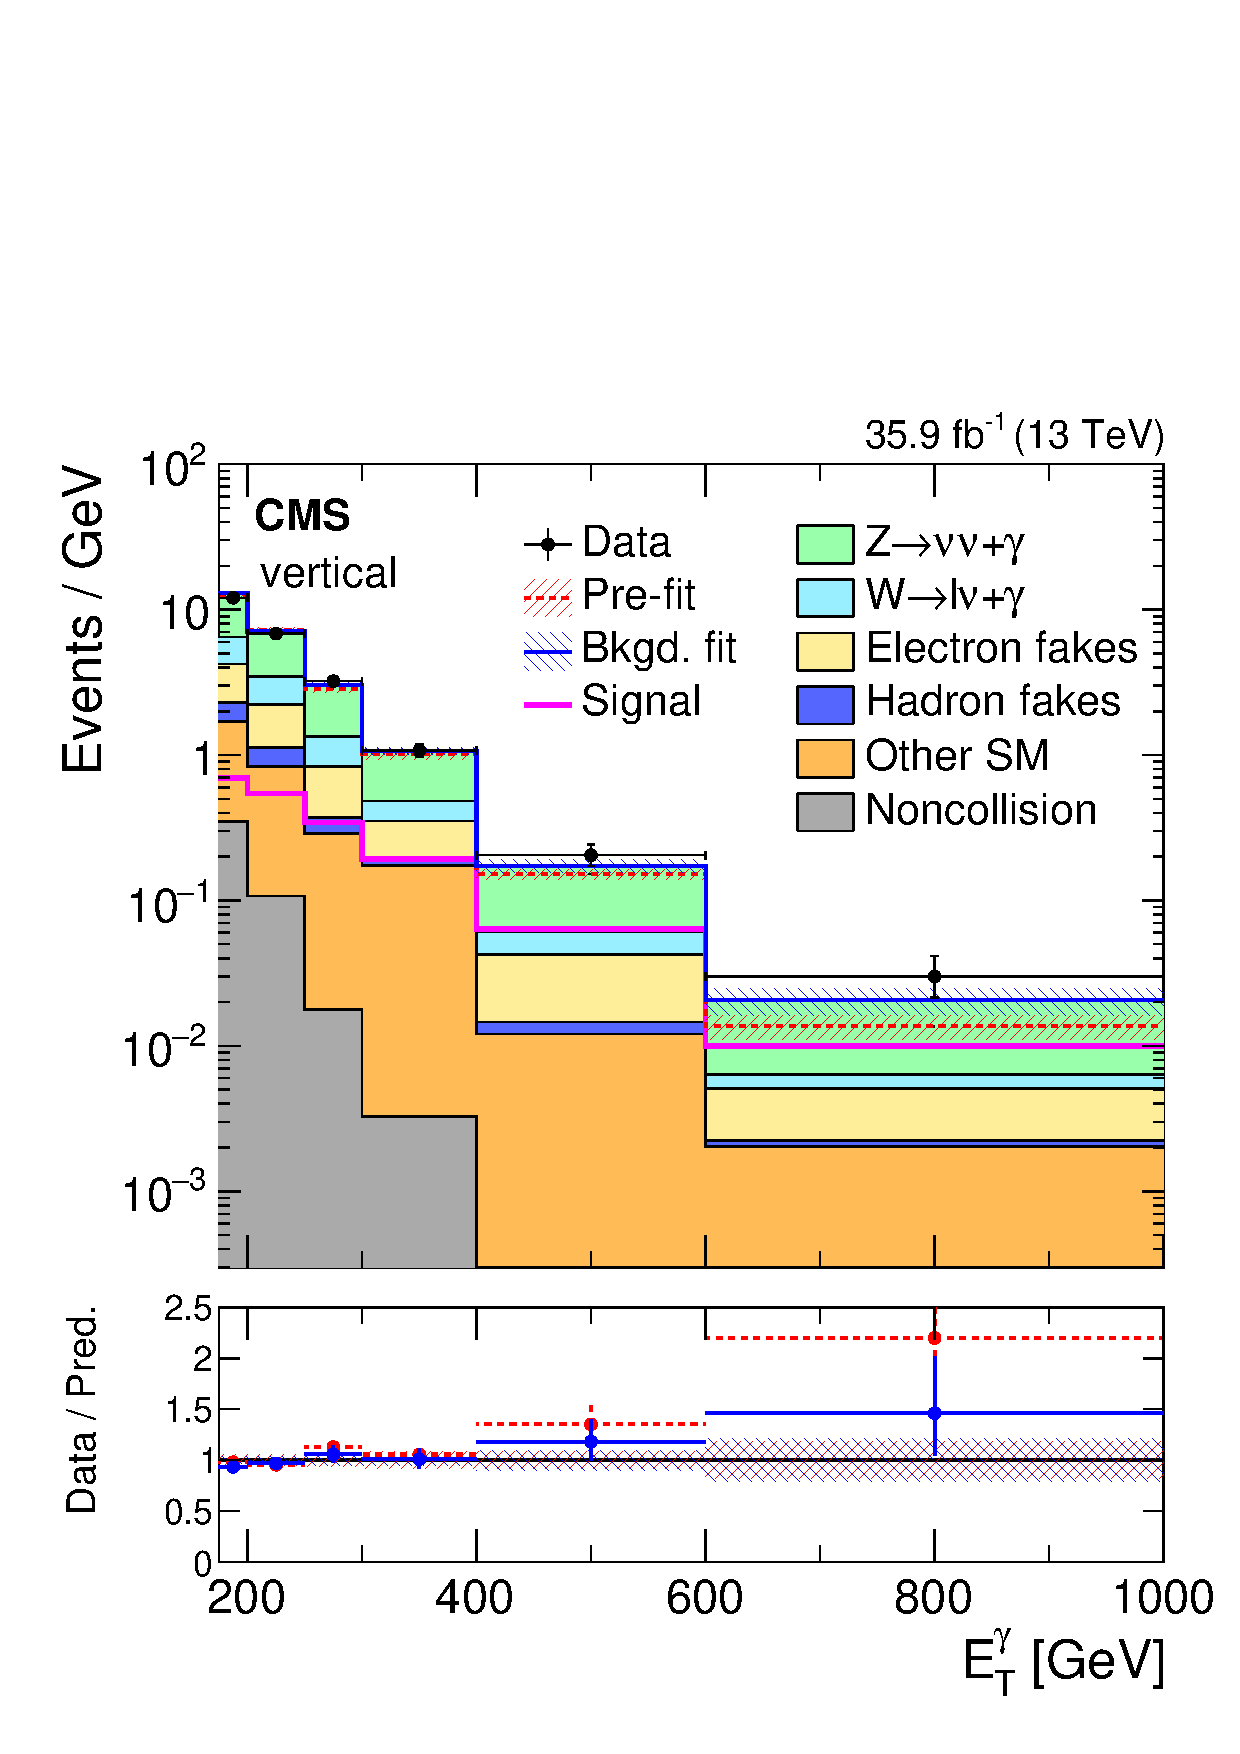
\includegraphics[width=0.49\textwidth]{Analysis/Figures/bonly_vertical.pdf}
    \caption{
      Observed \ETg\ distributions in the horizontal (left) and vertical (right) signal regions compared with the post-fit background expectations for various SM processes.
      The last bin of the distribution includes all events with $\ETg > 1000\GeV$. 
      The expected background distributions are evaluated after performing a combined fit to the data in all the control samples and the signal region. 
      The ratios of data with the pre-fit background prediction (red dashed) and post-fit background prediction (blue solid) are shown in the lower panels. 
      The bands in the lower panels show the post-fit uncertainty after combining all the systematic uncertainties. 
      The expected signal distribution from a 1\TeV vector mediator decaying to 1\GeV DM particles is overlaid.
    }
    \label{fig:postfitSR}
\end{figure}

Figure~\ref{fig:postfitCR} shows the observed \ETg\ distributionsin the four control regions compared with the results from simulations before and after performing the simultaneous fit across all the control samples and signal region, and assuming absence of any signal.
Figure~\ref{fig:postfitSR} shows the observed \ETg\ distributions in the horizontal and vertical signal regions compared with the results from simulations before and after performing a combined fit to the data in all the control samples and the signal region. 
The observed distributions are in agreement with the prediction from SM and noncollision backgrounds.

\begin{table}[htbp]
\centering
\begin{tabular}{ l|cccccc }
\rule[-1.2ex]{0pt}{3.8ex}\ETg~[\GeVns{}]      &         [175,  200] &         [200,  250] &         [250,  300] &         [300,  400] &         [400,  600] &         [600, 1000] \\
\hline
$\PZ\Pgg$        & $  81.2 \pm   8.0 $ & $  88.2 \pm   8.4 $ & $  38.8 \pm   4.8 $ & $  26.8 \pm   3.7 $ & $   8.8 \pm   1.9 $ & $   1.4 \pm   0.7 $ \\
$\PW\Pgg$        & $  27.9 \pm   3.7 $ & $  29.9 \pm   3.9 $ & $  11.4 \pm   1.7 $ & $   6.3 \pm   1.2 $ & $   1.4 \pm   0.4 $ & $   0.1 \pm   0.1 $ \\
Misid. electrons & $  22.5 \pm   2.7 $ & $  25.7 \pm   2.7 $ & $  10.5 \pm   1.0 $ & $   8.2 \pm   0.7 $ & $   2.7 \pm   0.2 $ & $   0.5 \pm   0.0 $ \\
Misid. hadrons   & $   5.2 \pm   2.2 $ & $   9.3 \pm   1.8 $ & $   3.1 \pm   0.7 $ & $   1.0 \pm   0.3 $ & $   0.4 \pm   0.1 $ & $   0.0 \pm   0.0 $ \\
Other SM         & $  13.6 \pm   2.0 $ & $  19.6 \pm   1.3 $ & $  13.9 \pm   0.4 $ & $   4.2 \pm   0.2 $ & $   0.8 \pm   0.0 $ & $   0.1 \pm   0.0 $ \\
ECAL spikes      & $   4.3 \pm   1.3 $ & $   2.7 \pm   0.8 $ & $   0.5 \pm   0.1 $ & $   0.1 \pm   0.0 $ & $   0.0 \pm   0.0 $ & $   0.0 \pm   0.0 $ \\
Total prediction & $ 154.6 \pm   8.3 $ & $ 175.4 \pm   8.8 $ & $  78.2 \pm   5.3 $ & $  46.6 \pm   4.0 $ & $  14.1 \pm   2.1 $ & $   2.1 \pm   0.8 $ \\
\hline
Observed         & $ 150   \pm  12   $ & $ 166   \pm    13 $ & $  76.0 \pm   8.7 $ & $  44.0 \pm   6.6 $ & $  19.0 \pm   4.4 $ & $   4.0 \pm   2.0 $ \\
\end{tabular}
\caption{Expected event yields in each \ETg\ bin for various background processes in the horizontal signal region.
         The background yields and the corresponding uncertainties are obtained after performing a combined fit to data in all the control samples, excluding data in the signal region.
         The observed event yields in the horizontal signal region are also reported.}
\label{tab:yield_mask_horizontal}

\end{table}

\begin{table}[htbp]
\centering
\begin{tabular}{ l|cccccc }
\rule[-1.2ex]{0pt}{3.8ex}\ETg~[\GeVns{}]      &         [175,  200] &         [200,  250] &         [250,  300] &         [300,  400] &         [400,  600] &         [600, 1000] \\
\hline
$\PZ\Pgg$        & $ 172   \pm    17 $ & $ 190   \pm  18   $ & $  83   \pm  10   $ & $  58.6 \pm   7.9 $ & $  18.0 \pm   3.9 $ & $   3.1 \pm   1.6 $ \\
$\PW\Pgg$        & $  59.9 \pm   7.8 $ & $  63.6 \pm   7.8 $ & $  24.6 \pm   3.5 $ & $  13.4 \pm   2.4 $ & $   3.0 \pm   0.8 $ & $   0.3 \pm   0.2 $ \\
Misid. electrons & $  48.4 \pm   5.6 $ & $  56.2 \pm   5.1 $ & $  23.4 \pm   1.8 $ & $  15.7 \pm   1.4 $ & $   5.6 \pm   0.4 $ & $   1.2 \pm   0.1 $ \\
Misid. hadrons   & $  15.1 \pm   4.4 $ & $  14.5 \pm   3.1 $ & $   4.2 \pm   0.8 $ & $   2.3 \pm   0.8 $ & $   0.5 \pm   0.1 $ & $   0.1 \pm   0.1 $ \\
Other SM         & $  33.8 \pm   4.1 $ & $  36.6 \pm   2.7 $ & $  13.6 \pm   0.5 $ & $  17.1 \pm   0.6 $ & $   2.4 \pm   0.1 $ & $   0.8 \pm   0.0 $ \\
ECAL spikes      & $   9.3 \pm   2.8 $ & $   5.7 \pm   1.7 $ & $   0.9 \pm   0.3 $ & $   0.3 \pm   0.1 $ & $   0.0 \pm   0.0 $ & $   0.0 \pm   0.0 $ \\
Total prediction & $ 339   \pm  18  $ & $ 366   \pm  19   $ & $ 150   \pm  11   $ & $ 107.5 \pm   8.7 $ & $  29.6 \pm   4.3 $ & $   5.4 \pm   1.7 $ \\
\hline
Observed         & $ 301   \pm  17   $ & $ 342   \pm  19   $ & $ 161 \pm  13   $ & $ 107   \pm  10   $ & $  41.0 \pm   6.4 $ & $  12.0 \pm   3.5 $ \\
\end{tabular}
\caption{Expected event yields in each \ETg\ bin for various background processes in the vertical signal region.
         The background yields and the corresponding uncertainties are obtained after performing a combined fit to data in all the control samples, excluding data in the signal regions.
         The observed event yields in the vertical signal region are also reported.}
\label{tab:yield_mask_vertical}
\end{table}

The expected yields in each bin of \ETg\ for all backgrounds in the horizontal and vertical signal regions after performing a combined fit to data in all the control samples, excluding data in the signal regions, are given in Tables~\ref{tab:yield_mask_horizontal} and~\ref{tab:yield_mask_vertical}, respectively.
The covariances between the predicted background yields across all the \ETg~bins in the two signal regions are shown in Fig.~\ref{fig:correlation_matrix}.
The expected yields together with the covariances can be used with the simplified likelihood
approach detailed in Ref.~\cite{CMS-NOTE-2017-001} to reinterpret the results for models not studied in this thesis

\begin{figure}[hbtp]
  \centering
  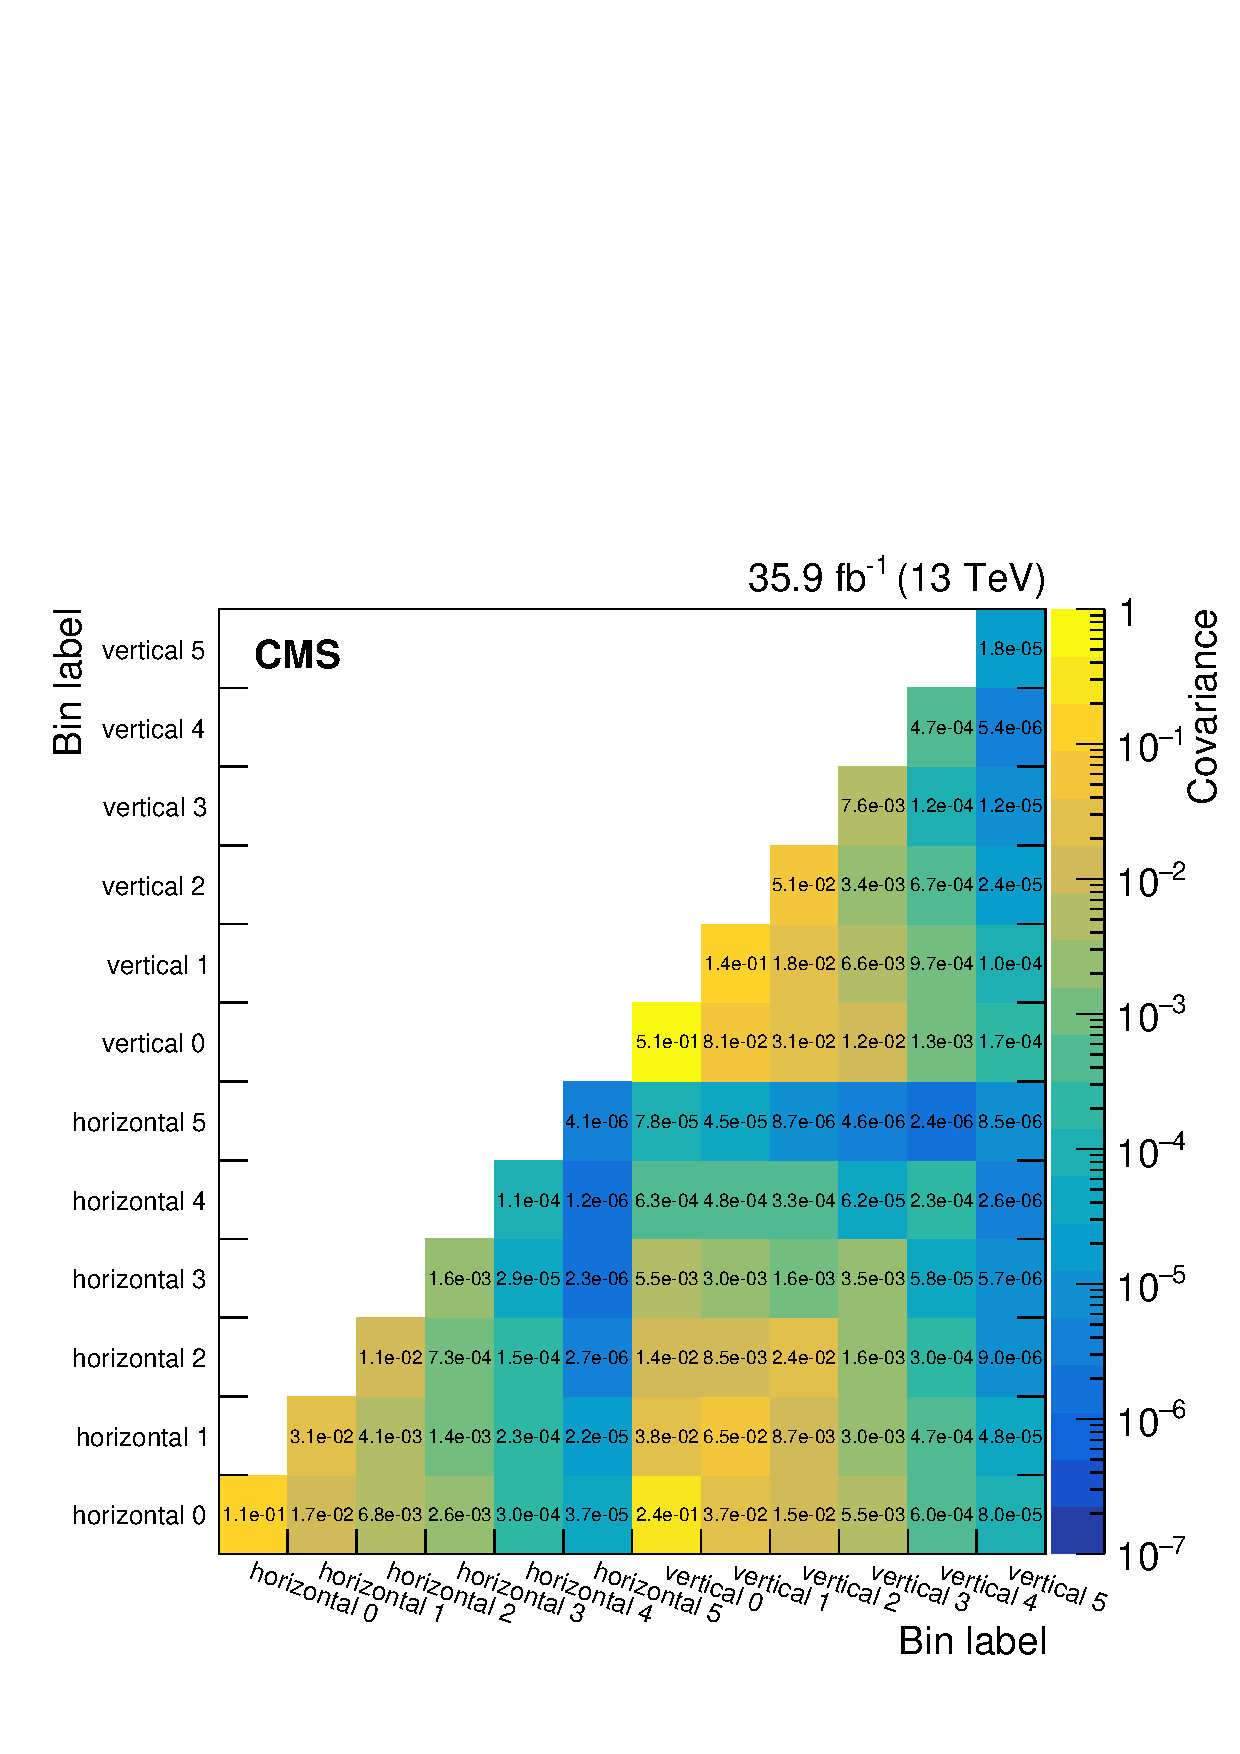
\includegraphics[width=0.9\textwidth]{Analysis/Figures/correlation_matrix.pdf}
  \caption{
    Covariances between the predicted background yields in all the \ETg\ bins of the horizontal and vertical signal regions.
    The bin labels specify which signal region the bin belongs to and what number bin it is for that region.}
  \label{fig:correlation_matrix}
\end{figure}.

\subsection{Limits}
\label{sec:limits}

No significant excess of events beyond the SM expectation is observed. 
Upper limits are determined for the production cross section of the new-physics processes mentioned in Section~\ref{sec:dmsimp}. 
For each model, a 95\% confidence level (\CL) upper limit is obtained utilizing the asymptotic \CLs\ criterion~\cite{Junk:1999kv,Read:2002hq,Cowan:2010js}, using a test statistic based on the negative logarithm of the likelihood in Section~\ref{sec:interpretation}.

\begin{figure}[htbp]
  \centering
    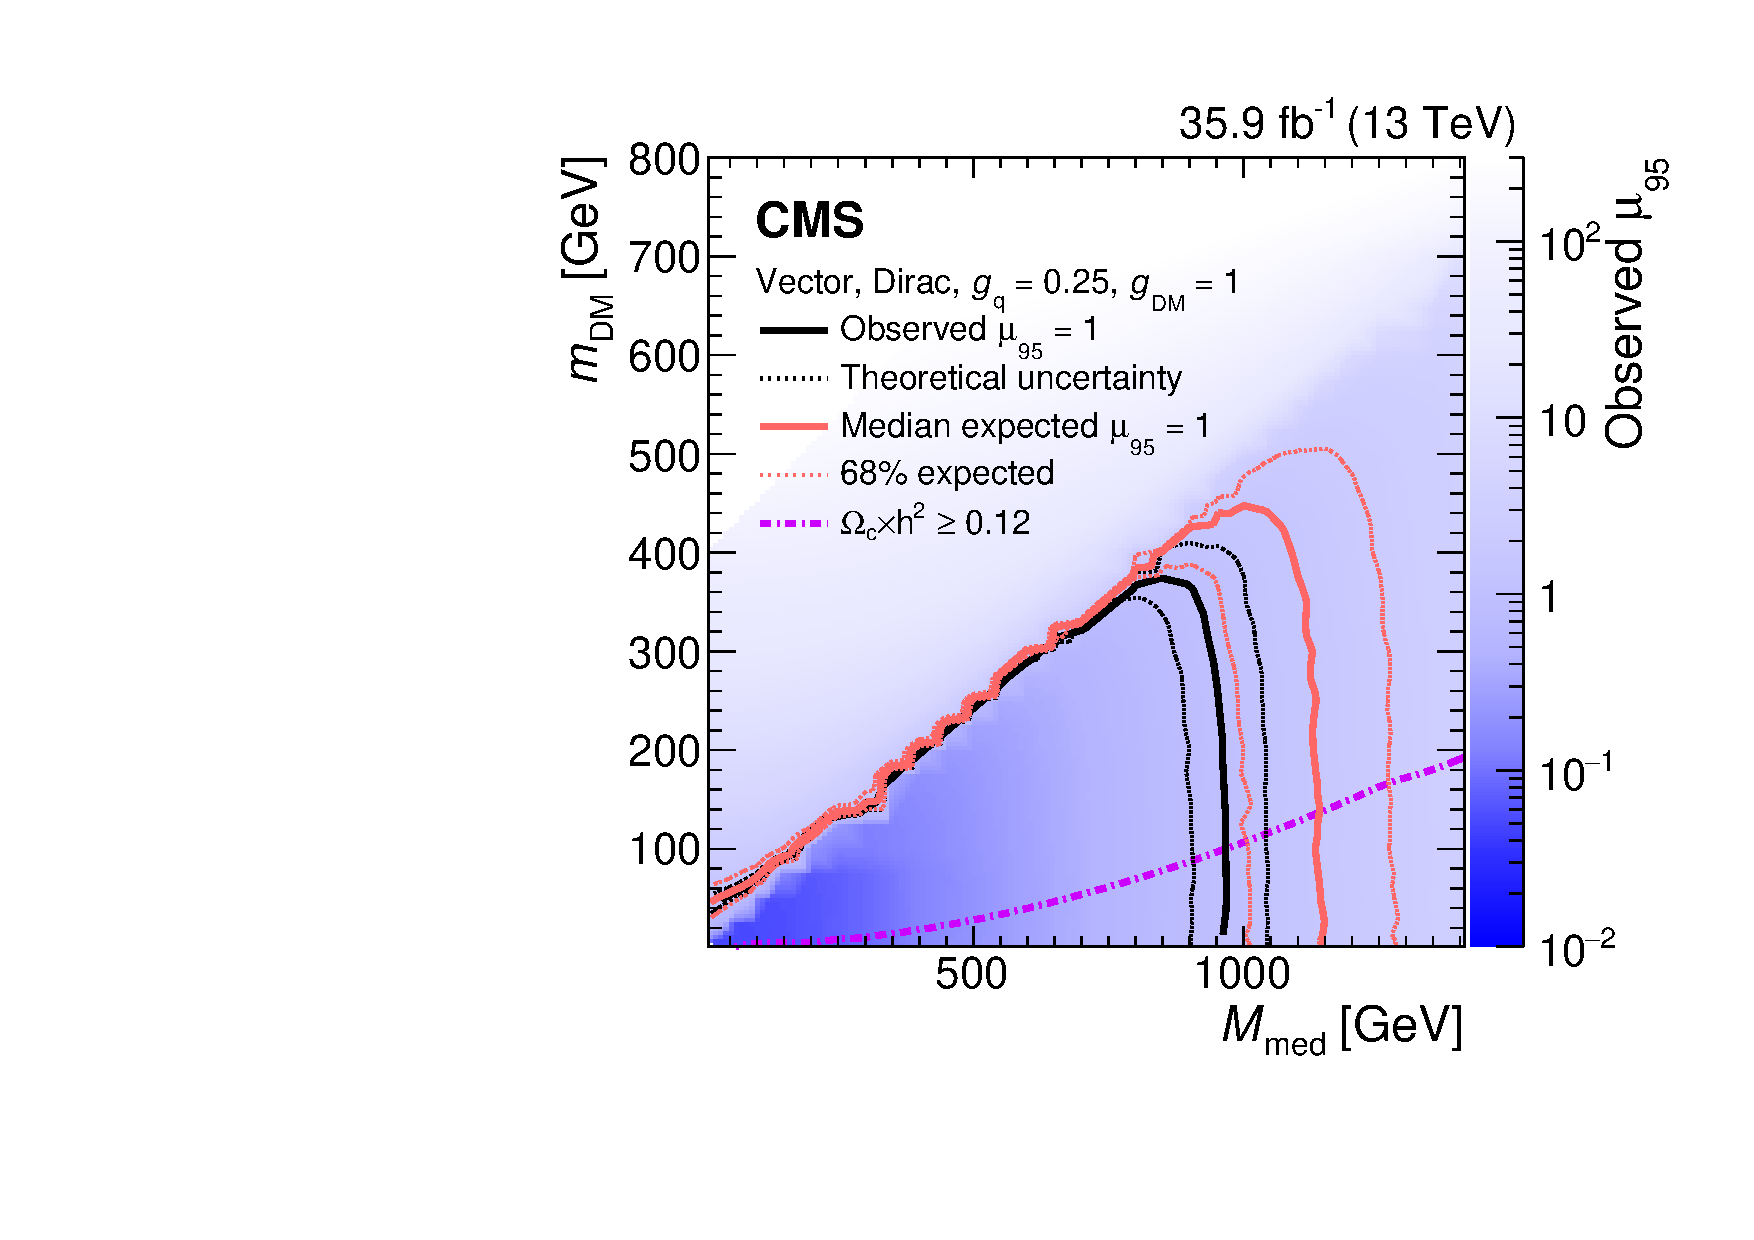
\includegraphics[width=0.45\textheight]{Analysis/Figures/limits_vector.pdf}
    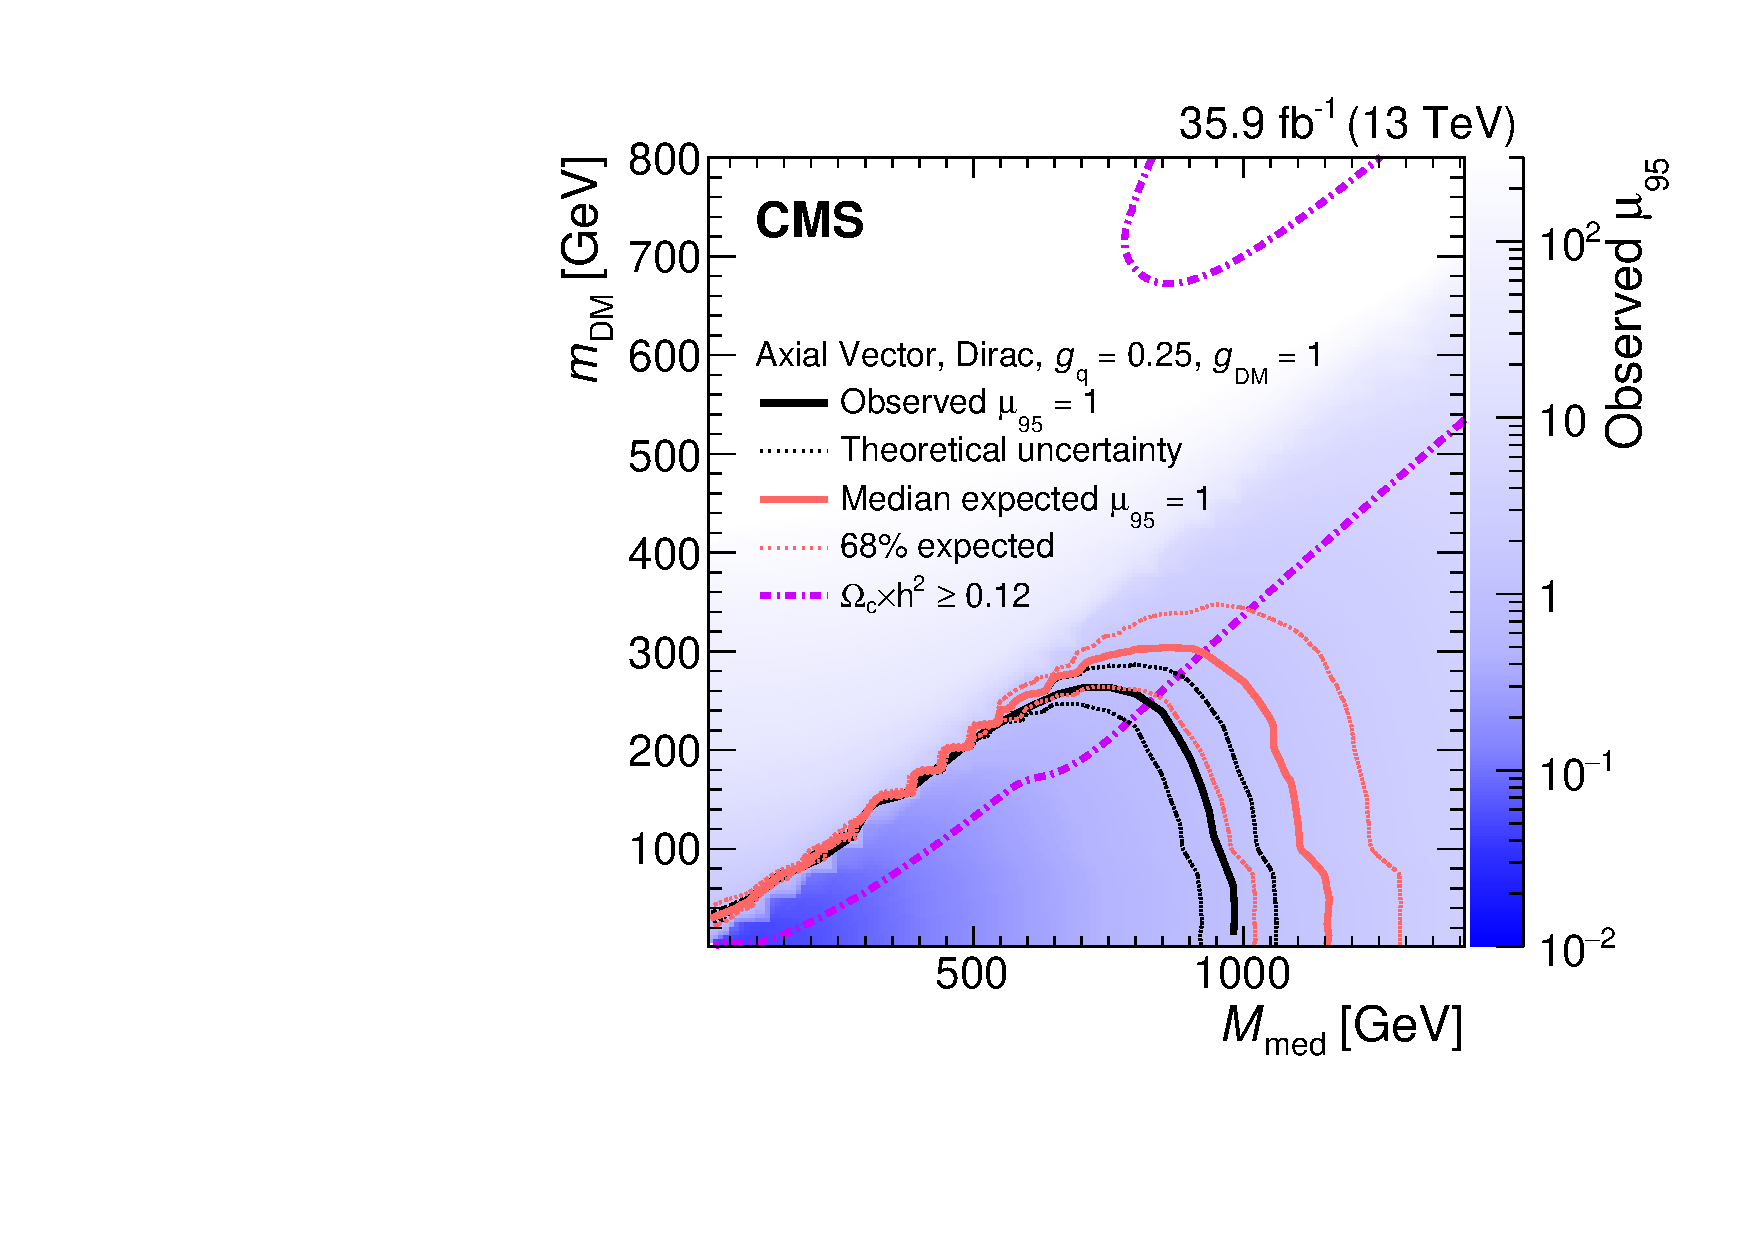
\includegraphics[width=0.45\textheight]{Analysis/Figures/limits_axial.pdf}
    \caption{
      The ratio of 95\% \CL\ upper cross section limits to the theoretical cross section ($\mu_{95}$), for DM simplified models with vector (top) and axial-vector (bottom) mediators, assuming $\gq=0.25$ and $\gdm=1$.
      Expected $\mu_{95} = 1$ contours are overlaid in red. 
      The region under the observed contour is excluded. For DM simplified model parameters in the region below the lower violet dot--dash contour, and also above the corresponding upper contour in the right hand plot, cosmological DM abundance exceeds the density observed by the Planck satellite experiment.
    }
    \label{fig:limits}
\end{figure}

Figure~\ref{fig:limits} shows the 95\% \CL\ upper cross section limits with respect to the corresponding theoretical cross section ($\mu_{95}= \sigma_{95\%}/\sigma_{\text{theory}}$) for the  vector and axial-vector mediator scenarios, in the \mmed--\mdm\ plane. 
The solid black (dashed red) curves are the observed (expected) contours of $\mu_{95} = 1$. 
The $\sigma_{\text{theory}}$ hypothesis is excluded at 95\% \CL\ or above in the region with $\mu_{95} < 1$. 
The uncertainty in the expected upper limit includes the experimental uncertainties. 
For the simplified DM LO models considered, mediator masses up to 950\GeV are excluded for values of \mdm\ less than 1\GeV.

The results for vector and axial-vector mediators are compared to constraints
from the observed cosmological relic density of DM as determined from measurements of the cosmic microwave background by the Planck satellite experiment~\cite{Ade:2015xua}.
The expected DM abundance is estimated, separately for each model, using the thermal freeze-out mechanism implemented in the {\sc MadDM}~\cite{Backovic:2013dpa} framework and  compared to the observed cold DM density $\Omega_c h^2=0.12$~\cite{Ade:2015xua}, where $\Omega_c$ is the DM relic abundance and $h$ is the dimensionless Hubble constant.

\begin{figure}[htbp]
  \centering
    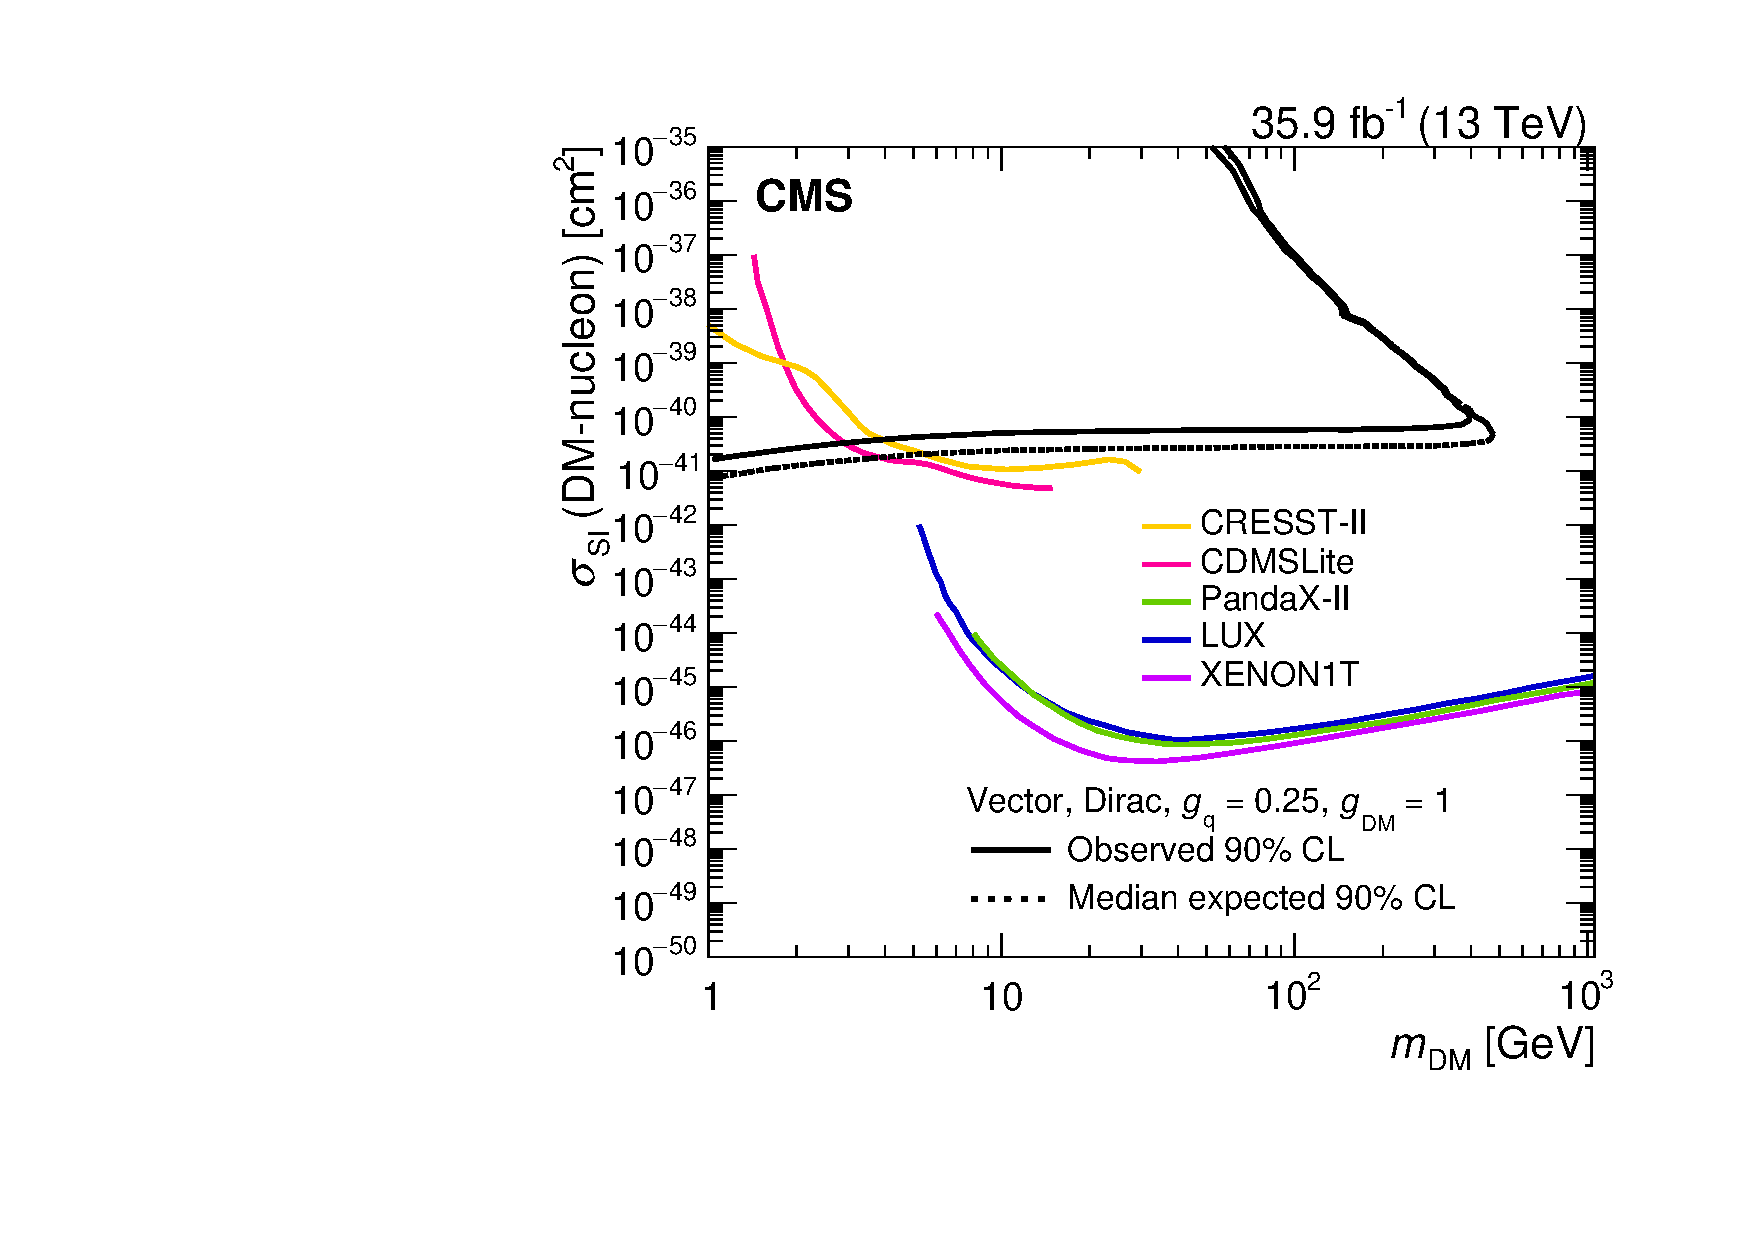
\includegraphics[width=0.45\textheight]{Impact/Figures/limits_direct.pdf}
    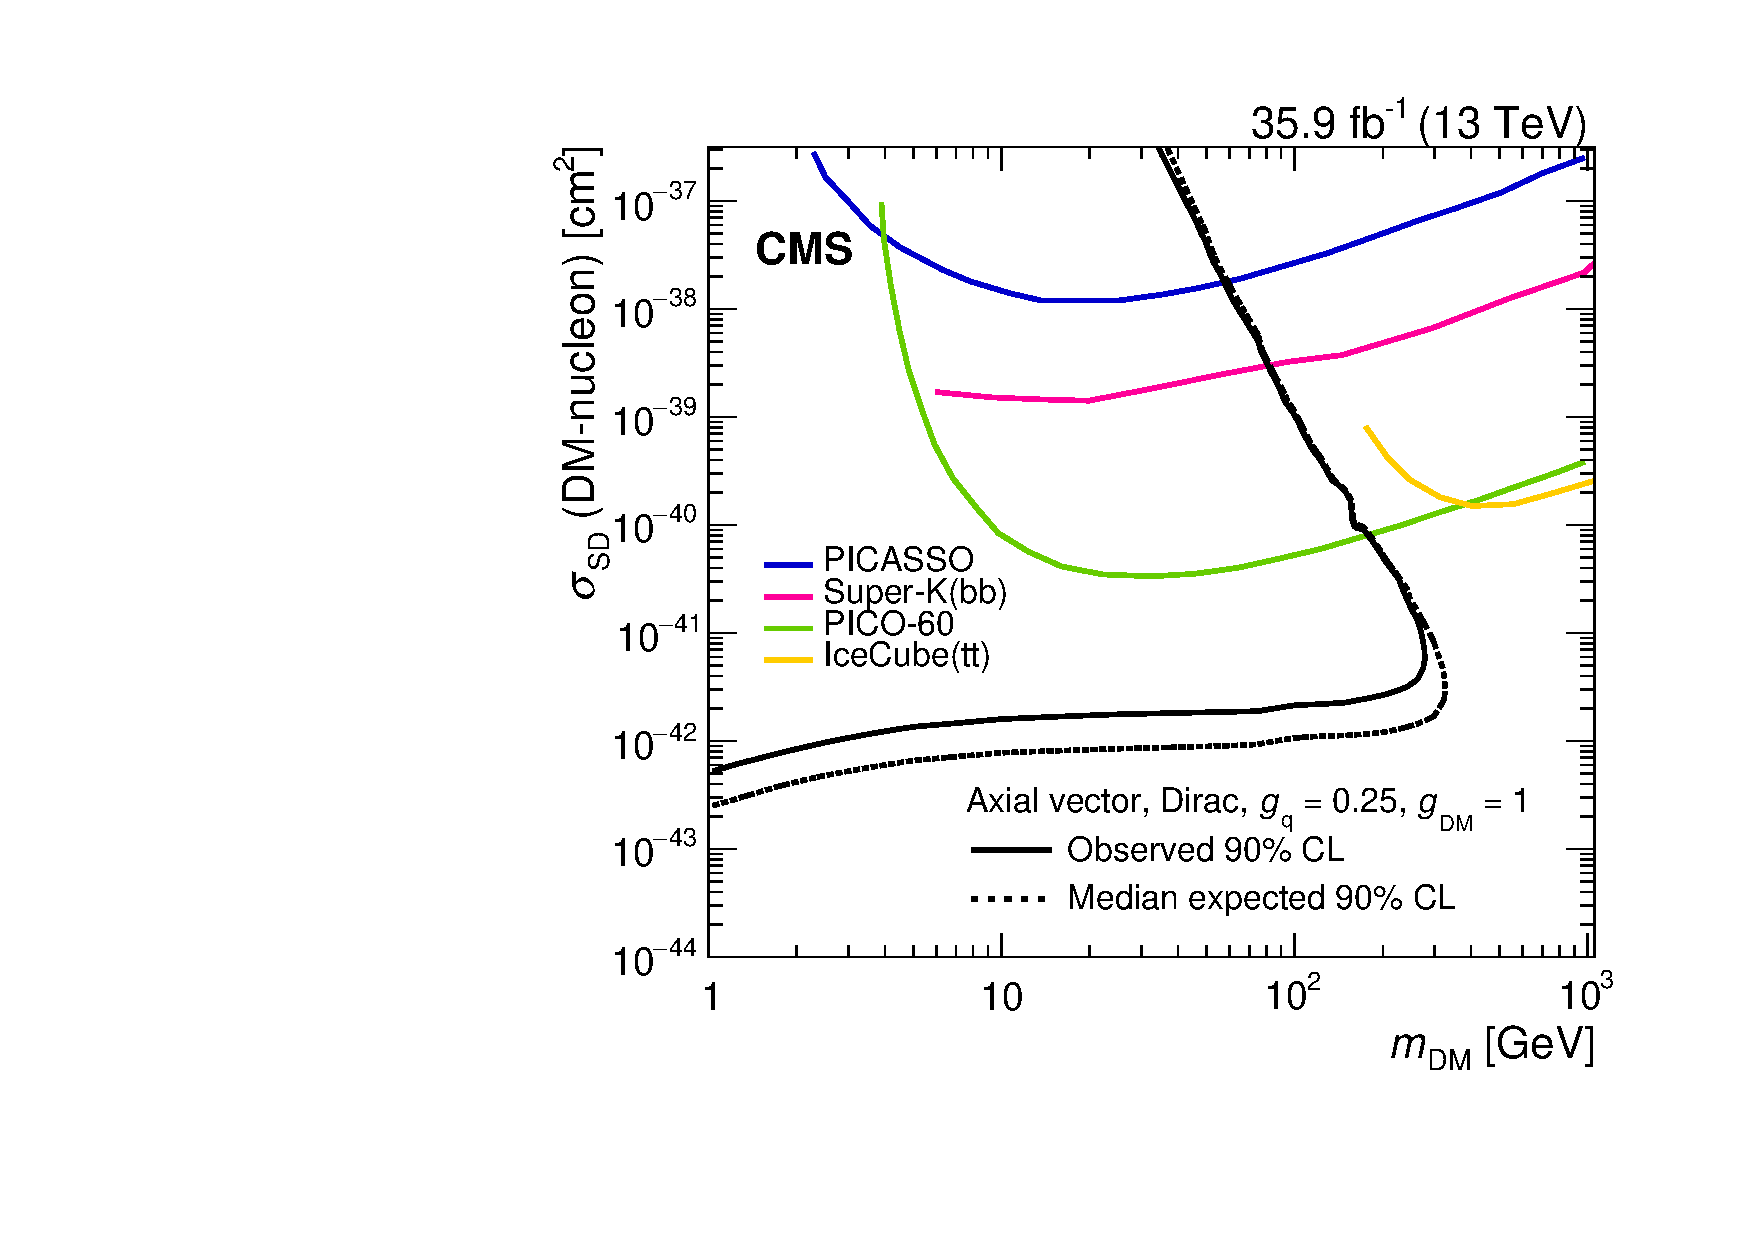
\includegraphics[width=0.45\textheight]{Impact/Figures/limits_indirect.pdf}
    \caption{
      The 90\% \CL\ exclusion limits on the $\chi$--nucleon spin-independent scattering cross sections involving the vector operator (top) and the $\chi$--nucleon spin-dependent scattering cross sections involving the axial-vector operator (bottom) as a function of the \mdm.
      Simplified model DM parameters of $\gq=0.25$ and $\gdm=1$ are assumed.
      The region to the upper left of the contour is excluded. 
      On the plots, the median expected 90\% \CL\ curve overlaps the observed 90\% \CL\ curve.
      Also shown are corresponding exclusion contours, where regions above the curves are excluded, from the recent results by the direct and indirect detection experiments listed in the text.
    }
    \label{fig:limits_direct}
\end{figure}

To enable a direct comparison with results from direct and indirect detection experiments, the 95\% \CL limits on the mediator mass for the vector and axial-vector models are translated to 90\% \CL limits on the spin-independent and spin-dependent DM--nucleon scattering cross sections, $\sigma_{\text{SI}}$ and $\sigma_{\text{SD}}$ respectively, following the prescriptions given in Ref.~\cite{Boveia:2016mrp} and~\cite{dmforum}.
The exclusion contours for the vector and axial-vector models shown in Figure~\ref{fig:limits} are translated into the $\sigma_{\text{SI}}$--\mdm\ and $\sigma_{\text{SD}}$--\mdm\ planes shown in Figure~\ref{fig:limits_direct}. 
When compared to recent results by the CDMSLite~\cite{Agnese:2015nto}, LUX~\cite{Akerib:2016vxi}, PandaX-II~\cite{Cui:2017}, XENON1T~\cite{Aprile:2018}, and CRESST-II~\cite{Angloher:2015ewa} collaborations, the limits obtained from this search provide stronger constraints for DM masses less than 2\GeV for spin independent models.
When compared to recent results by the PICO-60~\cite{Amole:2017dex}, IceCube~\cite{Aartsen:2016exj}, PICASSO~\cite{Behnke:2016lsk} and Super-Kamiokande~\cite{Choi:2015ara} collaborations, the limits obtained from this search provide stronger constraints for DM masses less than 200\GeV for spin dependent models.
